%http://texblog.org/2012/08/29/changing-the-font-size-in-latex/
\documentclass[12pt]{report}
\usepackage{amsfonts, amsmath, amsthm, amssymb}
\usepackage[urlcolor=blue,linkcolor=black,colorlinks=true]{hyperref}
\hypersetup{
  pdftitle = {A Novel Approach to Detecting Covert DNS Tunnels Using Throughput
Estimation},
  pdfkeywords = {},
  pdfauthor = {Michael Himbeault}
}
%\usepackage[headsep=1cm,headheight=50pt]{geometry}
\usepackage[dvips]{graphicx}
\usepackage{subfigure}
\usepackage{lscape}

\usepackage[toc,page]{appendix}

% http://tex.stackexchange.com/questions/5091/what-to-do-to-switch-to-biblatex
% http://polyphys-s01.ethz.ch/images/bibstyles/
%\usepackage[natbib=true,style=numeric-verb,backend=bibtex]{biblatex}
%\addbibresource{../Reference/bibliography.bib} % Syntax for version >= 1.2
\bibliographystyle{amsplain}

\usepackage{setspace}

\addtolength{\oddsidemargin}{-.5in}
\addtolength{\evensidemargin}{-.5in}
\addtolength{\textwidth}{1in}

\addtolength{\topmargin}{-.5in}
\addtolength{\textheight}{1in}

\newcommand{\hreff}[2]{\href{#1}{#2}\footnote{\url{#1}}}

\newtheorem{thm}{Theorem}[section]
\newtheorem{cor}[thm]{Corollary}
\newtheorem{lem}[thm]{Lemma}

\newtheorem*{hyp}{Hypothesis}

\theoremstyle{remark}
\newtheorem{remark}[thm]{Remark}

\theoremstyle{definition}
\newtheorem{definition}[thm]{Definition}

\theoremstyle{definition}
\newtheorem{example}{Example}[section]

\theoremstyle{definition}
\newtheorem{algorithm}{Algorithm}[section]

\begin{document}
%\title{A Novel Approach to Detecting Covert DNS Tunnels Using Throughput
%Estimation}
%\author{Michael Himbeault}

%\title{
%\huge{\textbf{An In-memory Database for Prototyping Anomaly Detection Algorithms at Gigabit Speeds}}\\[1.75cm]
%\Large{by} \\ [0.5cm]
%\Large{Travis Friesen} \\ [1.2cm]
%\Large{A Thesis\\
%Submitted to the Faculty of Graduate Studies\\
%of the University of Manitoba\\
%in partial fulfilment of the requirements\\
%for the degree of}\\[1cm]    
%\Large{MASTER OF SCIENCE}\\[1cm]
%\Large{Department of Electrical and Computer Engineering\\
%University of Manitoba\\
%Winnipeg} \\
%%\Large{Advisors: Bob McLeod, Ph.D., P.Eng.\\
%%Paul Card, Ph.D.}\\
%\vfill
%\Large{Copyright \copyright 2013 by Travis Friesen}
%}
%% \author{} \date{}
%% \date{Decembruary 2012.5}
%\date{}
%
%\maketitle

\pagestyle{empty}

\begin{titlepage}
\centerline{\huge{A Novel Approach to Detecting Covert DNS}}
\vspace{10mm}
\centerline{\huge{Tunnels Using Throughput Estimation}}
\vspace{20mm}
\centerline{by}
\vspace{5mm}
\centerline{\large{Michael Himbeault}}
\vspace{20mm}
\centerline{\large{A Thesis}}
\vspace{3mm}
\centerline{\large{Submitted to the Faculty of Graduate Studies}}
\vspace{3mm}
\centerline{\large{of the University of Manitoba}}
\vspace{3mm}
\centerline{\large{in partial fulfilment of the requirements}}
\vspace{3mm}
\centerline{\large{for the degree of}}
\vspace{13mm}
\centerline{\LARGE{MASTER OF SCIENCE}}
\vspace{15mm}
\centerline{\large{Department of Electrical and Computer Engineering}}
\centerline{\large{University of Manitoba}}
\centerline{\large{Winnipeg, Manitoba, Canada}}
\vspace{30mm}
\centerline{\large{Copyright \copyright 2013 Michael Himbeault}}
\centerline{}
\vfill
\centerline{\today}
\end{titlepage}

\doublespacing
% http://www.sce.carleton.ca/faculty/chinneck/thesis.html

% ==============================================================================
% The abstract should make sense to everyone.
% It should give them an idea of whether they possess the background necessary
% to understand the paper, and if they do, what the paper will tell them.
% ==============================================================================

\abstract{In a world that relies very heavily on data, protection of that data and protection
of the \emph{motion} of that data is of the utmost importance. Covert
communication channels attempt to circumvent established methods of control,
such
as firewalls and proxies, by utilizing non-standard means of getting messages
between two endpoints. The Domain Name System (DNS), the system that translates
text-based resource names into machine-readable resource records, is a very
common and effective platform upon which covert channels can be built. This work
proposes, and demonstrates the effectiveness of, a novel technique thatf
estimates data transmission throughput over DNS in order to identify the
existence of a DNS tunnel against the background noise of legitimate network
traffic. The proposed technique is robust in the face of the obfuscation
techniques that are able to hide tunnels from existing detection methods.}


\addtocontents{toc}{\protect\thispagestyle{empty}}
\addtocontents{lot}{\protect\thispagestyle{empty}}
\addtocontents{lof}{\protect\thispagestyle{empty}}

\tableofcontents
\listoftables
\listoffigures

\newpage


% ==============================================================================
% The introduction should make sense to people with the necessary background,
% and should be of moderate use to people without the necessary background. It
% should introduce the problem we are trying to solve, why it is worth solving,
% give a coarse picture of where our solution sits in the landscape of
% solutions, and what the solution involves. It should briefly touch on the
% outcome of the solution.
% ==============================================================================

\pagestyle{plain}
\setcounter{page}{1}

\chapter{Introduction}

Control of the data that moves between hosts on a computer network is vitally
important in order to be able to enforce security policies and protect sensitive
information. To this end systems such as firewalls, proxies, and content filters
are put into place in order to monitor and control network traffic. Covert
channels are utilized to circumvent these control mechanisms for purposes that
range from benign to malicious. This work focuses specifically on DNS tunnels,
however other types of covert channels do exist.

Detecting a DNS tunnel effectively on a busy network link becomes an exercise in
discrimination. Since there is such a wide variety of network traffic that is
generated on a busy link, there is generally no simple definition of
\emph{normal} for a particular class of traffic, including DNS. This tends to
either rule out, or decrease the viability of, algorithms that depend on finding
a definition of normal and alerting based on deviations from that norm.

A highly sensitive and specific detection of DNS tunnels on a busy network link
is an important problem in the arena of network security as it enables
administrators to block or otherwise control these potential sources of
compromise. A non-exhaustive, but informative, list of potential uses for covert
channels (including DNS tunnels) is:

\begin{itemize} \item Data exfiltration \item Communication through restrictive
firewalls \item Receiving commands or information from a remote source \item
Transport layer for complete VPN solutions \end{itemize}

In enterprises that deal with sensitive data such as financial, health,
personal or intellectual property information, it is of the utmost importance to
control the access to this information. Even if an enterprise does not have
information that needs protecting, DNS tunnels should still be blocked in order
to prevent malware from communicating\cite{Dietrich2011}. Because DNS tunnels can be used for
arbitrary communication, they can be used as command-and-control channels for
botnets\cite{WoframlAlpha-Botnet} or any other malicious system that relies on data transmission.
Preventing botnets from operating is in the best interest for the Internet as a
whole and should be a concern of every user of the Internet.

Existing algorithms for detection of DNS tunnels rely on one of two primary
methods, character frequency analysis and signatures, to detect the presence of
a DNS tunnel. The signature-based solutions attempt to identify portions of the
tunnelling application data (as opposed to the user data that is sent using the
tunnelling application) for which a signature can be built. These signature
based solutions are subject to many of the same problems that plague signature
based anti-virus solutions including their inability to detect zero-day
situations. For example, if the application changes its communication schemes,
the signatures may no longer be valid and may no longer trigger when they are
intended and expected to. Additionally, signatures cannot be built for
applications that are not available for study, or that are not known of. For
applications that use a custom communication scheme that has not had a signature
built specifically for it, it is very unlikely that an existing signature will
be relevant and will successfully detect it.

Because signature based schemes are not effective in detecting DNS tunnels in a
zero-day\footnote{\emph{Zero-day} refers to a situation where nothing is known
about the attack as it has never been seen or analyzed before.} situation,
another method is required. Analysis based on character frequency is proposed
in\cite{Born2010.cfa} by Kenton Born with similar approaches proposed by several
other authors (see section \ref{litreview-dns} for more details) which uses
character frequency analysis under some assumed properties. More details are
given in section \ref{litreview-dns-cfa}.

Due to the weaknesses listed above, it is clear that a new approach is necessary
that detects DNS tunnels in a zero-day situation and without the known weakness
involving character frequency and probabilistic encoding. A demonstration of
this weakness is given in section \ref{appendix-probcode}. This work proposes,
and demonstrates the effectiveness of, a method of detecting DNS tunnels that
meets these requirements.

The proposed method operates under the assumption that DNS tunnels move more
data than a normal domain but don't necessarily do it by moving more bytes than
a benign domain. This distinction is important since, on a busy network, a large
content or service provider such as Google, Amazon, Facebook or Twitter may make
up orders of magnitude more DNS traffic by byte count than a DNS tunnel. By
leveraging this fact, it is possible to detect any use of DNS to transmit
arbitrary data by measuring the amount of data that is transmitted using a
particular DNS domain or subdomain. The details of this measurement methodology
are contained in chapter \ref{proposed-method} and requires estimating the
amount of unique data that is transmitted by analyzing the queries themselves
and not simply counting characters in the query string.

This proposed detection methodology is shown to detect DNS tunnels in as few as
ten packets (as shown in section \ref{test-existing} and continues to be robust
in highly hostile detection environments such as those that contain a great deal
of non-tunnel traffic as well as benign uses of DNS for transmitting arbitrary
data\footnote{Many security vendors utilize the fact that DNS and UDP port 53
are so loosely controlled in order to ensure that their deployed devices can
communicate with the vendor intelligence unimpeded.}. Detector performance on
commodity hardware is shown to scale to greater than two gigabits of UDP port 53
throughput per second, indicating that this methodology does not sacrifice
performance for detection accuracy and remains practical for monitoring very
large networks.

\newpage

% ==============================================================================
% The background section provides a reasonable breadth and depth of content for
% people to brush up enough to understand the literature review, problem at hand
% and solution. It should provide references for breadth and depth not covered
% in this section.
% ==============================================================================
\chapter{Background}

\section{Entropy}
Entropy\cite{WolframAlpha-EntropyWord}\cite{WolframAlpha-EntropyMath} is
intuitively speaking, a measure of how random a particular collection of items
is. In the context of a random variable, entropy is a measure of the uncertainty
in the output of the random variable. A random variable that has a distribution
that outputs a particular symbol seventy five percent of the time has
considerably less uncertainty, and thus less entropy, than one that outputs all
symbols with equal frequency. In the context of a collection of symbols in a
stream, or data source, entropy can be though of as a measure of the information
content of that collection. If the collection comprises almost entirely a single
symbol, then that collection can be thought of as containing less information,
and thus having less entropy, than a collection where all symbols occur with
equal frequency.

Entropy can be calculated for a collection of symbols
$\mathcal{C}=\{c_1,\ldots,c_n\}$ with symbol $c_i$ appearing with proportion
$0\leq p_i\leq 1$ where $\sum_{i=1}^n{p_i}=1$ as

 \[H(\mathcal{C})=-\sum_{i=1}^n{p_i \log{p_i}}\]

The base of the logarithm determines the units of the resulting value. If a
logarithm in base 2 is used, then the entropy has the units of \emph{bits}, if
the logarithm with the natural base $e$ is used then the entropy has the units
of \emph{nats}, and if the logarithm is in the common base 10, then the entropy has
the units of \emph{digits}.

\section{Domain Name System (DNS)}

DNS is the service through which names are mapped to
resources\cite{rfc1034}\cite{rfc1035}. Typically, this maps a name (such as
\emph{www.google.ca}) to an IP address. The value of this service is that names
are considerably more flexible, and typically considerably easier to remember,
than the resource or record that they point to. For example, \emph{google.com}
is considerably easier to remember than one of the IP addresses that it points
to, such as 74.125.226.34. \emph{google.com} is also considerably more flexible,
since it points to not just one but several addresses, and successive responses
will receive different records in a round-robin, or random, fashion. This
rotation of responses allows for a crude, but natural, form of load balancing
and automatic fail over, while retaining its ease of use.

The DNS protocol is assigned both User Datagram Protocol (UDP) and Transmission
Control Protocol (TCP) port 53 for communication with most communication
operating over UDP as opposed to TCP. The use of TCP depends on the
implementation of the resolver, however the specification indicates the TCP
should be used if the response data exceeds 512 bytes or during a zone
transfer\cite{rfc1035}. Domain Name System Security Extensions (DNSSEC), due to
the fact that it requires a signature of authenticity for all responses, will
often cause the response to require TCP\cite{rfc4034}. Because there are no
restrictions on when TCP may be used, some resolvers may be implemented to use
TCP for all responses as this does not violate the specifications for DNS.

%http://www.iana.org/assignments/dns-sec-alg-numbers/dns-sec-alg-numbers.xml

The experiments related to this work do not consider the situation of DNS over
TCP since the analysis techniques are identical due to the fact that the formats of the UDP and
TCP responses is identical once the TCP stream is reassembled. Modification of
the tools developed for this work would require the ability to perform TCP
stream reassembly in order to extract the responses from the TCP response\footnote{A tool that performs this reassembly is included in the same source distribution as the code for this work.}.

Because DNS is such an integral component of Internet communication it is not
generally reasonable to simply block it while still expecting functional
Internet connectivity. A common approach, called DNS \emph{proxying}, which
forces all DNS queries to be made to a DNS proxy server that is controlled by
the interested entity (Internet Service Provider (ISP), company, etc...). This DNS proxy server is
responsible for handling all DNS queries for the internal network, and any DNS
queries that are destined for the Internet (as opposed to the proxy) are
typically dropped by the firewall in this type of configuration. The DNS proxy
server operates in \emph{recursive mode}, which means that if a question is
asked of it to which it does not know the answer, the proxy server will then
query for the answer (by issuing its own query to the global DNS system) and
then respond to the initial request using the response from the global network.

DNS is a heavily cached protocol due to how often data can be reused between
queries. Consider how often a desktop Internet user causes a request for
\emph{google.com}. If a request had to traverse the entire DNS system every
time, this would represent a very considerable amount of traffic being
generated. To avoid this, every DNS record has extra information about it that
includes, among other things, how long it can be cached for. Standard caching
lengths put it around one hour which means that a DNS server will only
recursively pass on a query for a record once an hour. This caching period is
not constant and can be set differently, depending on the information the record
contains. Some records require a considerably lower Time To Live (TTL), as low
as one minute, while for others a considerably longer duration (months) may be
appropriate.

This proxy architecture removes some naive operation modes for DNS tunnels that
will be discussed in in more detail in \ref{tunnels-types-raw}, but does not
offer any protection against the more sophisticated forms of DNS tunnels.

\section{Covert Channels}

Covert channels are methods of communication that use non-standard means of
communication for the purpose of evading detection and/or blocking by the
existing security infrastructure. Covert channels may utilize portions of an
existing protocol\cite{Born2010.psudp} or communication channel, or they may find ways of
transporting information utilizing a completely new medium. An example of the
latter is called a \emph{timing channel}\cite{Sellke2009}, which can utilize the timing between
packets to convey information. A timing channel carefully controls the timing
between packets sent to a remote server to encode information, thereby utilizing
a method of communication that is not utilized by any standardized protocol
or communication method.

Covert channels come in may forms and not all types support the properties that
are normally associated with a communication channel. Because they are built on
unorthodox, or unreliable, transmission media and are subject to the effects of
intermediate routing and networking devices they cannot always offer all of the
same functionality as a legitimate channel. For example, covert channels need
not support bi-directionality due to either the constraints of the underlying
medium, or the effect of intermediate devices. A covert channel that is only
useful for reception is one that utilizes a third-party image hosting service.
It is possible to embed arbitrary information into the header portion of an
otherwise completely benign JPEG image file\cite{isoeic10918-1} which could then
be posted to Facebook, Flickr, or any other publicly accessible image hosting
service. This image file can then be checked by the remote hosts to pull the
information however, due to the nature of the image services, the remote hosts
may have no way of posting information back to the other endpoint, thus making
the communication channel unidirectional.

Real time data transfer refers to the ability for a communication channel to
send data immediately. UDP, by its very nature, supports this and TCP supports
this via the PUSH flag which indicates that data is being sent before a full
window has been accumulated. The TCP PUSH flag is used, for example, during a
Secure Shell (SSH) connection in order to provide interactivity when typing and
viewing output. Timing channels, or any channel that relies on modifying normal
system traffic instead of generating their own traffic, by their nature, are
unable to support real time data transfer. This is because they need to wait for
a system packet in order to send their data, and if the system goes for a period
of time without sending data then the covert channel must wait as well.

\section{DNS Tunnels}
\label{tunnels-types}
DNS tunnelling is the method by which arbitrary data is transferred
over the same channels as DNS. DNS tunnels come in one of two primary types: raw, or
conforming.

\subsubsection{Raw DNS Tunnels}
\label{tunnels-types-raw}
Raw DNS tunnels do not attempt to mimic or conform to the DNS specifications,
and simply attempt to utilize the fact that UDP port 53 is often left relatively
uncontrolled in firewalls. Raw tunnels attempt to exploit this by transmitting
arbitrary traffic using UDP port 53 packets with arbitrary payload 
\footnote{Iodine demonstrates this behaviour when operating in its raw
transport mode}. This is the most efficient exploitation of the ubiquity of DNS
as it incurs the lowest amount of overhead, both computationally and in terms of
network throughput. The trade off for this efficiency is that it is the least
conforming and the most likely to get stopped by either a firewall or a proxy.
In the situation where all DNS queries are forced to be proxied through a
dedicated DNS server, raw DNS tunnels will fail to operate as expected. This is
because when the UDP port 53 traffic is redirected to the proxy, the DNS server
will attempt to interpret the arbitrary payload as a DNS packet and will likely
fail. When it fails, it will drop the packet thereby preventing all raw UDP port
53 communication. Because these types of tunnels are effectively blocked by
standard firewall and proxy practises, detection of these tunnels is not
considered in this work.

\subsubsection{Conforming DNS Tunnels}
\label{tunnels-types-conforming}
Conforming DNS tunnels produce DNS packets that conform to all appropriate
specification and RFC documents and, as far as any DNS server is concerned, the
traffic generated is valid DNS traffic. These tunnels incur the highest
computational and throughput overhead, but have the advantage that detecting and
blocking them is a very difficult process. The detection of this type of DNS
tunnels is the topic of this work. This type of tunnel is capable of operating
in almost any environment, even those with very strict firewall and proxy policies. Because
this type of tunnel operates in very hostile (to the operation of the tunnel)
environments, detection of this type of DNS tunnel is of interest to all levels
of government and industry.

Conforming DNS tunnels operate by embedding the data for transmission into the
query string and response, requiring a modified, non-conforming, server on one
end of the connection and a piece of software on the client end. Typically these
types of DNS tunnels have one endpoint that is controlled by the tunnel user,
with that controlled endpoint running dedicated server software. The client and
server software are responsible for transforming arbitrary information to and
from DNS queries and responses. The precise details of how the translation is
done between DNS and the raw data depends entirely on the implementation.

\subsubsection{DNS Tunnel Software}
\label{tunnels-existing}
Some existing DNS tunneling software currently available is OzymanDNS\cite{ozymandnssrc},
Iodine\cite{iodinesrc}, Dns2tcp\cite{dns2tcpsrc}, DNScat\cite{dnscatsrc} and
DeNiSe\cite{denisesrc}, and PSUDP\cite{psudpsrc}. Each of these have slightly
different operational characteristics, but they all aim to do the same thing,
which is transmission of arbitrary data over DNS.

Iodine supports raw tunnels, as well as moving information back from the server
in IPv4 addresses (A), mail server (MX), arbitrary text (TXT) and many other
supported DNS record types. TXT records are rarely used by consumers or end-user
applications, and so a blanket block policy of TXT records for end-user devices
would have very little impact on end-user applications. TXT records are as close
to a raw tunnel that a conforming tunnel can get to in terms of throughput since
they allow large blocks of largely uncontrolled content.

DNScat utilizes a type of DNS record that is an alias to another record (a CNAME
record) and a supplementary A record, when appropriate\footnote{The A record is
not actually used for throughput but rather to give a 'termination' point for a
sequence of CNAME records}. OzymanDNS and DeNiSe utilize solely the TXT record,
which is as close to the raw tunnel as possible, however can be easily blocked
by simply blocking TXT records. Because these tools only use TXT records it is
possible that they are the least flexible and deployable out of those listed
above given a hostile environment. Dns2tcp utilizes either TXT or KEY
records\footnote{Historically KEY records were used to transmit encryption
related keys, however their use has been phased out by other DNS record types}
which makes it as flexible as OzymanDNS and DeNiSe. The KEY DNS record was
designated for specific uses\cite{rfc2931}, but has been deprecated
now\cite{rfc3445} in favour of the DNSKEY record for use with
DNSSEC\cite{rfc3755} and IPSECKEY for use with IPSEC\cite{rfc4025}. Because of
this deprecation, use of the KEY record is subject to strict filtering which
greatly reduces the effectiveness of this solution.

All of the above tools utilize encoding and decoding mechanisms that would
successfully propagate through a proxy server, at the cost of the fact that the
tunnel applications have to generate their own traffic. PSUDP, proposed by
Kenton Born, aims to remove the latter requirement by creating slack space
within existing DNS packets at the UDP transport layer. He proposes two ways
of creating this slack space: naively placing it at the end of the packet, and
rearranging the DNS query string to utilize pointers to create this slack space
in the middle of the packet. Pointers allow for the re-use of DNS query strings
within a packet to save on space. They are an optional component of the
specification, but allow for considerable space savings. A pointer in a DNS
packet is a special sequence of bytes that indicates where in the packet the
processing of the query string should jump to. When processing a query string,
only a single pointer can be followed, according to spec, which prevents
multiple redirection and infinite loops (where a pointer points to itself). By
having a pointer point forward in the packet, it is possible to cause the
parsing of a query string to skip a number of bytes, creating slack space.

This method relies on this slack space, which is not parsed by normal servers or
clients, but can be contain arbitrary data that is extracted by special clients.
However, because this slack space is not processed by DNS servers, in an
environment where all DNS queries must go through a proxy, this method is
incapable of producing a covert channel that is able to penetrate a strictly
proxied DNS environment.

\newpage

\chapter{Review of the State of the Art}
\label{litreview}
The solutions that exist to date generally make very little use of complex and
static signatures, but rather attempt to exploit a characteristic trait or
property that the DNS tunnel will exhibit. If a tunnel can be crafted to not
exhibit that feature, then those detection strategies will normally fail in
their detection. This section summarizes the known detection methods, their
commonalities, advantages, and disadvantages. It will then take the body of
detection methods as a whole and establish the existence of any gaps, or
weaknesses, that could be exploited by an application to circumvent an IDS that
made use of \emph{every one of the mentioned detection methods}. This will 
essentially identify gaps in the current state of the art that could be filled
by a new technique, or an adaptation of an existing technique.

\section{General Covert Channel or Anomaly Detection Research} All of the work
in this section is aimed at detection of general covert channels, and does not
specifically focus on DNS tunnel detection. Because of the non-specificity of
these approaches, a direct realtion to the method proposed in chapter
\ref{proposed-method} is not appropriate.

(Browne, 1994)\cite{Browne1994} establishes an entropy conservation based
approach for testing the completeness of general (that is, not specific to DNS)
covert channel analysis and detection methodologies. (Shaffer,
2008)\cite{Shaffer2008} Proposes a Security Domain model for assessing the
surface of a piece of software for exploitable covert channels.

(Ray, 2008)\cite{Ray2008} proposes a protocol for use in a covert channel that
incorporates stealth, low overhead, data integrity, data confidentiality, and
data reliability. The protocol can be used on top of any other covert channel
transport method (ICMP, IP, HTTP, DNS, etc\ldots)

(Horenbeeck, 2006)\cite{Horenbeeck2006} discusses, briefly, DNS tunnels and
their implications. A short mention of proxying DNS requests is given as a
potential solution but without examining the multitude of ways that a DNS tunnel
could still operate in such an environment. The rest of the paper discusses the
risk management and policy based mitigations that can be applied to covert
channels in general.

(Moskowitz, 2003)\cite{Moskowitz2003} investigates the link between anonymity
and covert channels. It identifies several linking factors such as covert
channel capacity and the properties of anonymizing networks, and investigates
how these affect the anonymity of participants in a communication.

(Newman, 2007)\cite{Newman2007} discusses covert channels in a broad sense,
examining the various types of covert channels along with the relationship
between covert communication, cryptography, steganography and secrets.

(Okamura, 2010)\cite{Okamura2010} discusses a fascinating type of covert channel
for communication between virtual machines that share a physical host. The paper
proposes that virtual machines can manipulate their CPU core load, which is
peripherally visible to other virtual machines on the host, in order to send and
receive information.

Tunnel Hunter\cite{Dusi2009} is an application that aims for general covert
channel detection over a variety of tunnelling communication channels.

\section{Non-DNS Related Research} Since these approaches do not target DNS
tunnels specifically, comparisons to the method given in chapter
\ref{proposed-method} do not apply.

(Bauer, 2003)\cite{Bauer2003} discusses a new type of HTTP-based covert channel
that adds the unwitting web browser application to the anonymity set.

(Borders, 2004)\cite{Borders2004} discusses a method of detecting data egress
using HTTP-based covert channels.

(Cabuk, 2004)\cite{Cabuk2004} and (Cabuk, 2009)\cite{Cabuk2009} discuss the
design and detection of IP (Internet Protocol) based covert timing channels.
(Gianvecchio, 2007)\cite{Gianvecchio2007} discusses an entropy-based approach to
detecting covert timing channels on the Internet based on their effect on the
original process' entropy properties.

\section{DNS Covert Channel Research}
\label{litreview-dns}
The SANS
Institutes's InfoSec Reading Room published a report on the design and detection
of DNS tunnels\cite{SANS2013}. The report covers a very wide variety of topics
including background information, tunnel-specific information, technical
information, existing applications, detection techniques, detection
implementations, and a sample detection scenario. This report is exceptionally
good reading as a primer on the topic.

The sample detection scenario employs an analysis technique very similar to the
technique that will be outlined in chapter \ref{proposed-method}.

(Karasaridis, 2006)\cite{Karasaridis2006} proposes and evaluates mechanisms that
use network flow data\footnote{Flow data is a way of digesting network packet
data into information per communication, stream, or (in the case of UDP since
there is no inherent concept of a stream of interrelation of packets) temporally
contiguous collection of packets.} to detect DNS anomalies including cache
poisoning and tunnels. Their detection of DNS tunnels involves estimating
average packet size distributions over a given time interval (in the paper
hourly distributions were produced), and then comparing the actual distributions
with a baseline distribution using cross-distribution entropy computation. The
authors are able to observe considerable changes in their cross-distribution
entropy measurement during the onset of the Sinit virus in their real-world
data. This approach is discussed in additional detail in (Roolvink,
2008)\cite{Roolvink2008}.

Because this technique makes use of flow-level data instead of packet level data, it
is inherently less able to make distinctions based on information contained in
the packets. Information that typically gets removed in the process of digesting
the packets into a flow includes query/response information as well as burst and
timing information from within the interval over which the flow spans.

\label{litreview-dns-cfa} (Born, 2010)\cite{Born2010.exfil} discusses a way of
using javascript in a web browser to exfiltrate data from a network, while
\cite{Born2010.psudp} discusses a novel way of crafting a DNS tunnel that
exploits the nature of a DNS packet and the ability to create unused space in
the packet in which arbitrary data can be stored. \cite{Born2010.cfa} discusses
a method of detecting DNS tunnels by examining character and $n$-gram
frequencies in the names that are being queried for. \cite{Born2010.ngviz}
demonstrates the effectives of data visualization when attempting to detect a
DNS tunnel using a custom visualization engine using the character frequency
analysis proposed in \cite{Born2010.ngviz}. If a DNS tunnel
can be crafted such that its character frequencies are distributed sufficiently
close to those of legitimate DNS names, then it is possible to hide a DNS tunnel
from this type of analysis.

A weakness of the approach proposed by Born is that it relies on the assumption
that DNS tunnel traffic \emph{necessarily} has a character frequency
distribution that is different from that of normal DNS queries. This assumption
is not necessarily true, and a proof-of-concept application was developed that
demonstrates this fact. The tool performs a \emph{probabilistic encoding} that
takes an arbitrary data source and encodes it into a stream of characters that
conforms to a given distribution. This tool can be used to modify the output of
any DNS tunnel application so that their output conforms to the distribution
that Born found for normal DNS traffic (or any other distribution, for that
matter). By utilizing this transformation, Born's approach fails to detect the
DNS traffic as it becomes, from the viewpoint of his algorithm,
indistinguishable from normal DNS traffic. Details of proof-of-concept tool are
given in appendix \ref{appendix-probcode} and a demonstration of its effectiveness in
this situation is given in section \ref{test-weakness}.

The method proposed in chapter \ref{proposed-method} does not suffer from this
vulnerability, which is demonstrated through empirical tests in section
\ref{test-weakness}.

(Butler, 2011)\cite{Butler2011} demonstrates a way of quantitatively analyzing
covert communication channels with particular focus on DNS covert channels. It
proposes a \emph{codeword mode} of communication over DNS where a specific
lexicon is chosen that allows the two endpoints to communicate with each other.
Each word in the dictionary has a particular meaning\footnote{The words can
represent binary information, or can represent higher level constructs such as
commands in the context of a botnet or piece of malware.} that is understood by
both endpoints. This lexicon must be chosen \emph{a priori} and must be common
to all endpoints wishing to communicate using this method. Butler also discusses
the concept of perfect stealth of a covert channel based on DNS, and proposes a
deep packet inspection based countermeasure that utilizes the
\emph{Jensen-Shannon divergence} measure.

This method relies on an assumption very similar to that in Born's character
frequency analysis where the tunnelled traffic uses DNS names with a measurably
different character distribution than that of legitimate DNS traffic. Because of
this similarity of assumption this approach suffers from the same vulnerability
as Born's.

(Romana, 2007)\cite{Romana2007} discusses their analysis of DNS data on a large
campus network. They use the output of a DNS resolver's query logging as their
input, but the process works just as well on other inputs even though they
aren't discussed. Digestion of the large query log file is done with standard
Unix utilities and logic available on almost all Unix-based systems. The authors
estimate the entropy of the source IP address (of the DNS query) and the queries
themselves, and perform analysis based on that output. The scalability of this
approach is not discussed in detail, nor is an adaptation of it proposed to
consider more refined sets of queries since this approach only takes all parts
of all queries together for analysis. Adaptation of this approach for real-time
analysis is not discussed either. Because this approach does not discriminate
with respect to finely grained slices of time, nor to domain or subdomain
information, it necessitates that all of the query data be kept around for
postmortem analysis. The approach is able to alert to the fact that something
was detected, but it cannot indicate precisely when, alert in a timely
fashion, nor can it give any indication as to what caused the alert. These
details must be ascertained from the raw query data after the proposed approach
throws an alert which increases response time and the manpower required to
investigate an alert.

In essence the approach given by Romana is very similar to that given in chapter
\ref{proposed-method} albeit far more coarsely applied. The implementation
details, however, are vastly different and represent the most significant
drawbacks of Romana's approach. The method in chapter \ref{proposed-method} is
able to alert within seconds of the triggering event as well as include
contextual information that facilitates fast response and low manpower requirements.

(Thomas, 2011)\cite{Thomas2011} proposes and evaluates the efficacy of an Field 
Programmable Gate Array (FPGA) based solution for detecting malicious DNS
packets on a high throughput network link. The work extends prior work to
include more flexible detection and to support more current-generation network
infrastructure (the previous work was limited to 100Mbit network connections,
with the new work operating on 1000Mbit network connections). The fact that this
approach makes use of specialized hardware makes it prohibitively complex for
smaller companies to implement and use. The analysis performed on the DNS
packets in order to determine their validity is done via a signature-based
system where the DNS query is hashed, and the hash is compared to a blacklist of
domains that are disallowed based on the network policies. Because this is
signature and blacklist based, this approach suffers from the standard problems
such as weakness against zero-day situations and the inability to be agile in
the face of an adaptive attacker\footnote{In this case, if the attacker chooses
to use a new domain the tunnel will succeed since the system does not have the
new domain on its blacklist yet. Similarly, if an attacker is using a publicly
available domain for their tunnel, the blacklist can affect other legitimate
traffic on that domain.}. The tests of this system use highly synthetic testing
methods that do not involve real-world data or synthetic data that attempts to
resemble real-world data.

(Dietrich, 2011)\cite{Dietrich2011} examines the use of DNS for command and
control of botnets based on the reverse engineering of the \emph{Feederbot}
botnet application. Based on the lessons learnt from Feederbot, the authors
applied their methods to other real-world traffic and detected other botnets
that also use DNS as their command and control medium. The authors make use of
two different approaches for classifying malicious DNS traffic from benign and
legitimate traffic. The first approach makes use of entropy calculated over the
DNS queries, very similar in theory to the character frequency analysis proposed
by Born\cite{Born2010.cfa} and is vulnerable to similar methods of
circumvention\footnote{That is, if the botnet architected the data in the
examined fields to conform to the author's model of benign traffic, then the
botnet could effectively masquerade as benign traffic and become invisible to
this method of detection.}. This portion of their approach operates on a single
packet at a time, and does not consider aggregate information. The authors also
propose the use of behavioural analysis on data and statistics gathered from the
aggregate of several packets to estimate the persistence of DNS queries as well
as the amount of data moved over DNS by each host on the network. The
persistence of the connection is estimated by considering the maximum time
between DNS packets whereas the throughput over DNS is measured by counting the
bytes in all of the data segments of response packets and summing over time. The
persistence analysis can be countered by a botnet that models its communication
with the command-and-control server based on a Poisson distribution with
inter-packet times imitating that of legitimate traffic. Similarly, the
throughput analysis can be countered by employing codewords and rate limiting to
utilize a high-level protocol compression to reduce the amount of data that
needs to be sent, and to reduce the amount of data actually transmitted in a
given time period to reduce the footprint of the bot on the network.

This approach makes use of techniques that rely on having host-level
identification on the network. Applying these techniques at an upstream location
that may only be looking at network traffic through a Network Address
Translation (NAT) would be difficult due to the compression of many different
hosts behind a much smaller number of addresses (typically one). It may still be
possible for this to operate effectively, however this was not investigated by
the authors. The approach proposed in chapter \ref{proposed-method} does not
suffer in this situation.

(Paxson, 2011)\cite{Paxson2011} is a slide deck that discusses the author's
searches through large campus networks for DNS tunnels in the wild. The author
proposes an approach for detecting DNS tunnels that is very similar to the
method proposed in this work in that it examines the approximate amount of data
transferred per domain and/or subdomain. The author, instead of utilizing
entropy measures, makes use of the utility \emph{gzip}\footnote{gzip is a
compression utility that is used to compress input streams such as archives or
other files.} to estimate the amount of data moved under a domain in a given
collection of queries. The author's assumption is that gzip already is optimized
for compressing data, which can be thought of as measuring the amount of unique
data that is contained in the input stream. The author also mentions the
codebook/codeword method of embedding information into DNS queries, similarly as
to what was discussed in \cite{Butler2011}. The author successfully applies this
approach to real-world data and identifies DNS tunnels that were previously
unknown.

The author defines absolute thresholds for use in detecting which domains
classify as being a tunnel as opposed to comparing the data moved from each
domain to its peers and performing a more relative and context-aware analysis.
The utilization of the gzip algorithm reduces the scalability of the approach
due to the computational overhead incurred, limiting the applicability to
smaller networks or postmortem (as opposed to real-time) analysis.

jhind\cite{jhind2009} gave a presentation at DefCon 17 that discusses the use of
artificial neural networks to identify DNS tunnel traffic. The author proposed
that the neural network operate on the euclidean distance between the various
queries to a particular subdomain, treating the queries as vectors in higher
dimensional Euclidean space. The author successfully detected DNS tunnels as
produced by several software packages (Iodine, Ozymandns and Dns2tcp) using the
described approach. The approach outlined by the author suffers from the normal
training problems associated with neural networks, such as over or under fitting
to the training data, which may or may not prove to be problematic in the real
world. The author does not go into detail about the accuracy and precision of
the neural network which is very important for real-world applications where
false alarms and false negatives are costly errors. Additionally, it is
theoretically possible for a DNS tunnel to encode its outputs using a codebook
where every word has a distance from every other code word that is within a
desired range. Such a codebook could be constructed by including all words that,
when treated as vectors in $n$ dimensional Euclidean space, lie within a ball of
radius $r$ where $r$ is the maximum desired distance. By doing this, it is
possible for a tunnel to fit within the neural network's definition of normal
and to pass by undetected. It is demonstrated in section \ref{supertunnel} that
by bounding the output distribution of the queries both in character frequency
and in length, the queries span a bounded ball in higher dimensional Euclidean
space.

Jeffrey Guy\cite{Guy2009} blogged in 2009 about visualization as an aid for
detecting DNS tunnels by looking at frequency and request/DNS name length
plotted together. In the concluding portions of the article the author mentions
briefly, and in passing, that the count of the number of different host names
per domain could be of value - this piece of information is precisely the
foundation of the solution proposed in chapter \ref{proposed-method}. The author
provides no further discussion of this topic, however, and leaves it as an
anecdote to the article.

Static signatures exist for at least three common network anomaly detection
engines (Snort\cite{Chamberland2009.snort_iodine},
Proventia\cite{Proventia2013.ips_tunnel}, and TippingPoint\footnote{TippingPoint
does not make information about its filters available as public information,
however a personal correspondence with a TippingPoint user revealed that filters
9932 and 9938 trigger on the application data contained in DNS packets generated
by Ozymandns.}) engines, with others likely offering similar functionality. It
is important to note that these filters and rules do not trigger on all DNS
tunnelling applications and may not be robust in the face of a zero-day
situation or version update.

Due to limitations of various platforms, the existence of a signature for one
does not imply the ability for a signature on all platforms. For example, HP's
TippingPoint platform utilizes regular expression matching to perform its
operations, and so any signatures that rely on stateful analysis will not be
implementable on a TippingPoint.

\section{DNS Tunnel Detection Landscape}
\label{litreview-summary}
Taken
together as a collective body of work, the detection approaches for DNS tunnels
can be summarized as follows, with the weaknesses and strengths of each general
approach outlined.

\begin{itemize} \item Signature based approaches exist for several popular
detection platforms.

\textbf{Strength:} The fact that the platforms are common and already deployed
makes it very easy to deploy these signatures to a large number of existing
networks.

\textbf{Weakness:} The static nature of the signatures means that they are not
flexible enough to effectively identify more than a small portion of the
available tunnelling tools.

\item A detection method based on flow data, which offers a more scalable
approach due to the reduced amount of information that needs to be processed, is
proposed which examines average packet length and statistical deviations thereof
compared to a normal baseline.

\textbf{Strength:} This approach is flexible in that it is not limited to
looking at characteristics of particular applications, but rather at patterns of
behaviour that may be exhibited by any DNS tunnel.

\textbf{Weakness:} This approach assumes that DNS tunnel software will exhibit
longer packet and query lengths than normal traffic which is not necessarily
true. DNS tunnels can use carefully constructed encodings to ensure that their
queries stay small enough so as not to stand out against benign and legitimate
traffic. Simply limiting the size of their queries will not suffice, since the
proposed detection algorithm relies on comparing the distribution to a known
normal distribution, however carefully choosing the length of the queries such
that they satisfy the normal distribution will allow the tunnel to remain
undetected. Further, since this approach relies on identifying a baseline, it is
not necessarily suitable for links with a high variability of traffic patterns
(perhaps due to time-of-day variability, or where it is not feasible to
determine if the chosen normal baseline contains malicious traffic or not) where
false alarms and false negatives may become common.

\item The use of artificially created slack space in a packet is a novel
approach with a great deal of flexibility for creating a DNS tunnel.

\textbf{Strength:} The slack space requires application aware inspection that
performs deep packet inspection to determine the existence of, and then the
contents of, the slack space.

\textbf{Weakness:} This type of DNS tunnel has a crucial weakness in that this
slack space is not processed by recursive resolving DNS servers, and such will
not persist past the first resolver in a chain in such an environment. If these
packets are not sent directly to the DNS tunnel server endpoint, the payload
will not survive and the tunnel will not operate. Because of this, no special
detection or analysis mechanisms are required, and a simple DNS proxy will
suffice in preventing these types of tunnels.

\item A form of character frequency analysis is used in several approaches to
detect the existence of DNS tunnels.

\textbf{Strength:} This approach makes use of the assumption that DNS tunnels
produce queries and/or responses with a measurably different character
distribution than that of benign traffic. Since this assumption is quite
general, it applies to any DNS tunnelling application.

\textbf{Weakness:} Because this approach relies on the assumption that the
distributions are measurably different, if a DNS tunnel were able to construct
its queries such that its character distribution matched the expected
distribution, then it would be able to evade this type of detection. A
proof-of-concept approach and software application are presented in appendix
\ref{appendix-probcode} that is able to perform a loss-less two-way coding from a high
entropy source (such as compressed or encrypted data) to a stream whose
character frequency matches any\footnote{There are some small caveats that are
explained in detail along with the rest of the algorithm.} given distribution.

\item Hashes and blacklists are used along with an FPGA based implementation for 
analyzing DNS traffic and blocking packets deemed to be malicious.

\textbf{Strength:} This approach, due to its fast hashing algorithm and FPGA
based implementation, scales to very high throughput.

\textbf{Weakness:} Due to the blacklist nature of this approach, it suffers from
the same vulnerabilities as other signature based methods; inability to react
intelligently to a zero-day situation or clever adversary. Further, since it is
built on highly custom hardware requirements, it is not always practical for
smaller network operators to deploy.

\item A few approaches examine the behaviour of DNS tunnels and their effects on
the statistical properties of the queries themselves over time. These approaches
consider very similar techniques to the one given in this work, explained in
detail in section \ref{proposed-method}.

\textbf{Strength:} These approaches are considering the most fundamental source
of information for a DNS tunnel; the queries themselves. Because DNS tunnels use
the queries as their communication, it makes the most sense to attempt to
examine these queries for the keys to detecting the tunnels.

\textbf{Weakness:} The weaknesses of the techniques proposed in the existing
literature include cleverly constructed queries (such that they sit within a
ball of a desired radius in $n$ dimensional Euclidean space), they are not
suitable for real-time analysis (such as the use of higher overhead measuring
mechanisms like gzip), they do not discriminate between different domains
or subdomains, or they do not offer temporal resolution that enables adequate 
response times.
\end{itemize}

\newpage
% ==============================================================================
% The problem statement should state the problem, and give context as to its
% importance. It should explain the problem in terms of the information covered
% in the background. It should set the benchmarks for determining success or
% failure of the new method, ideally in terms of a comparison to an existing
% method, or the ability to pass a certain statistical test (desired traffic
% should be picked out compared to real-world traffic with some reliability
% measure).
% ==============================================================================
\chapter{Problem Statement and Evaluation Criteria}

\section{Brief Statement}
\label{briefproblem}
The purpose of this work is to
investigate the feasibility of real-time DNS tunnel detection that does not
suffer the common weaknesses of existing techniques as outlined in section
\ref{litreview-summary}

\section{Detailed Problem Description}

DNS tunnel detection is a complicated
task made more difficult by the fact that DNS tunnel traffic can appear to be completely
legitimate network traffic that conforms to all standards and restrictions. It
need not violate any established standards or conventions, which makes it
difficult to detect against the background of normal DNS traffic based on
testing for violations.

This property of DNS tunnels makes them a particularly effective transport
mechanism when data exfiltration or network control circumvention is the end
goal. For this reason an efficient method of detecting DNS tunnels is required
that can effectively detect a DNS tunnel against normal DNS traffic with a low
false-positive rate and that must not be susceptible to existing methods of
circumvention.

From chapter \ref{litreview} it is evident that there are currently several
approaches to detecting DNS tunnels that are not signature based as well as
signature based approaches of varying flexibility. There is only one mention of
performing real-time analysis at the domain/subdomin level, and it is anecdotal
in nature with no clear analysis of its merits or validity. The only other
similar approach involves aggregating all domains together and taking their
queries together for analysis which obliterates any per-domain statistics that
could have been gathered.

Looking at this landscape, it becomes evident that there is a highly advanced
theoretical DNS tunnel that could evade all of the proposed real-time detection
techniques. Any detection that may occur postmortem would not be able to alert
to the threat in an adequate time frame to stop the attack in progress. This
tunnel would have the following traits:

\label{supertunnel}
\begin{enumerate}
\item All of its DNS packets would conform
to all appropriate DNS RFCs.
\item Its queries would be chosen such that the
character frequency distribution matches benign DNS queries (to evade
\cite{Born2010.cfa} and similar approaches).
\item Its queries would be chosen
such that they have a distribution of lengths that matches benign DNS queries
(to evade \cite{Karasaridis2006} and \cite{SANS2013}).
\item Its queries are
chosen such that they do not span too great a space when taken as vectors in
higher dimensional Euclidean space (to evade \cite{jhind2009}). \end{enumerate}

Item one is already demonstrated in practise by most of the tunnelling
applications available, and item two is shown to be possible in appendix
\ref{appendix-probcode}. Item three is easily accomplished by splitting queries based
on a statistical model of the desired lengths, and item four can be shown to
approximately follow from items two and three.

%Consider a probability distribution function $\mathcal P$ that describes the
%characteristic frequency distribution of the values of components of vectors
%(this is the distribution of characters in DNS queries\cite{Born2010.cfa}). Let
%$\mathbf p$ and $\mathbf q$ be two prototypically average (with respect to
%$\mathcal P$) vectors in $n$-dimensional Euclidean space chosen such that each
%component of $\mathbf p$ and $\mathbf q$ is an integer in the closed interval
%$[0,255]$ and occurs precisely as often as prescribed in $\mathcal P$. Let $N$
%be the maximum norm of all possible $\mathbf p$ and $\mathbf q$. Since every
%component of $\mathbf p$ and $\mathbf q$ is non-negative
%$|p_i-q_i|\leq\max{(p_i,q_i)}$. It follows then:

\subsection{Theoretical Proof of Satisfaction of Item Four for Higher Dimensions}
\label{item-four-theory}

\paragraph{Part I} Consider two $n$-dimensional Euclidean vectors, $\mathbf p$ and $\mathbf q$,
such that every component is non-negative and $\mathbf p$ and $\mathbf q$ are
chosen from a set of vectors with a finite maximum norm of $N$. Since every
component of $\mathbf p=\{p_i\}$ and $\mathbf q=\{q_i\}$ is non-negative
$|p_i-q_i|\leq\max{(p_i,q_i)}\leq|p_i+q_i|$. This together with the triangle
inequality show that

\begin{equation}
N\geq\|\mathbf p\|,N\geq\|\mathbf q\|\Rightarrow 2N\geq\|\mathbf p\|+\|\mathbf
q\|\geq\|\mathbf p+\mathbf q\|\geq\|\mathbf p-\mathbf q\|
\end{equation}

This result indicates that if vectors with nonnegative components have an upper
bound on their norm, then there is an upper bound on the diameter of the space
spanned by those vectors. Since DNS queries can be thought of as vectors
satisfying the above conditions (when considering the characters as having values
according to the ASCII character code table\cite{asciitable}), the result
applies.

\paragraph{Part II} By further restricting that the queries follow a prescribed
character distribution, there are statistical properties that the norms of the
queries treated as vectors in $\mathbb E^n$ will have.

For this discussion, let $\chi$ be the random variable that chooses symbols from
the set $\mathcal C$ with probability distribution $\forall c\in\mathcal C,
0\leq P(c)=p_i\leq1$ satisfying $\sum{p_i}=1$.

By observing that queries can be considered Independent Identically Distributed
(IID) observations of $\chi$, the notion of a typical set and the Central Limit 
Theorem (CLT) can be applied. Note that for this discussion, the dimension of
the vector and the length of the query have the same value and which one is
being discussed depends how the object is being interpreted. If the object is
being treated as a vector in $\mathbb E^n$, then its components are the ASCII
character codes of the characters of the DNS query string.

As the length of the query grows, a typical sequence can be assumed to have each
symbol $c\in\mathcal C$ appearing approximately $nP(c)$ times. If $v\in\mathcal
C^n$ is a typical vector with the Euclidean $n$-norm and $E[\chi]$
being the expected value of the random variable, then asymptotically

\begin{equation}
\label{dnssampling-evgrowth-eq}
\exists k\in\mathbb R \ni \|\mathbf v\|\approx k\sqrt n E[\chi]
\end{equation}

Further, since the aggregate probability of the typical set approaches unity as
the length increases, the probability distribution of norms of vectors in
$\mathcal C^n$ becomes very tightly packed (having a small variance) around the
norm of typical vector as given above.

The above relationships are consequences of the CLT
since the components of the vectors (characters in the DNS query) are IID with a
finite variance. By the CLT, the variance decreases proportionally to
$\frac{1}{\sqrt n}$ and the expected value increases proportionally to
$\sqrt{n}E[\chi]$.

\paragraph{Part III} By combining part I and part II, it is possible to make
statements about the properties of IID observations of $\chi$ for large numbers
of observations, $n$.

Part II shows that for large $n$, it is reasonable to assume that the queries
fall into the typical set, and thus will have a norm very close to that of a
typical vector which is approximately proportional to $\sqrt{n}E[\chi]$. Part I
indicates that if there is an upper bound on the norm of a collection of
vectors, then in the case of DNS queries there is an upper bound on the diameter
of the the ball containing all such vectors. In this case, it is reasonable to
assume that vectors will have a norm of approximately that of a typical vector,
and thus the ball will have a diameter of approximately twice that, or
proportional to $2\sqrt{n}E[\chi]$.

The consequences of these results indicate that by enforcing that DNS queries
from a tunnel follow an appropriate character and length distribution, a maximum
is placed on the diameter of the space spanned by the resulting queries. Thus,
by controlling the target character distribution and query length distributions,
it is possible to control the diameter of the resulting query space, thus
satisfying item four.

\subsection{Empirical Demonstration for Smaller Dimensions}
Because the results
in section \ref{item-four-theory} rely on typical sets and the CLT, they only
hold for very large query-lengths (dimensionality). It is important to
demonstrate that the results apply for more reasonable query lengths and
observation counts.

The empirical results were obtained by selecting a probability distribution that
matches common DNS domain names. Such a distribution was built from the Alexa
top one-million domain names as retrieved in June 2013 and is given in table
\ref{TABLE_dnssampling}.

\begin{table}[h]
\centering
\begin{tabular}{ | c | l || c | l || c | l | }
Character&Frequency&Character&Frequency&Character&Frequency\\
\hline
-& 0.0117991  &C& 0.0366638 &P& 0.0276835\\
0& 0.0023847  &D& 0.0321575 &Q& 0.00204425\\
1& 0.00317953 &E& 0.0986792 &R& 0.0635874\\
2& 0.00292606 &F& 0.0166497 &S& 0.0654764\\
3& 0.00190129 &G& 0.0243943 &T& 0.0611875\\
4& 0.0018249  &H& 0.0253057 &U& 0.0328546\\
5& 0.00136287 &I& 0.0731983 &V& 0.0129516\\
6& 0.0012152  &J& 0.0055877 &W& 0.0127842\\
7& 0.00113832 &K& 0.0184679 &X& 0.00655439\\
8& 0.00151475 &L& 0.0468207 &Y& 0.0178645\\
9& 0.00124893 &M& 0.0332358 &Z& 0.00695053\\
A& 0.091269   &N& 0.0606199 &\_& 0.000025004\\
B& 0.0240761  &O& 0.0724148 & & \\

\end{tabular}
\caption[Alexa Top One-Million Character Distribution]{Probability distribution
used for DNS character frequency simulation when sampling vectors.}
\label{TABLE_dnssampling}
\end{table}

The distribution in table \ref{TABLE_dnssampling}, when considering the ASCII
character code values of the given characters \cite{asciitable}, has an expected
value of 74.8797 and a mean value (that is, not considering the probability of a
character) of 70.5263.

For dimensions up to $n=100$, vectors were sampled from the spaces with
components chosen IID from the distribution given in table
\ref{TABLE_dnssampling}. From the sampled vectors the expected and mean values
were computed and a function of the form $a\sqrt{n}$ was fit to both. The growth
of the expected and mean values is shown in figure \ref{dnssampling-evgrowth} as
well as the best-fit curves and curves with coefficients taken from the seed
distribution.

\begin{figure}
\centering
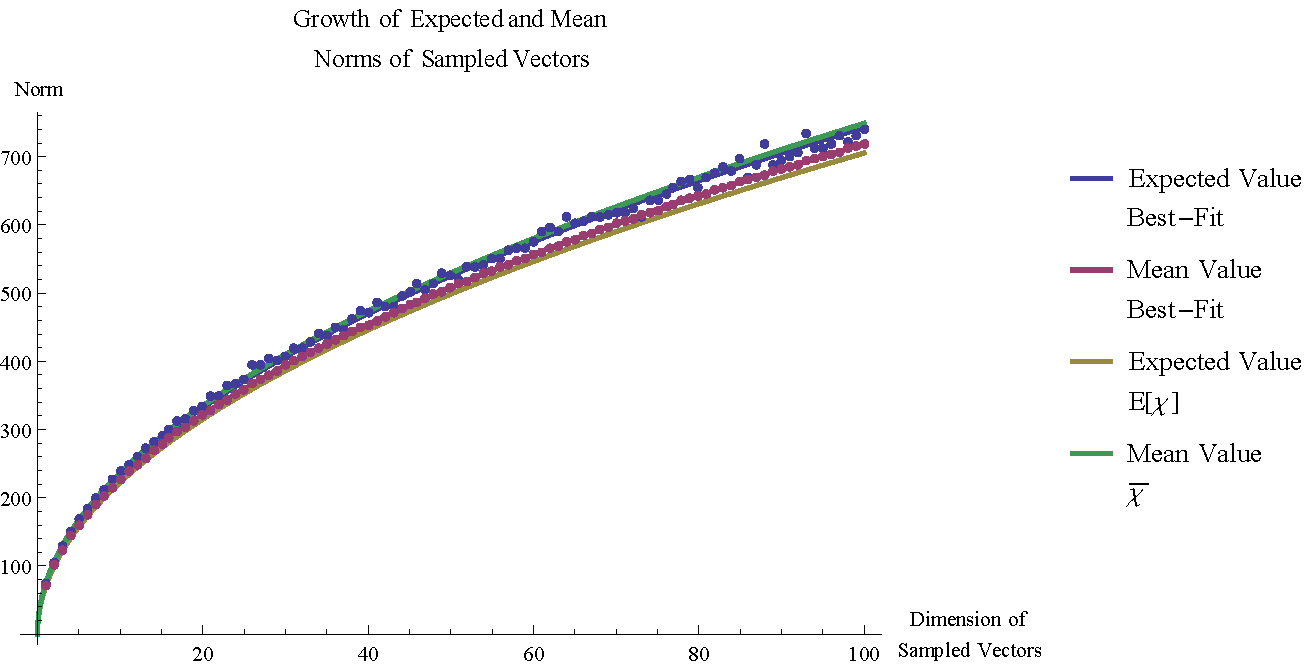
\includegraphics[width=\textwidth]{figures/dnssampling-ev_growth.pdf}
\caption[Growth of Expected and Mean Norms of Sampled Vectors]{The computed
expected and mean values of the norms of the vectors from higher-dimensional
spaces formed by IID observations from the distribution in table
\ref{TABLE_dnssampling} are shown as points. The variation of the expected value from the best-fit
curve is due to the relatively small sample taken from the enormous spaces.}
\label{dnssampling-evgrowth}
\end{figure}

It is important to observe how the various functions compare to the sampled
data. Observe that the best-fit curve for the mean value of the norms of the
sampled data almost perfectly describes the sampled data. The best-fit curve for
the mean values is given by $71.8527\sqrt{n}$ while the yellow curve is given by
$\overline{\chi}\sqrt{n}=70.5263\sqrt{n}$. The marked difference is indicative that $k$ (as in equation
\ref{dnssampling-evgrowth-eq}) is non-unitary. Similarly, the best-fit curve for
the expected value of the norms is given by $74.3039\sqrt{n}$ while the green
curve is given by $E[\chi]\sqrt{n}=74.8797\sqrt{n}$. Note that the best-fit curve in this
situation is subject to much higher uncertainty which may be responsible for
some of the deviation.

In addition to the above, a cumulative density function (CDF) was built from the
sampled vectors and then a function of form given by the CDF of the normal
distribution with mean $\mu$ and standard deviation $\sigma$

\begin{equation}
CDF[N(\mu,\sigma)]=\frac{1}{2} \text{erfc}\left(\frac{\mu -x}{\sqrt{2} \sigma}\right)
\end{equation}

was fit to the data where 

\begin{equation}
\textrm{erfc}(n)=\frac{2}{\sqrt{\pi}} \int_n^{\infty}
e^{-t^2}\,\mathrm dt
\end{equation}

is the complementary error function (used in the CDF of the normal
distribution). Fitting a function of this form to the data allows for an estimation
of the mean and variance of the distribution of the sampled vectors as predicted
by the CLT.

\begin{figure}
\centering
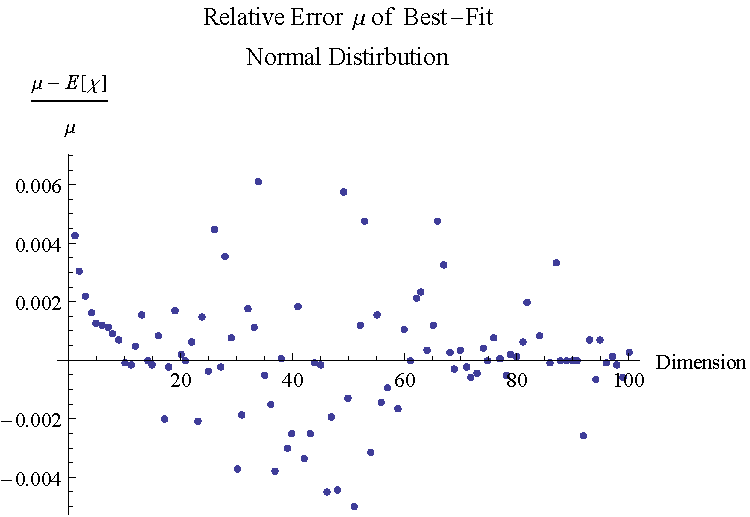
\includegraphics[width=0.7\textwidth]{figures/dnssampling-muerror.pdf}
\caption[Relative Error of $\mu$ of Best-Fit Normal Distribution of Sampled Expected Value]
{For each $n$, vectors were sampled from $\chi^n$ where $\chi$ is given by the
distribution in table \ref{TABLE_dnssampling} and a normal distribution
$N(\mu,\sigma)$ was fit to them. This plot shows the relative error of the
best-fit $\mu$ compared to $E[\chi]$. The trend toward zero for small dimensions
becomes dominated by error due to sampling as $n$ grows.}
\label{dnssampling-muerror}
\end{figure}

\begin{figure}
\centering
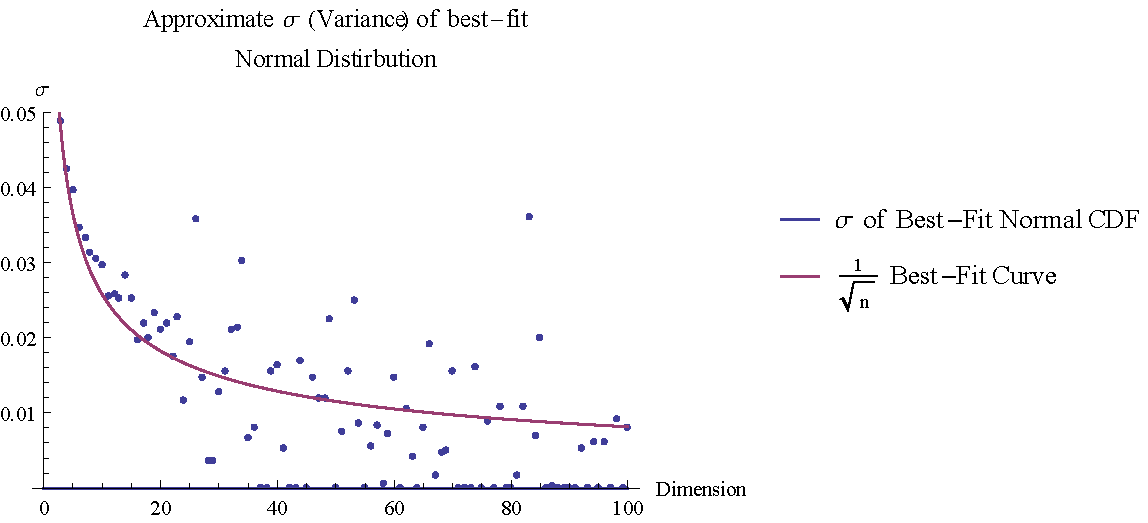
\includegraphics[width=\textwidth]{figures/dnssampling-sigmafit.pdf}
\caption[Trend of $\sigma$ of Best-Fit Normal Distribution of Sampled Expected Value]
{For each $n$, vectors were sampled from $\chi^n$ where $\chi$ is given by the
distribution in table \ref{TABLE_dnssampling} and a normal distribution
$N(\mu,\sigma)$ was fit to their CDF. This plot shows the trend of the best-fit
$\sigma$ as $n$ increases. The trend toward zero for small dimensions becomes
dominated by error due to sampling as $n$ grows.}
\label{dnssampling-sigmafit}
\end{figure}

As is shown in figures \ref{dnssampling-muerror} and \ref{dnssampling-sigmafit}, empirical results show that the theoretical results given in section
\ref{item-four-theory} still hold and are valid for query lengths/dimensionality
within the practical ranges.

\clearpage
\section{Solution Evaluation Criteria}

The objectives that must be met for an
approach to have successfully solved the problem posed in section
\ref{briefproblem} are as follows:

\label{methodreqs}
\begin{itemize}
\item Successfully discern tunnel traffic generated from
existing tunnel applications and theoretical tunnel traffic (built using
additional parameters to attempt to hide from known detection methods) from a
baseline of normal traffic.
\item Be resistant to known obfuscation methods compared to existing detection methods.
\item Be able to operate at high speed on general purpose, easily obtainable
hardware.
\end{itemize}

The proposed approach will be evaluated against these criteria to determine
whether or not it can be considered an improvement on the state of the art for
this type of detection. 

%Items 1 and 3 in the list of criteria require additional
%quantification, however the quantification criteria are different for each of
%the classes of tests. Details will be given in sections \ref{test-existing} and
%\ref{test-weakness} on how detection methods will be scored for their respective
%tests.

Because the implementation of the approaches is built on a Python framework and
is not tuned for high performance, it is not reasonable to set absolute
performance metrics to measure the success of a detection method. Instead, in order to satisfy item 1, a
relative ranking will be applied that examines the performance of the methods
in the context of their peers, all implemented using the same data source and
common Python framework. The framework is described in section \ref{scaffolding}
and the processing performance of the methods is examined in section
\ref{processing-perf}.

Item 2 will be tested using a next-generation tunnel, described in section
\ref{appendix-customdns} and referred to as \texttt{next-gen}, that simulates
what DNS tunnelling applications may look like in the future.

\chapter{Proposed Detection Method}
\label{proposed-method}

The method proposed in this work examines the information theoretical properties
of the DNS queries to each domain, thus retaining the flexibility to filter
and alert per domain as opposed to more generally on the set of all DNS queries.
The tools developed to test this approach utilize full packet data for its
analysis, but can be modified to use name server query logs (as were used in
\cite{Romana2007}) or other sources of query information. The prototype C++ software described in section \ref{cpp-implementation}
is easily capable of running at greater than gigabit speed on inexpensive, off
the shelf hardware making this approach practical and uncomplicated to deploy on
smaller networks or in resource constrained situations. Deployment in large
environments is similarly straight forward.

\section{Theoretical Basis}
\subsection{Assumptions}
The detection approach proposed in this work
makes certain assumptions about the nature of DNS tunnels in order to
effectively detect them. The primary assumption made is that DNS tunnels move
more data than a normal DNS subdomain, with a very particular meaning of
\emph{data} that goes beyond simply counting bytes or the number of queries. The
concept of the amount of data moved under a DNS domain involves considering the
entropy of the queries as a whole, and not the characters that make up a query.
The list of assumptions follows:

\begin{itemize}
\item DNS tunnel applications use the queries themselves to transport data from
the client to server.
\item This mechanism will force there to be more unique
queries per domain (or subdomain) proportional to the amount of unique data transferred
from the client to the server.
\item In a server-to-client transfer of data, there will still need to be
acknowledgements sent from the client to the server, with the acknowledgement
data encoded in the query string.
\end{itemize}

The primary assumption, in the language of DNS queries, is that DNS tunnels will
cause more unique DNS queries to a domain (or subdomain) than benign traffic. If
a DNS tunnel is able to construct its network traffic in such a way that this
assumption is no longer true, then the proposed approach will be ineffective in
detecting it.

\subsection{Theory}
In a large internet provider network, it is possible that there could be many
copies of the same DNS query - say \emph{google.com} - each of which would count
towards the total number of bytes or queries transferred to/from that domain. If a naive
approach to detection is used, such as counting bytes or queries to/from a
domain, then this kind of repetition will have a detrimental effect on the
metric calculated for some popular domains.

In order to work around this, the proposed approach takes a different stance on
unique data and instead uses entropy to measure the amount of data moved in the
queries to a domain or subdomain. By considering queries as atomic objects, and
maintaining a tally of the queries to a domain, and their counts over an
interval, a probability distribution function (PDF) is generated. By computing
the entropy of this PDF, a basic measure of throughput is achieved. However,
since there is value in the capturing the length of the queries that were sent
(since longer queries are moving more bytes than shorter ones), the entropy is
multipled by the average query length (in bytes) over that interval.

This metric, which will be referred as the Domain Length-Weighted Entropy
(DLWE), is the primary mechanism through which the proposed approach detects DNS
tunnels.

With this new measure of data, the approach considers intervals of time and
computes the amount of data estimated to be moved by each domain over that
interval. By sorting all domains by their data throughput, the heavy-hitters can
be examined in each time interval with white-listing preventing many of the top benign
contenders from causing alerts.

As will be shown in chapter \ref{chap-evaluation}, this approach is capable of
processing packets nearly as fast as a naive approach with equivalent or better
detection performance.

\section{Implementation}
\label{implementation}
\subsection{General}

The implementation specifics of this approach differ slightly between the C++
and Python implementations. The differences come primarily in efficiency and
performance of the approach, with the C++ implementaiton designed for very high
throughput applications. Both implementations, however, share a common
architecture:

\begin{itemize}
\item The input is DNS queries and a timestamp at which the query was seen
\item The DNS query is broken down into a top-level domain (TLD) - such as
\emph{google.com}, \emph{yahoo.ca} or similar - and the rest of the query - such as \emph{www} in \emph{www.google.com} and \emph{plus} in \emph{plus.google.com}.
\item For each TLD, a data structure is created that maps queries
to an integer, which represents the number of times that query was seen.
\item At the end of each time interval, the DLWE of each TLD is calculated, and
the collection of TLD+DLWE pairs is output.
\end{itemize}

\subsection{C++}
\label{cpp-implementation}
The C++ implementation ingests raw packet data in the PCAP file
format, relying on a purpose designed network protocol dissector for the
extraction of the DNS query string, TLD, and any response information. The query
timestamps are obtained from the packet header which is part of the PCAP format.

The data structure used for storing the query-count mappings for each TLD is a
custom high-performance, low memory usage, red-black tree written as part of
libodb\cite{Friesen2013}. Computation of the DLWE for each TLD at the end of
each interval is handled asynchronously in a separate thread so as not to block
the ingestion of packets on the main thread. This asynchronous behaviour allows
the processing to operate on very busy networks and allows for inherent and
elegant non-blocking buffering of bursts of traffic beyond the processing rate
of the host.

The C++ implementation is capable of processing in excess of four hundred
thousand packets per second on commodity quad-core CPUs from 2011. The source
code is included in the libodb source code distribution\cite{Friesen2013}.

\subsection{Python} The Python implementation details are described in section
\ref{proposed-method-python}.

\chapter{Detailed Testing Methodology}
A collection of tests will be run on
several detection methods, demonstrating the performance of this work's proposed
method when compared to existing methods from the literature. The detection
methods chosen for comparison is composed of

\label{chosen-methods}
\begin{itemize}
\item The $n$-gram detection proposed by Born\cite{Born2010.cfa} because it is
well defined and was the most prevalent approach found during the literature
search.

\item The use of \emph{gzip} on domain and subdomain packet data as proposed by
Paxson\cite{Paxson2011} because it involves looking at data that is very similar
to the approach outlined in section \ref{implementation}, but makes use of
different methods for measuring the data throughput.

\item A naive approach that simply measures the volume (in number of characters
in the query strings) of packets per domain/subdomain in an attempt to illustrate that simple
volume of queries is a highly inadequate approach, and that more sophisticated
approaches can perform considerably better.
\end{itemize}

The collection of methods will be put through several tests in an attempt to
demonstrate their performance in average (using existing implementations) and
worst case scenarios. All of the tests involving traffic generation will be
performed in a virtual environment of two linux-based virtual guests directly
connected via a virtual network on a single physical host.
%, with technical configuration and testing
%details given in section \ref{appendix-setup}.

\section{Situational Performance Goals}
\subsection{Determining a Baseline}
\label{baseline}
Through cooperation with Merlin, an educational internet service provider (ISP)
in Manitoba, DNS traffic was collected over a period from Thursday November 4
2010 until Friday November 26 2010. The hosts responsible for the DNS traffic
observed include several dozen school divisions totalling tens of thousands of
individual computers. The capture includes just over one billion packets
destined to, or sourced form, UDP port 53 (the standard DNS port). Not all
packets are valid DNS with more detailed information on the properties of the
sample available in appendix \ref{appendix-capturestats}.

This captured traffic will be used to determine a baseline distribution to which
the metrics produced on isolated tunnel traffic can be compared. This baseline
will provide context in order to determine if a method is able to detect a
tunnel with sufficiently high certainty.

It is assumed that the incidence of tunnels in this baseline traffic is
sufficiently low that it can be discounted. This assumption may not be perfectly
accurate due to to reasons indicated in the introduction. Because many security
vendors use DNS to transmit some of their information, these transmissions are
in essence a DNS tunnel and so will represent a certain portion of the real
world traffic. The effect of tunnels present in the real world traffic given the
assumption that there are none will result in a more pessimistic environment for
testing. Since some of the traffic that is lies further out than the synthesized
traffic, a portion of the ambiguity that the detection approaches will suffer
may actually be due to the classification of existing traffic as a tunnel, and
not due to misclassification.

%This capture of DNS traffic will be used to determine the baseline behaviour of
%normal, benign DNS domains such as \texttt{google.com}, \texttt{yahoo.com}, and
%other large commonly used domains. This dataset will also be used to give
%context to the results obtained by the detection approaches when run on the
%synthetically generated tunnel traffic. It is important to note that even if one
%method picks out the synthetic tunnels more clearly than others, all that
%matters in the end is that the tunnels are distinguishable from the background
%noise of normal traffic.

\subsection{Existing Implementation Detection}
\label{test-existing}
This test will involve the two hosts communicating at varying throughput rates
using the chosen existing DNS tunnel implementations. The throughput rates will scale
from as little as several bytes per second, to several megabytes (or as high as
the tunnel applications can support) per second. The wide range of throughputs
used is done to give an indication of how the detection methods scale with
tunneled throughput.

The existing implementations chosen for testing in this section are
Iodine\cite{iodinesrc}, DNScat\cite{dnscatsrc}, and DNS2TCP\cite{dns2tcpsrc}.
Iodine is chosen due to the fact that it provides a full VPN solution without
additional work by the user. DNScat is chosen due to being written in Java and
so runs on multiple platforms\footnote{DNScat will run on any platform that
supports Java 1.4 or later\cite{dnscatsrc}} without the need for a compiler or
other complex dependencies that the user must obtain. DNS2TCP is chosen since it
does not require root access, and is written in C indicating potentially better
throughput than other mechanisms.

The detection results of each of the approaches on the existing tunnelling
applications is of value to those wishing to identify uses of DNS tunnelling
currently in the wild. Because the tests do not involve distinct events that
will be detected (or not), but rather a much smaller number of prototypical
events, false-alarm and false-negative rates are not necessarily the most
instructive indicators. Because of this, each detection method will be have a
\emph{minimum certainty of detection} assigned to it for each type of tunnel.
Details of how this certainty is calculated is given in section
\ref{tunnel-detection-performance} as well as the certainty values for each
detection method for the various tunnelling applications. Intuitively, however,
the certainty can be thought of as, given the distribution of metrics for normal
traffic and a new measurement for comparison, the probability of making the
correct determination as to whether or not measurement represents a tunnel.

This certainty indicator will give a rough estimate of the effectiveness of the
detection algorithms in the various tests. A certainty greater than 0.90
represents a moderate level of success, and a certainty greater than 0.95
indicates a high level of success.

\subsection{Demonstration of Existing Weaknesses}
\label{test-weakness}
The tests in this section will demonstrate that the weaknesses listed in section
\ref{litreview-summary} are in fact exploitable by software and are not simply
theoretical in nature. For the purposes of this section, a new type of tunnel
was simulated using a tool that generates queries according to potentially more
complicated rules that would be difficult to integrate into existing solutions.
The implementation details for this tool are given in section
\ref{appendix-customdns}.

As in section \ref{test-existing}, the certainty indicator will be used to
evaluate the efficacy of the detection methods on this more advanced type of
traffic.

\subsection{The Effect of DNS Caching on Detection Effectiveness}
Because the packet capture was done in an environment where a large portion of
the clients use one of only a few different DNS servers, the effects of caching
will cause the naive approach to have higher detection performance than if this were not the case. If this were
an environment such as a large ISP or internet backbone where such DNS caching
is not present then the naive approach will have far different detection
performance and characteristics. Unfortunately, due to the nature of the network
capture obtained for this work, it is not possible to demonstrate how the naive
approach performs in a uncached DNS environment.

In order to grant some possible context to the effects that DNS caching has had
on the naive method's performance, a simple comparison is offered. Data was
taken from a home network serving five computers and smartphones, with DNS
traffic logged over a twenty-two day period to match the time frame of the
capture for real world data. Over that twenty two day period,
\emph{www.google.com} was queried 5645 times compared to the 268842 times the
same query was seen in the real world traffic capture. It is important to modulate these
values by the number of hosts that the real world traffic represents, which
is on the order of approximately thirty thousand, or six thousand times the
number of hosts the home network was supporting.

Approximately scaling the home network by a factor of six thousand results in an
estimated three million queries to \emph{google.com} occurring in the real world
traffic, of which only a twelfth actually appeared in the capture due to
DNS caching. This is only one common domain name, so applying similar logic to
other domains, it is easy to see that in these scenarios, the normal curves
would take on a very different shape, easily obscuring tunnel traffic for low
throughputs.

A small sample of data was collected from Merlin's caching DNS servers which
represents \emph{every} DNS query made of them, regardless of whether those
queries were served from the cache or not. This type of DNS sampling presents a
high load on their instrumentation infrastructure, and so is only reasonable for
this type of comparison. The logs obtained from their servers span four hours
from 1200 to 1600 on a Thursday afternoon. Figure \ref{caching} shows the DNS
query logs from Merlin's servers, the home network's DNS query logs, and the
queries from the packet capture and their counts. As can be seen from the plot,
which is logarithmic in the vertical axis, shows that, on average, the queries
in an uncached environment occur over two orders of magnitude more frequently
than in a cached environment. This increased occurrence in an uncached
environment would have a strongly visible impact on the naive metric's ability
accurately detect DNS tunnels.

\begin{figure}[h]
\centering
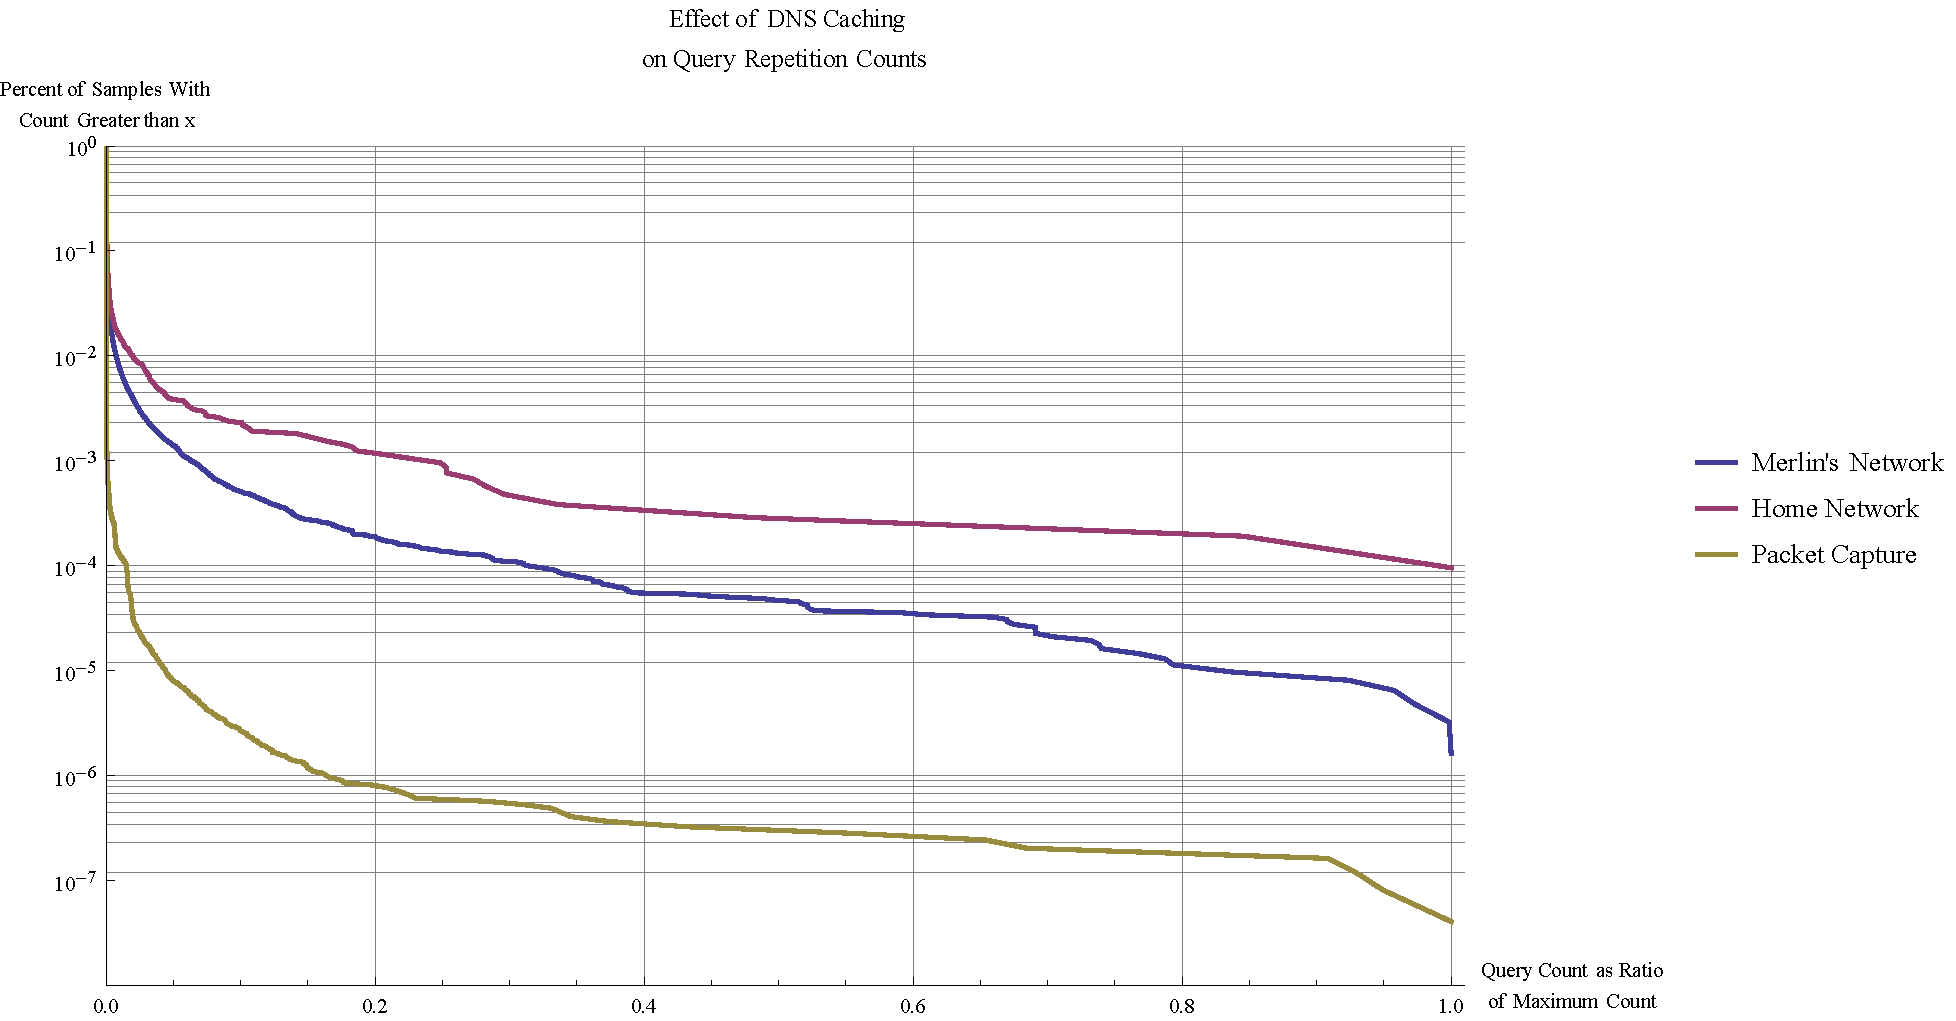
\includegraphics[width=\textwidth]{figures/caching.pdf}
\caption[Effect of DNS Caching on Query Counts]{Shows the trends for DNS query
counts in networks with and without caching. The axes are normalized to account
for the fact that the real world data has much more data than the home network.
By normalizing the query counts, it is possible to perform a direct comparison.}
\label{caching}
\end{figure}

As can be seen from the proposed method's underlying mechanisms, the DNS caching
actually provides a \emph{more pessimistic} detection environment compared to
the uncached environment. Unlike the naive method, whose detection performance results
will not be applicable in an uncached environment, the proposed method can
be expected to perform better in an uncached environment than they do in the
testing in section \ref{detection-perf}.

Born's method will also improve in detection performance in an uncached network,
since it will cause normal traffic to have a character distribution more heavily
skewed away from uniform, resulting in larger metrics and better certainty.
Paxson's metric, however, will suffer in an uncached environment due to the fact
that additional data, even it is highly repetitive, will still increase the
metrics of normal traffic and may obscure some DNS tunnels in the process.

\section{Analysis Method Implementations}
\label{implementations}
\subsection{Common Scaffolding}
\label{scaffolding}
All implementations of the analysis methods are built on the same basic
framework written in Python. The framework has the following basic properties:

\begin{itemize} \item Unlike the C++ implementation of the proposed approach
described in section \ref{cpp-implementation}, which ingests raw PCAP formatted
data, the Python scaffolding is unable to do so. Instead, the Python scaffolding
relies on another tool to process raw packet captures (or other data sources
such as DNS server logs) into a comma-separated value (CSV) file with a
timestamp and a query strong on each line.

\item The scaffolding takes in two arguments: a file name to read the
timestamp/query pairs from, and how long the intervals should be, in seconds.

\item At the start of each interval, the main loop initializes an array to hold
all of the queries for the upcoming interval. For the duration of the interval,
the queries are added to the end of the array, which is passed to the analysis
routine (where the specific detection method details are) at the end of the
interval.

\item When the queries from the interval are handed off for processing, each
query has its top-level domain (TLD) identified, and then the rest of the query
is passed to the specific method. The returned value is then assigned to the TLD
that the query came from.

\item Once processing of the interval is complete, the array is cleared in
preparation for the beginning of the next interval.

\end{itemize}

There are some very important differences between the C++ implementation and
this Python scaffolding that will cause the performance metrics to not be
directly comparable.

Unlike the C++ implementation which is designed for maximum performance and
non-blocking ingestion of traffic, the Python implementations are poorly behaved
around the ends of intervals where ingestion stops while processing occurs.
Additionally, there is a reliance on another tool to produce the appropriate 
input data. This removes the complexity of
parsing and verifying the packet protocols from the performance figures for
these implementations.

\subsection{Naive}
\label{implementation-naive}
The metric returned for each query (stripped of its TLD) is simply the number of
characters in the query. For each TLD, after all of the packets are processed,
the total of all of the metrics for each query are summed together resulting in
a single value that counts all of the characters that appeared in queries to
that TLD.

\subsection{Born}
%Since the technique proposed by Born relies on having a notion of normal
%traffic, a PDF of the character frequencies from the Alexa top one-million
%domains was built (as is given in tables \ref{TABLE_dnssampling}) as the
%baseline of normal. Additionally, this PDF was sorted from most to least
%frequent character since the method relies on the assumption that DNS queries
%approximately follow Zipf's Law, and not that they match the exact character
%frequencies.

Since Born's\cite{Born2010.cfa} assumption is that normal DNS queries
approximately follow Zipf's Law, and that tunnels produce character
distributions that are much closer to uniform, this was used to determine a
metric. At the end of each interval, for each TLD all of the queries to that TLD
are taken together and joined into a single long string. The character
distribution of that string is then computed, and its standard deviation
calculated.

Since it is expected that tunnel traffic is close to uniform in its character distribution, it is then assumed
that tunnels will have a very low standard deviation while normal queries will
have a standard deviation that increase very quickly by comparison.

Because the next-gen tunnel (as described in section \ref{appendix-customdns}) used in the tests is designed to circumvent Born's
detection method (any any other method that relies on character frequency
analysis), it is expected that this approach will have poor detection
performance on the next-gen tunnel.

\subsection{Paxson}
Paxson's\cite{Paxson2011} approach uses the \emph{gzip} utility to compress the
queries to domains under the assumption that it will approximately measure the
amount of unique data contained in those queries. Because \emph{gzip} is a
command line interface to the underlying \emph{zlib} library, in Python this
approach was implemented by making calls to Python's \emph{zlib} library and its
\texttt{zlib.compress()} function.

As with the previous implementations, the queries for each TLD over an interval
are accumulated and joined together into a single long string. This string is
then passed to the \texttt{zlib.compress()} resulting in a string whose length
becomes the metric for that TLD in the current interval.

Because Paxson's approach uses very similar assumptions, that DNS tunnels can be
detected by measuring the amount of unique data transferred to each domain
and/or subdomain, it is expected that Paxon's approach and the proposed approach
will have very similar detection performance. However, due to the fact that
Paxson's approach relies on a general-purpose compression library whereas the
proposed approach uses a tailored algorithm and optimized data structures, it is
expected that the proposed approach will have superior processing performance.

\subsection{Proposed Approach}
\label{proposed-method-python}
In place of the high-performance red-black tree used in the C++ implementation,
a Python \texttt{dict} was used in the Python implementation. The \texttt{dict}
is used as a mapping from query strings (with the TLD removed) to integers
indicating how many times that string appeared in the interval. At the end of
each interval, such a mapping is built for every TLD from the packets seen in
the interval, and for each TLD, the DLWE is computed from the obtained
distribution. The computed DLWE is then used as the metric for the TLD for that
interval.

\subsection{Tunneling Application Throughput}
\label{tunapptp}
The tunnelling applications used during the evaluation were subjected to
different rates of traffic in both client-to-server and server-to-client
directions. For each tunnelling application, sixteen captures were performed at
each of the following target throughput rates (in bytes per second):

10, 25, 50, 100, 250, 500, 1000, 2500, 5000, 10000, 25000, 50000, 100000,
250000, 500000, 1000000

Due to implementation details of the applications, and of the next-gen tunnel,
not all applications were able to transmit traffic at the target rate. Figure
\ref{tunrates} shows how the various tunnelling applications responded to
various input rates, plotting their actual rate of ingestion of input and the
observed number of characters of query output they generated on the network. Note
that for the lighter coloured graphs showing the observed output, the vertical
axis is representing a value equivalent to the naive metric. The next-gen tunnel
was not tested in a server-to-client direction.

\begin{figure}
\centering
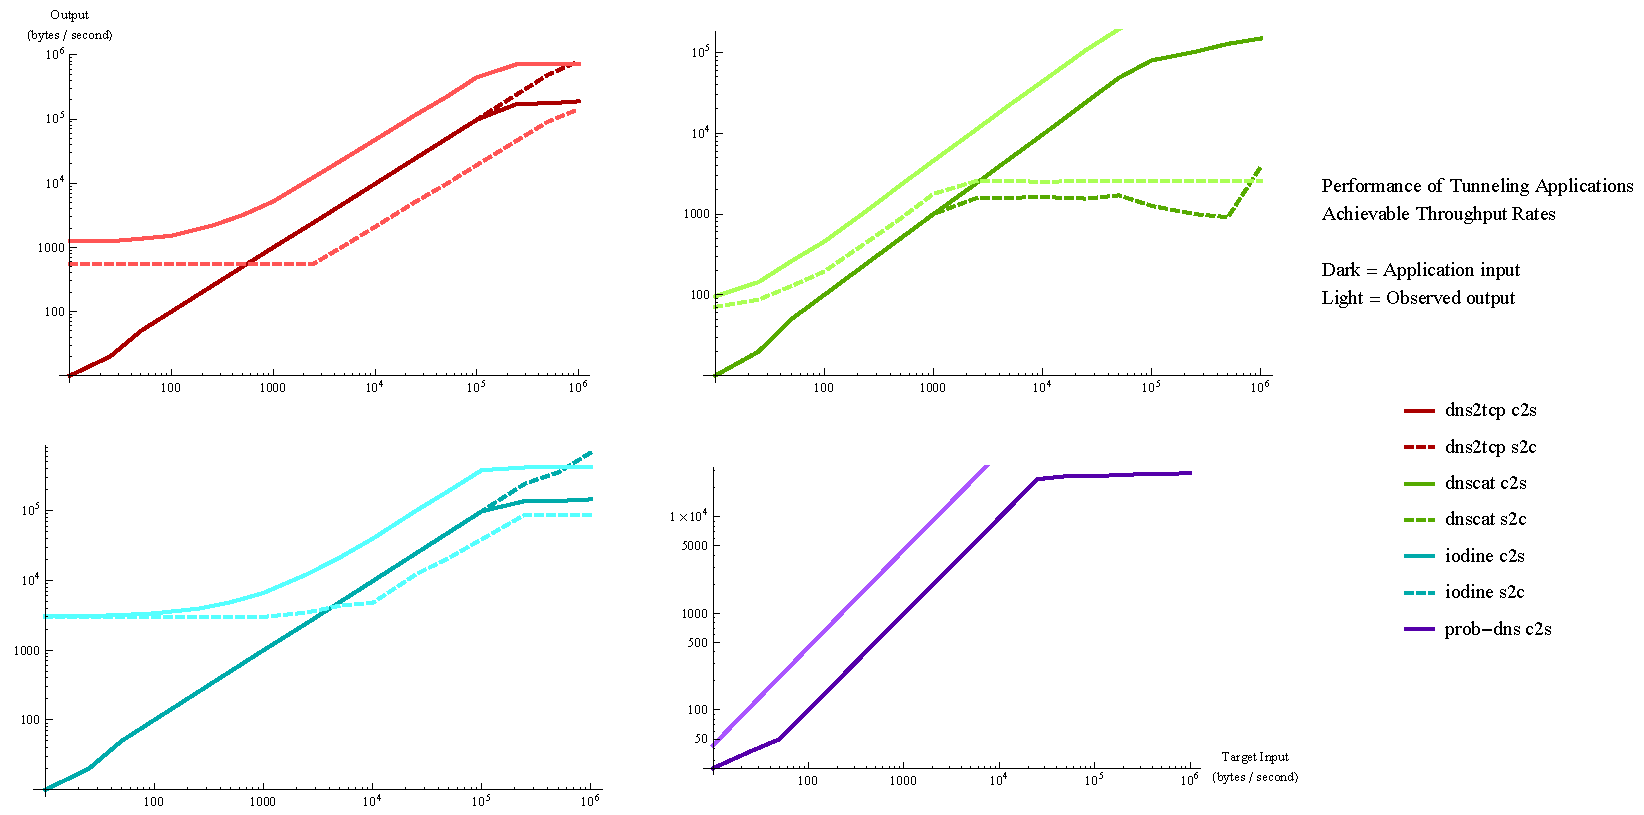
\includegraphics[width=\textwidth]{figures/tunrates.pdf}
\caption[DNS Tunneling Application Throughput Scaling]{Shows the scaling
behaviour of DNS tunnelling applications as the input rate is scaled up. Note
that not all applications are capable of transmitting data at the rate they are
given data, which is visible as a plateau on the right-hand-side of each plot.}
\label{tunrates}
\end{figure}

\subsection{Detection Method and Python Interpreter Processing Performance}
\label{processing-perf}
Python has several interpreters available freely in addition to the standard
interpreter (for this discussion, the standard interpreter will be referred to
as Cython). A notable alternative, called PyPy, is a Python interpreter written
in Python itself that contains just-in-time compilation (JIT) mechanisms that
Cython does not have. The advantages of JIT compilers and interpreters include
being able to dynamically optimize heavily used code paths based on run-time
statistics and information that would not otherwise be possible in a static way
at compile-time. Because of this advantage, PyPy can offer an order of magnitude
or better speedup\cite{pypyvc-strfmt} in some workloads.

Because of this potential advantage, PyPy was investigated as an alternative to
Cython when performing the analysis with the Python-based implementations of the
detection algorithms. Figures \ref{pmat}, \ref{pmqr}, and \ref{pmqr-100k} show
the performance of the various detection methods over aggregate tunnel and
real-world data.

Figure \ref{pmat} shows that the analysis methods under Cython all suffer, to varying
degrees, as the amount of data to process per interval increases. The naive and
proposed methods suffer the least, while Paxson's method suffers by far the most,
dropping to approximately half of its original processing rate. Note that the
Born's method and Paxson's method trade places as the slowest performer at a
throughput of approximately five kilobytes of data per second.

When looking at
the PyPy performance, with the exception of a dip around one kilobyte of data
per second, performance increases as the amount of data increases in direct
contrast to the behaviour of Cython. This increase in performance can be due to
the JIT components having enough time to achieve some measurable optimizations
of common code-paths. In addition, the general ranking of the algorithms by
performance is maintained (with the exception of the swap of Born and Paxson
seen under Cython) from Cython to PyPy. Despite this improvement, the average
performance is still nearly an order of magnitude below that of Cython in many
of the cases.

\begin{figure}
\centering
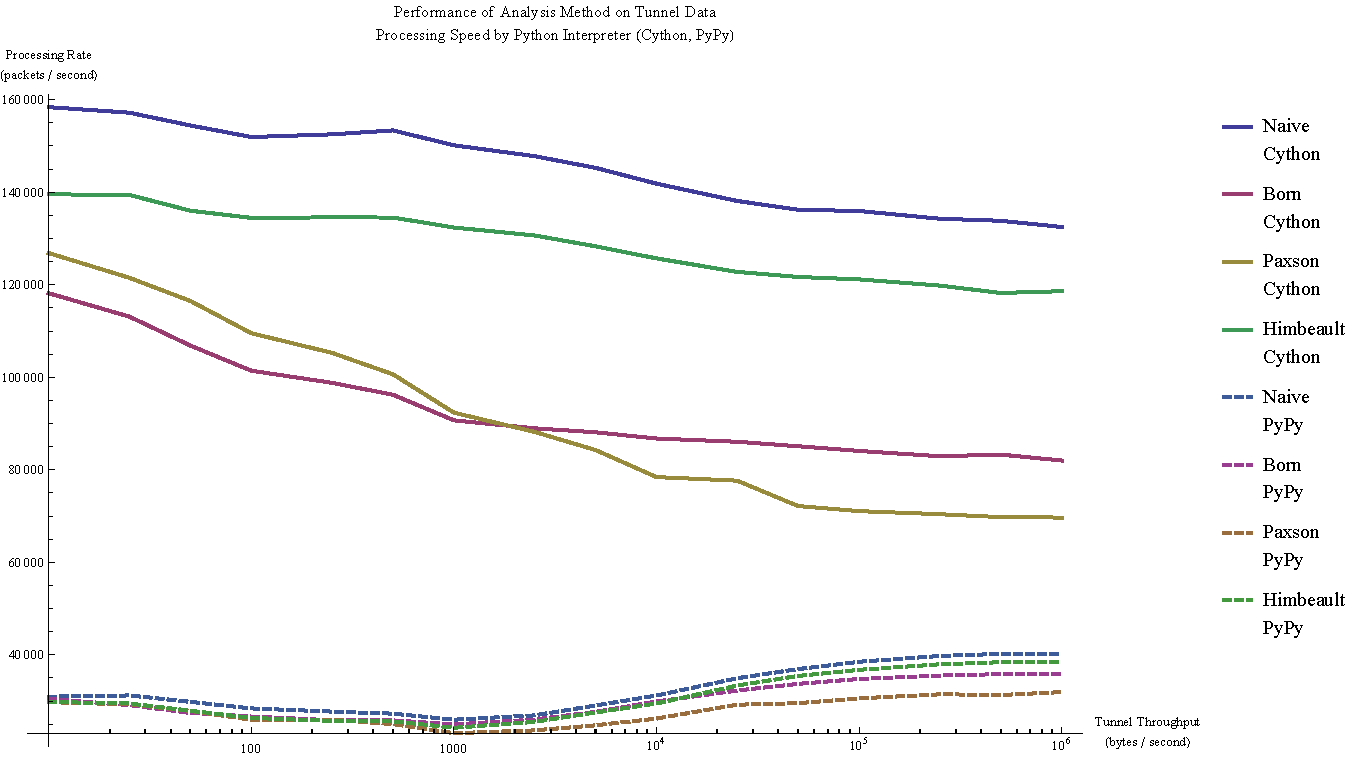
\includegraphics[width=\textwidth]{figures/pmat.pdf}
\caption[Performance of Analysis Method and Python Interpreter on Aggregate
Tunnel Data]{This plot shows the performance of the detection methods and Python
interpreters over the aggregate tunnel data. The output is packet processing
rate as a function of the target input rate (rate at which the tunnels are
transmitting traffic). As the target input rate increases, the structures
involved in the methods get larger in a non-linear way, resulting in longer
operation times and slower performance.}
\label{pmat}
\end{figure}

Figure \ref{pmqr} shows the performance over time of the different detection
methods and Python interpreters as more packets are ingested. Observe that as
the time progresses, the methods get progressively slower, likely due to
inefficiencies in the interpreter and/or method. Again, the naive method is the
fastest, with the proposed method performing at approximately two thirds of the
speed of the naive method. Unlike with the aggregate tunnel data, no swapping of ranks between
Born's and Paxson's methods is observed.

Also unlike the aggregate tunnel detection performance, the methods when run
under PyPy perform \emph{far} better, even surpassing the Cython counterparts in
at least one case. Note that the Paxson's approach when run under PyPy shows
decreasing performance over time while no such decrease for larger times is
observed when run under Cython. PyPy out-performs Cython when performing Born's
approach by a considerable margin beginning very early on. A much smaller
performance difference is witnessed between the two interpreters for the
proposed method, with PyPy out-performing Cython by a small margin near the end
of the sample data.

\begin{figure}
\centering
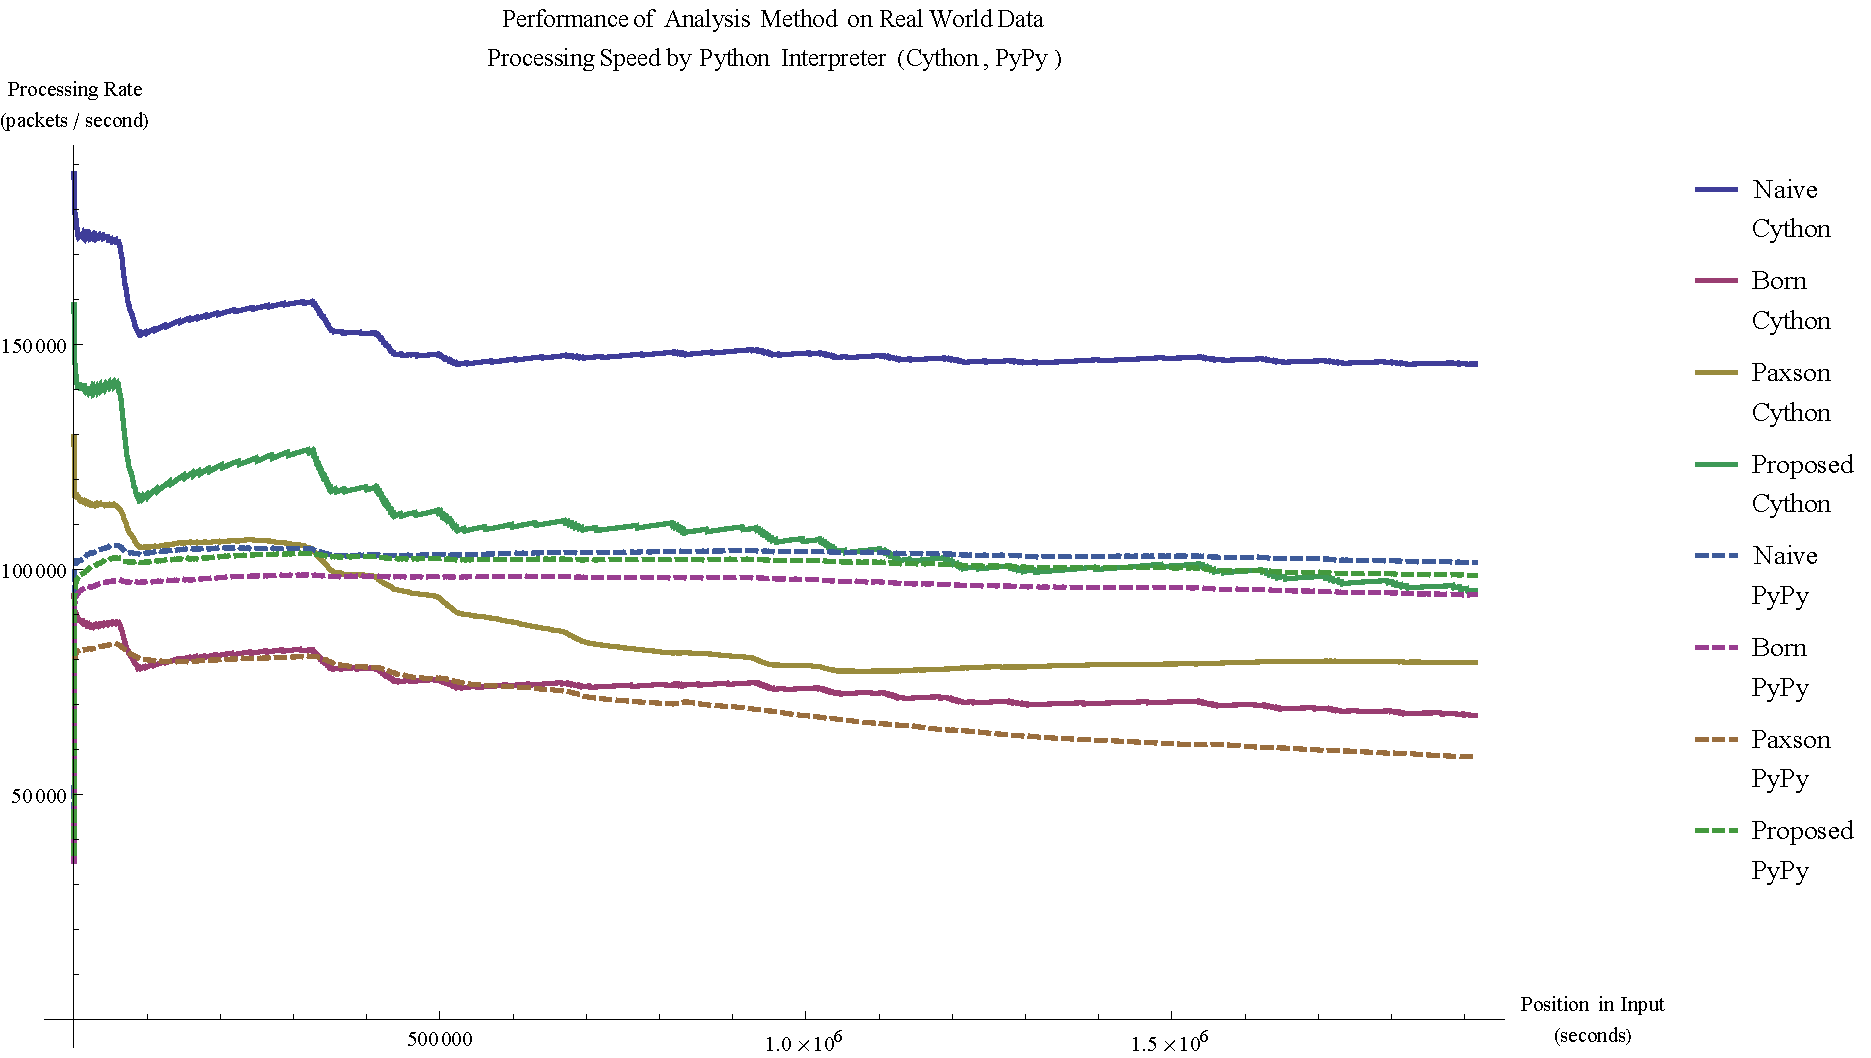
\includegraphics[width=\textwidth]{figures/pmqr.pdf}
\caption[Performance of Analysis Method and Python Interpreter on Real World
Data]{This plot shows the performance of the detection methods and Python
interpreters on real world DNS traffic. The output is packet processing performance as time
progresses and more packets are processed by the script. As more packets are fed
into the script, inefficiencies in the methods and/or the Python interpreters
themselves become observable in the degradation of performance.}
\label{pmqr}
\end{figure}

Figure \ref{pmqr-100k} shows the same data, but with a limited scale allowing
early-time behaviour to be examined. Note that the ramp-up of PyPy's JIT
components is observed in the very early time followed by a very consistent
processing rate. PyPy's processing rate, as show in \ref{pmqr} can be seen to be
far more consistent and not subject to the same degradation and spikes as when
run under Cython. This difference in behaviour indicates that the issues
observed under Cython are likely related to Cython and not the implementation,
since both PyPy and Cython use the same source code files defining the detection
methods.

\begin{figure}
\centering
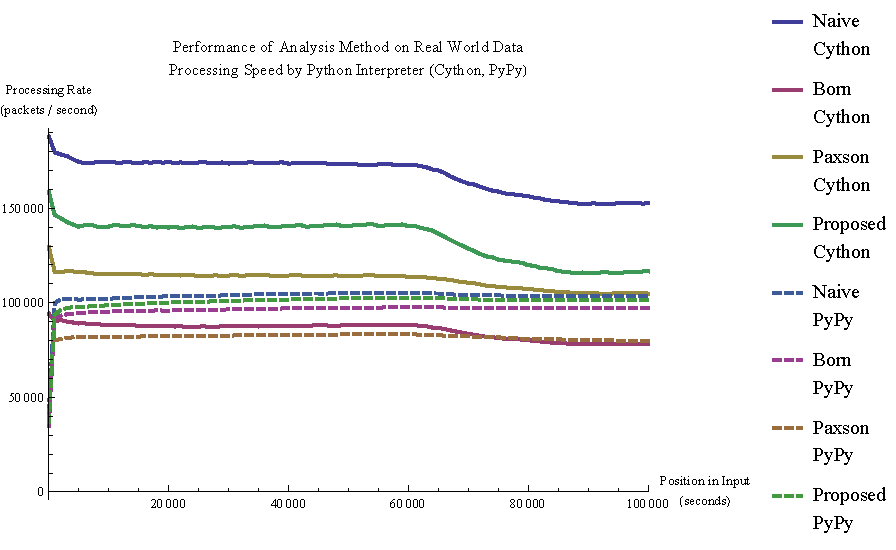
\includegraphics[width=\textwidth]{figures/pmqr-100k.pdf}
\caption[Performance of Analysis Method and Python Interpreter on Real World
Data - Early Time]{This plot is identical to figure \ref{pmqr} but restricts the time
displayed to the first one hundred thousand seconds. The 'spool up' of the JIT
portion of PyPy is noticable in the very early time-scales.}
\label{pmqr-100k}
\end{figure}

Figures \ref{ppia-born}, \ref{ppia-naive}, \ref{ppia-paxson}, and
\ref{ppia-proposed} attempt to represent the performance of the various
detection methods and Python interpreters as more tunnel data is moved through
them per interval. Their horizontal axes are their data input rate (actual data
input rate is used, instead of target input rate, due to the performance
characteristics discussed in \ref{tunapptp}), and the vertical axes indicate the
processing rate (in packets per second) of the approach on the two Python
interpreters (Cython and PyPy).

In the above mentioned figures the legend requires some additional context. The
plot legends contain labels of the form \emph{dns2tcp c2s Cython} which contains
three distinct pieces of information. The first word indicates which tunnelling
application being one of DNS2TCP, DNSCat, Iodine, or the application described
in \ref{test-weakness} which is indicated by a name of \texttt{next-gen}. The
second word indicates whether the data being moved over the tunnel is being
transferred from the client to the server (\texttt{c2s}) or from the server to
the client (\texttt{s2c}). The final word indicates which Python interpreter is
being used.

There are fourteen lines on each figure, each corresponding to a Python
interpreter, tunnel application, and data transfer direction triple. The solid
lines correspond to runs made under the Cython interpreter and dashed lines
indicate the use of the PyPy interpreter.

\begin{figure}
\centering
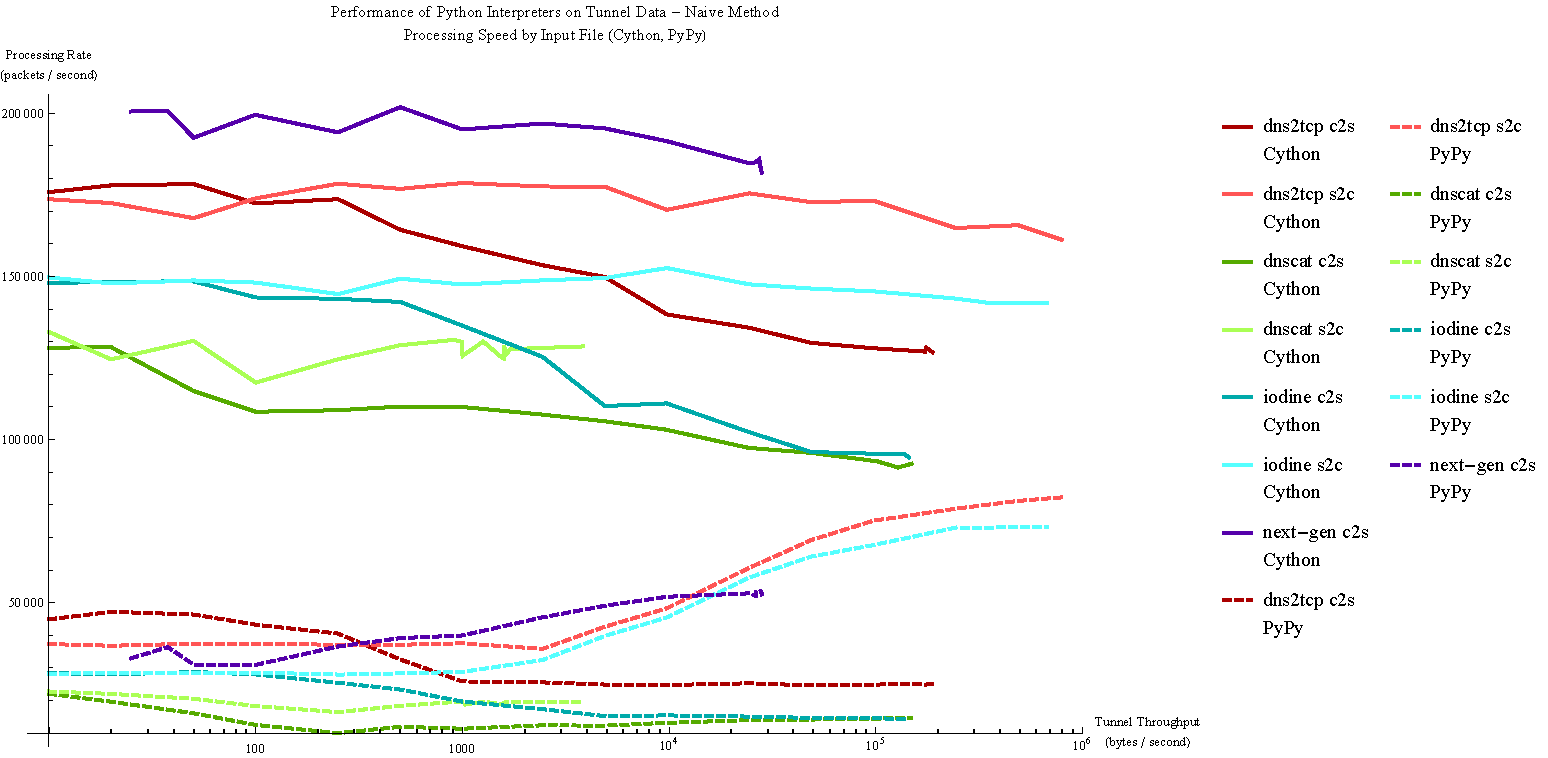
\includegraphics[width=\textwidth]{figures/ppia-naive.pdf}
\caption[Performance of Naive Method on Tunnel Data by Python
Interpreter]{Performance of the naive method on separated tunnelling application
data, showing processing rate as a function of input rate.}
\label{ppia-naive}
\end{figure}

The performance of the naive method has very little dependence on the input
rate, suffering minimally as the amount of data per interval increases. This is
expected behaviour since Python's string objects allow for efficient computation of
length, being of $O(1)$ computational complexity\cite{python-strlencplx}.
Because the naive method's implementation must calculate the length of each
query, additional queries increase the time complexity of the method linearly
with the number of queries that must be processed. The Iodine and DNS2TCP
client-to-server transfers show marked drops in performance, potentially due to
longer queries being used which would increase the time taken to read the files
into the script.

The PyPy performance figures show similar clustering to the Cython plots, with
the notable exception that the DNS2TCP and Iodine server-to-client performance
improves drastically for higher throughputs. This is again likely due to the JIT
components of PyPy being able to optimize for runtime conditions. Despite this
improvement, they still perform at approximately half the rate of their Cython
counterparts at the most favourable throughputs.

\begin{figure}
\centering
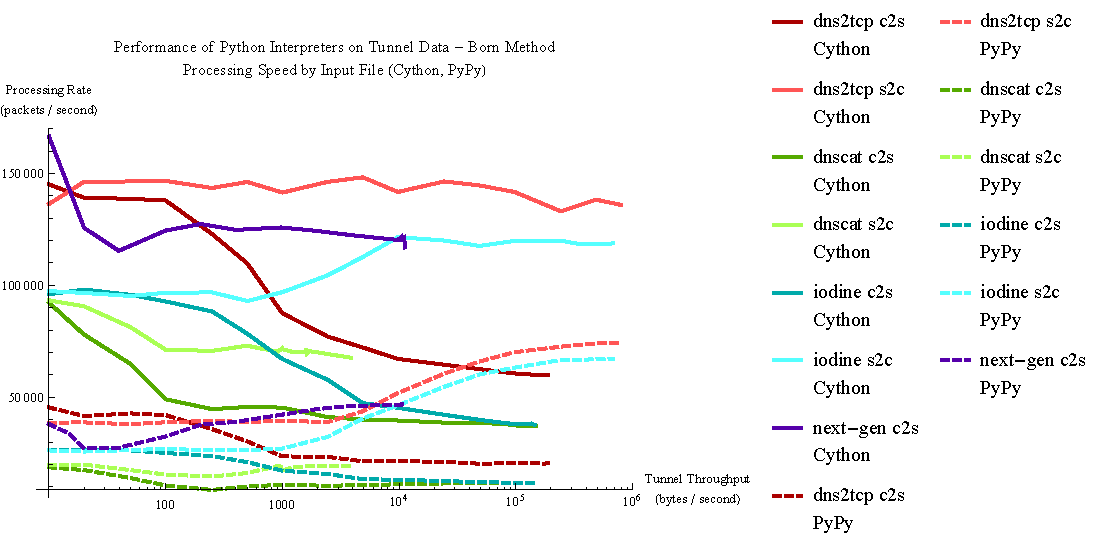
\includegraphics[width=\textwidth]{figures/ppia-born.pdf}
\caption[Performance of Born's Method on Tunnel Data by Python
Interpreter]{Performance of Born's method on separated tunnelling application
data, showing processing rate as a function of input rate.}
\label{ppia-born}
\end{figure}

Born's approach shows a very high level of variation in performance, with marked
decreases in processing rate as the throughput is increased for many of the the
tunnel applications. Notable exceptions are the Iodine and DNS2TCP
server-to-client transfers which suffer minimal degradation or improve as
throughput increases respectively. Again, the same patterns as with the naive
approach are seen under the PyPy runs, however relative performance overall is much
better from PyPy. This is in part due to the much larger performance hit taken
by the Cython implementations. This performance is likely due to the fact that
the Python implementation of Born's approach makes use of a collection of loops
and arithmetic. This type of computation is not well optimized under Cython but
can be subject to excellent run-time optimization under PyPy's JIT components.
PyPy is still, however, unable to improve upon, or match, Cython's performance in these
workloads.

\begin{figure}
\centering
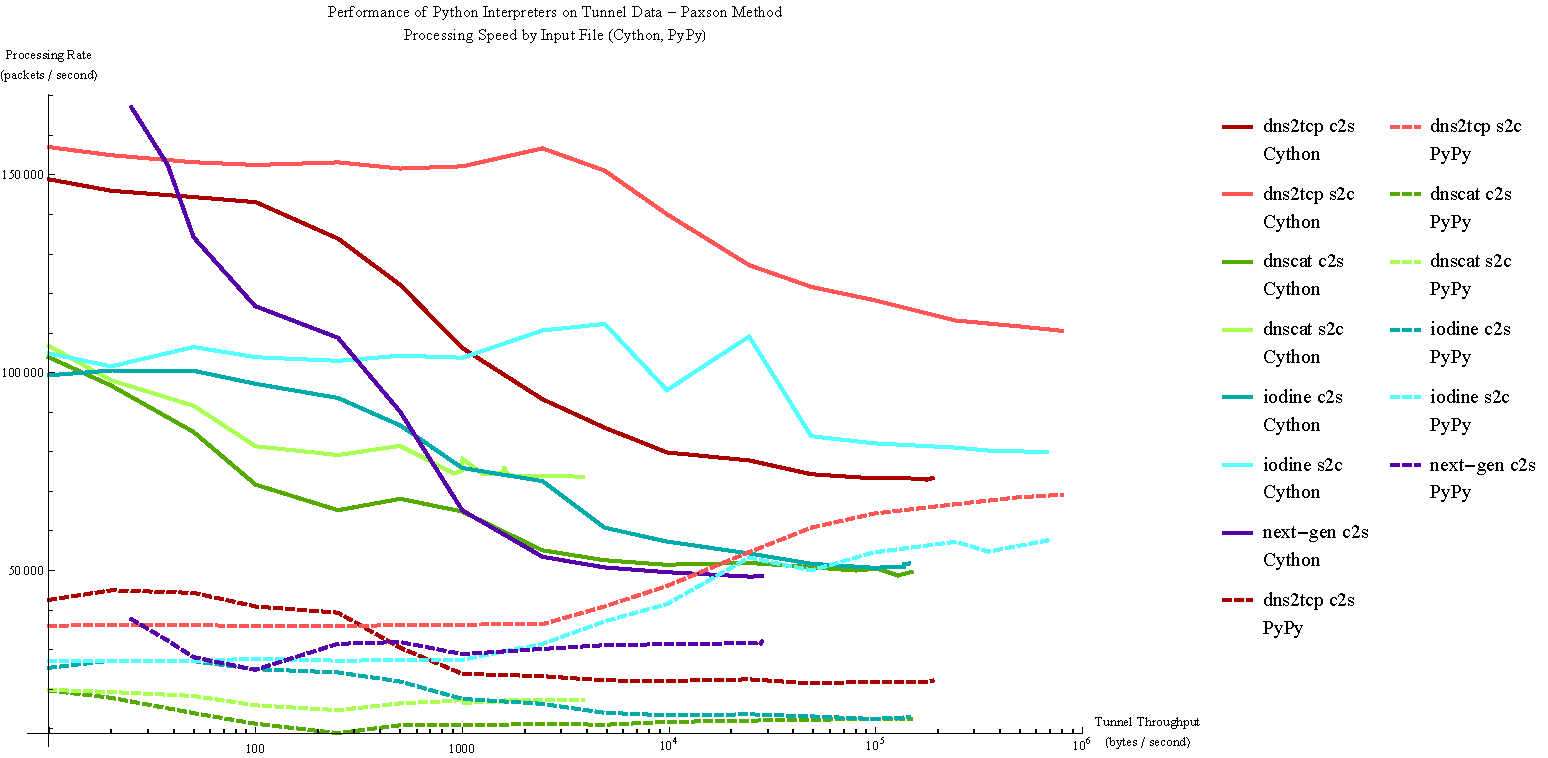
\includegraphics[width=\textwidth]{figures/ppia-paxson.pdf}
\caption[Performance of Paxson's Method on Tunnel Data by Python
Interpreter]{Performance of Paxson's method on separated tunnelling application
data, showing processing rate as a function of input rate.}
\label{ppia-paxson}
\end{figure}

Very similar behviour is again seen in the performance of Paxson's approach as
compared to Born's, with Cython out-performing PyPy and a general
trend of performance degradation with additional throughput.

\begin{figure}
\centering
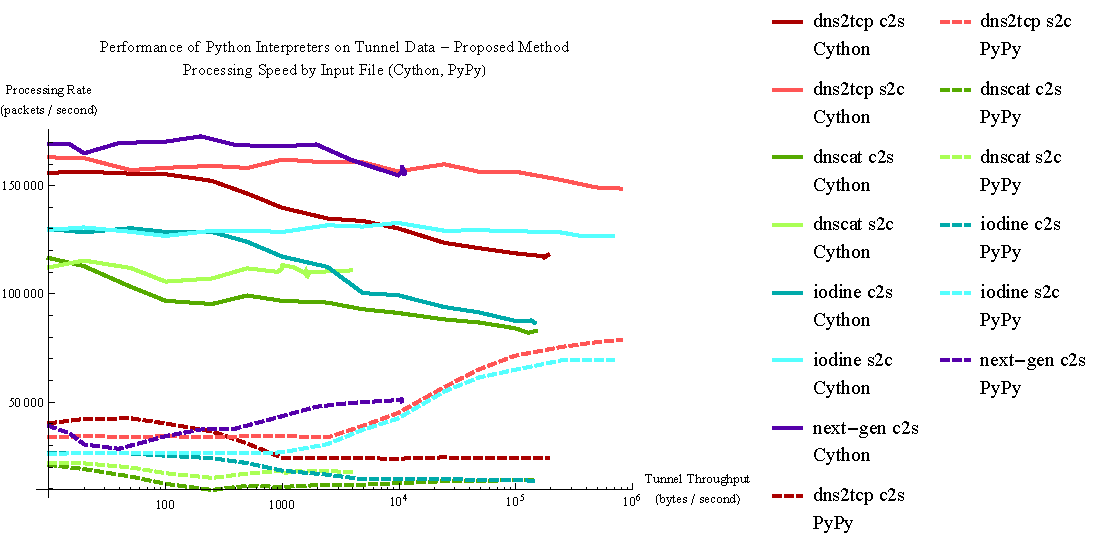
\includegraphics[width=\textwidth]{figures/ppia-proposed.pdf}
\caption[Performance of the Proposed Method on Tunnel Data by Python
Interpreter]{Performance of the proposed method on separated tunnelling
application data, showing processing rate as a function of input rate.}
\label{ppia-proposed}
\end{figure}

The proposed approach shows performance characteristics and trends that match
the naive approach far more closely than either of the other two approaches.
There is minimal degradation in performance for most of the tunnelling
applications, and almost all of the samples under the Cython interpreter are
above one hundred thousand packets per second. It is noteworthy that only
DNS2TCP's server-to-client remained above that threshold for throughputs beyond
five kilobytes per second for Paxson's approach. For Born's approach, only
DNS2TCP and Iodine's server-to-client transfers and the next-gen tunnel remained
above that threshold for throughputs above five kilobytes per second.

It is instructive to observe that PyPy's performance overall is considerably
lower than Cython on tunnel data, but as is show in figure \ref{pmqr}, this is
not the case on real-world data. The reasons for this may involve intricacies of
the dataset used, the JIT components of PyPy, and the effects of large amounts
of data on Cython's internal structures in this workload. PyPy is a viable
choice for some of the methods on real-world data despite being considerably
less optimal than Cython in all cases when working with tunnel application data.

\subsection{Processing Performance Conclusion}
As has been shown, the detection methods were tested on both real world and
purpose-generated tunnel application traffic as well as on two different Python
interpreters and were instrumented for their processing performance.

In the real world data test, the Cython interpreter performed well with the PyPy
interpreter matching or exceeding its performance for Born's and the proposed
detection methods. When operating on tunnelling application data, the Cython
interpreter is categorically faster in every case than PyPy with performance
factors ranging from two to two hundred depending on the application,
throughput, and method.

When evaluating the detection methods performance on real-world data, in all
cases the naive method is the fastest, followed by the proposed approach, Born's
method, and Paxson's method in order. Under the Cython interpreter, the naive
method is approximately fifty percent faster than the proposed method. The
proposed method is approximately twenty five to thirty percent faster than Born
and Paxson's approaches respectively. Under the PyPy interpreter, however, the
performance of the proposed method, and the naive method are very close with a
difference dropping to less than ten percent and Born's approach a close third
place. Paxson's method falls to the slowest position under the PyPy interpreter.

When operating on tunnelling application traffic, the average performance of the
methods (averaged over all tunnels and cases) can be seen in figure \ref{pmat} where
the naive and proposed methods both perform well, maintaining processing rates
in excess of one hundred twenty thousands packets per second. Born and Paxson's
approaches both suffer severe degradation of performance as throughput
increases, resulting in final processing rates well below one hundred thousand
packets per second. As was mentioned above, when looking at the tunnelling
applications individually (and not as an aggregate), only the naive and proposed
approaches are able to maintain processing rates above one hundred thousand for
all (or most, in the case of the proposed approach) of the tunnelling
applications and throughputs. Additionally, only the naive and proposed
approaches a re able to prevent significant performance degradation, and in fact
show very similar trends when their plots are compared directly.

\begin{figure}
\centering
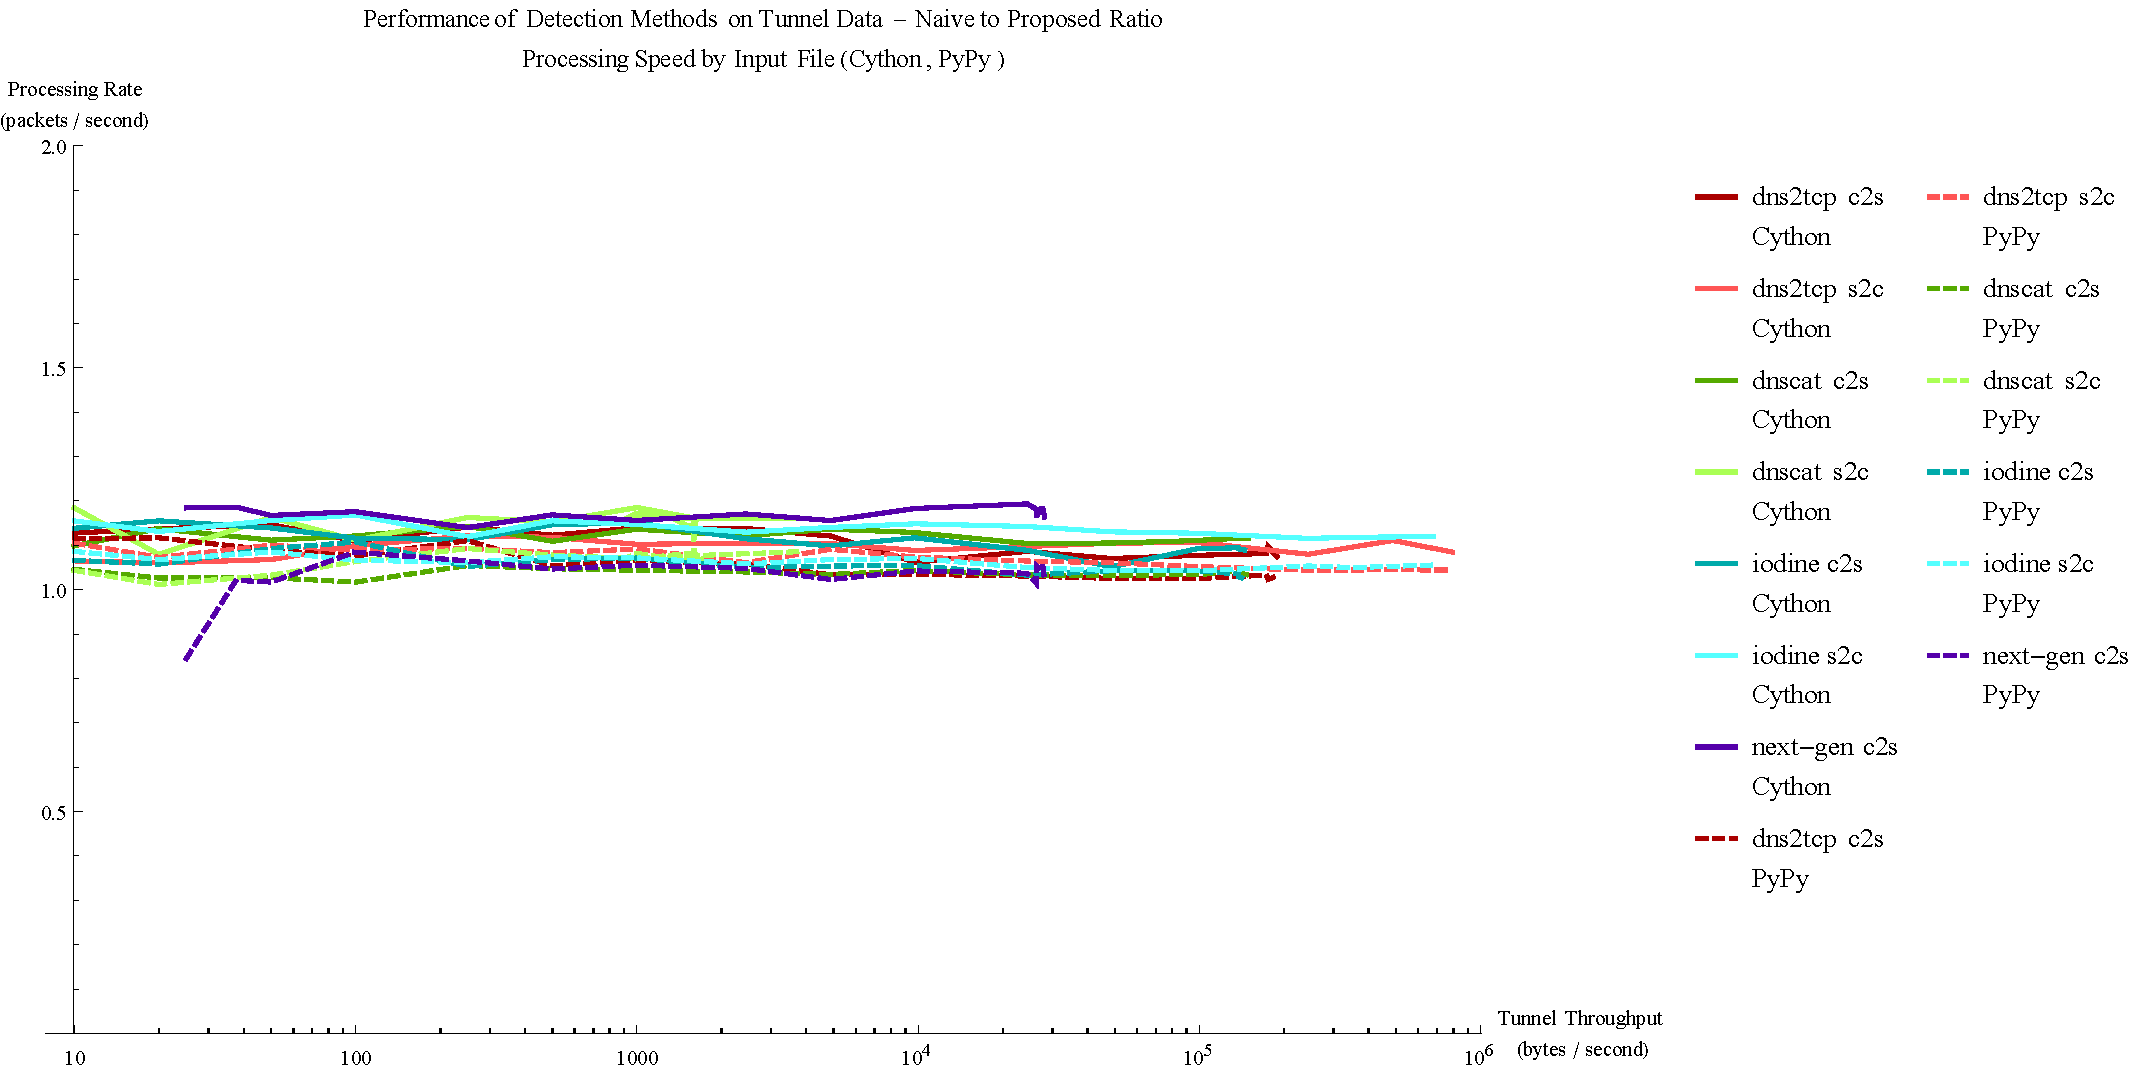
\includegraphics[width=\textwidth]{figures/ppia-naive2proposed.pdf}
\caption[Performance Ratio of the Naive Method to the Proposed Method on Tunnel
Data by Python Interpreter]{The ratio of the performance of the naive method to
the proposed method on separated tunnelling application data, with the vertical
axis showing the speedup of the naive method over the proposed method.}
\label{ppia-naive2proposed}
\end{figure}

When the ratio of the performance of the naive method to the proposed method, a
clustering very close to a fixed value is observed as in figure
\ref{ppia-naive2proposed}. This indicates that much of the performance
degradation, and potentially other performance characteristics, of the two methods
are dominated by the common scaffolding and/or the Python interpreter as opposed to by the underlying methods or
their implementation.

Through this examination, it has been shown that the proposed method
out-performs both methods from the literature by a considerable margin and comes
very close to matching the naive method in performance in many cases. This by
itself demonstrates a useful contribution of the proposed method, provided that
it is able to detect the tunnelled applications with a sufficiently high
certainty.

\chapter{Tunnel Detection Evaluation}
\label{chap-evaluation}
%\section{Baseline}
%\section{Tunnel Data}
%\subsection{Iodine}
%\subsection{dnscat}
%\subsection{DNS2TCP}
%\subsection{Nextgen}
%\section{Packet Throughput Performance}
%\section{Tunnel Detection Performance}
\label{tunnel-detection-performance}

The processing performance of the detection methods was examined in the previous
chapter which demonstrated that the proposed method is able to process packets
at a considerably higher rate than Born and Paxson's methods. This section will
compare the ability of the methods to detect tunnelled application data and
compare the detection results of the methods against each other.

Figure \ref{mbtt} shows several log-log plots (in order to be able to have
adequate resolution for both very small and very large throughputs), one for
each detection method, that demonstrates how the metrics generated by the
methods scale as the throughput of the tunnel is increased. The expected trends
of the detection methods is as follows:

\begin{itemize}
\item The naive metric is expected to increase with throughput with a slope
dependant on the implementation. In practice, all of the implementations have a
slope of approximately one.

\item Born's metric is expected to decrease to zero for tunnels as their
character distribution approaches uniform. This is the behaviour seen for most
tunnels with the exception of the Iodine and DNS2TCP server-to-client transfers
as well as the next-gen tunnel. The next-gen tunnel's behaviour is precisely as
expected due to its construction specifically to evade character frequency
analysis such as is used in Born's approach.

\item Paxson's metric is expected to increase approximately linearly with a
slope that depends on the implementation and on the compressibility of the
transferred data. Because the transferred data is pseudorandom, it is nearly
incompressible and thus the observed slops of the lines is derived from the
implementation details of the various tunnelling applications.

\item The proposed metric is expected to increase approximately logarithmically
with additional throughput due to its reliance on entropy as a multiplicative factor in its final metric. This is the
behaviour seen for all except for Iodine's server-to-client transfer, with
varying scaling factors.
\end{itemize}

As is visible in figure \ref{mbtt}, tunnels with lower throughput produce
categorically smaller metrics, making them more difficult to detect,
as will be seen later in figures \ref{mpnv}, \ref{mpbv}, \ref{mppv}, and
\ref{mphv}. Because of this, the methods will be tested on their ability to
detect the most hidden tunnel of each application, which in practice is the
tunnel that transmits only ten bytes per second, against background normal DNS
traffic. The assumption, which proves true in practice, is that tunnels that
move more data are necessarily easier to detect, and the most dangerous tunnels
are those that go undetected. By testing the methods to ensure they detect
low-rate tunnels, their ability to detect high-rate tunnels is implicitly
demonstrated.

The network traffic, both real-world and the tunnelling application traffic, was
bucketed into ten-second wide windows for processing. This window size is much
smaller than may be commonly used, but was chosen in order to present the most
pessimistic environment possible to the detection methods in order to be able to
discern their capabilities.

\begin{landscape}
\begin{figure}
\centering
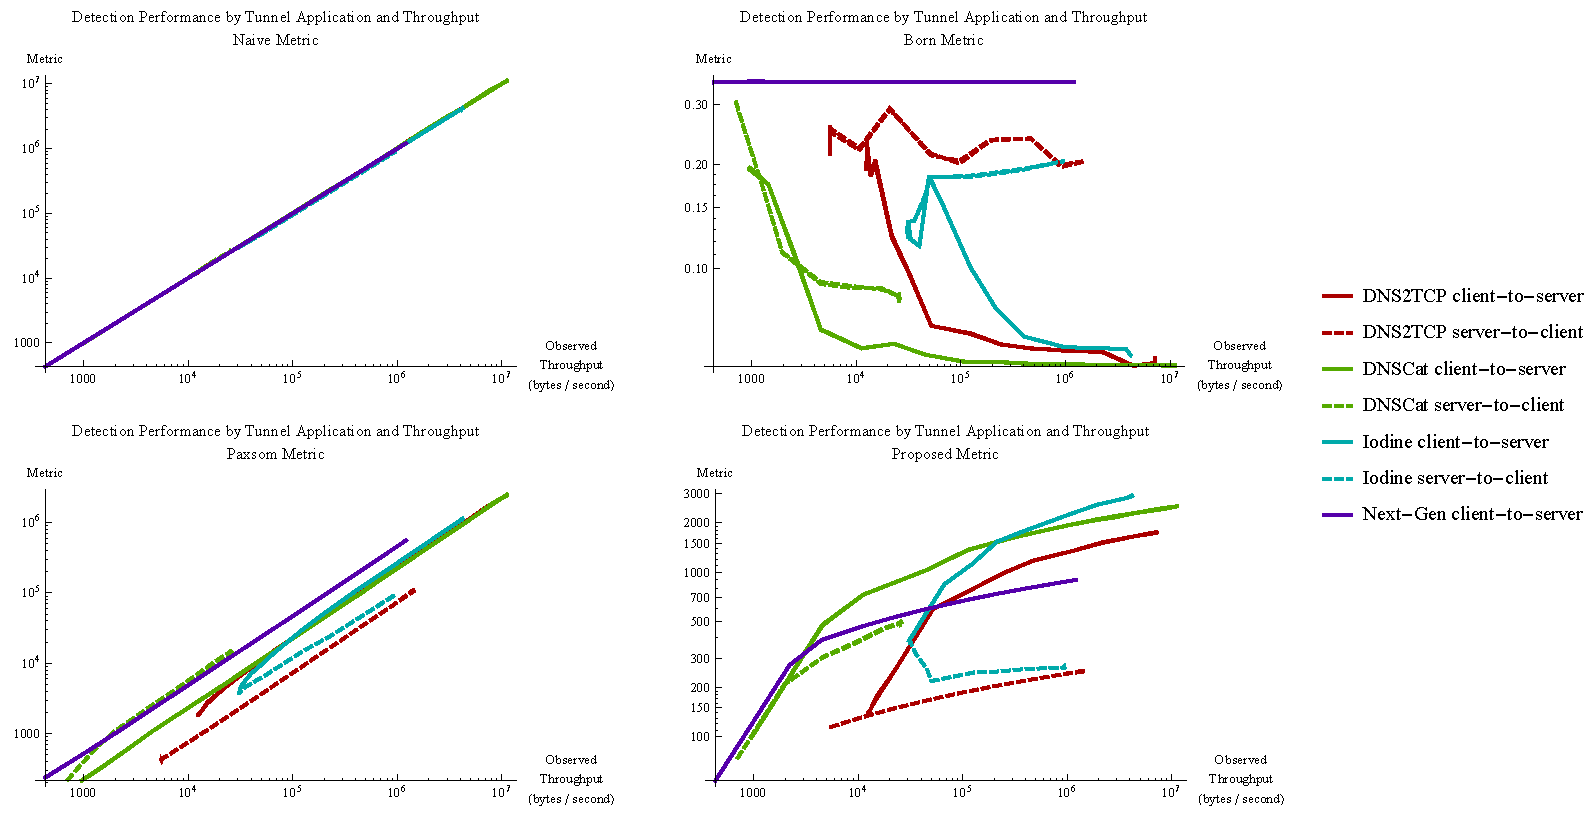
\includegraphics[width=1.4\textwidth]{figures/mpbtt.pdf}
\caption[Scaling of Detection Metrics by Tunnel Throughput]{These plots show how
the metrics computed by the various detection methods scale per tunnelling
application as a function of the tunnel throughput rates. Note that since not
all tunnels are capable of a full range of throughputs (some generate a minimum
amount of traffic, regardless of how low the throughput is), resulting in some
of the shorter plots.}
\label{mbtt}
\end{figure}
\end{landscape}

\section{Detection Performance Against Real World Data}
\label{detection-perf}

The plots shown here illustrate how the various tunnel application fare when
compared to normal traffic. On each plot the vertical axis is "percent of
samples with a metric greater than $x$" with the horizontal axis being the
metric produced by the method. The black curve represents normal traffic, with
the vertical coloured bars representing the various DNS tunnels. The vertical bars,
coloured and dashed/solid according to the legend, mark the target throughput
levels given in section \ref{tunapptp}, but are not identified otherwise. As can
be seen in figure \ref{mbtt}, in almost all cases (with any exceptions occurring for higher throughputs), the metric is approximately
monotonic with the lowest throughput samples having the smallest metric. Due to
the plot ranges on the following figures, not all bars are visible on all plots.
Due to the tendency of Born's metric to produce small values for tunnels, most
of the tunnel bars are visible on the plot of Born's metric.

Due to the layout of the plots, the approximate detectability of a tunnel is
related to the $y$ value of the crossing of the vertical markers with the normal
curve. This crossing indicates how near the outliers the marker sits with an
intersection at $y$ values very near 0 or 1 representing the best detection
probability. The closer to the outliers the tunnel is measured to be, the less
ambiguity there is as to whether or not the analyzed traffic represents normal
traffic or not. A value of 0 or 1 would indicate a perfectly detectable tunnel,
while a value of 0.5 would indicate a tunnel that suffers from a very high
ambiguity of classification. This value will be referred to as the
\emph{crossing value} in subsequent discussion.

\begin{figure}
\centering
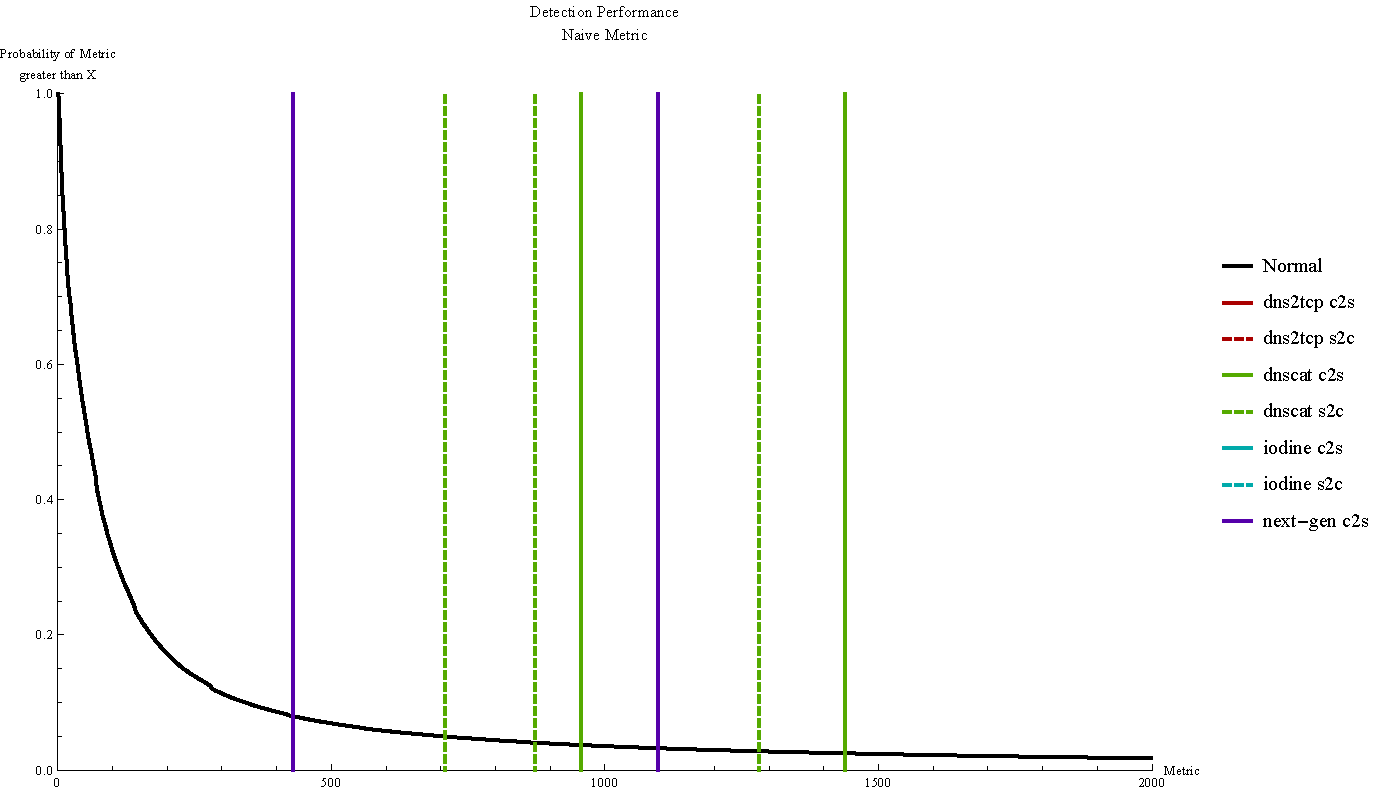
\includegraphics[width=\textwidth]{figures/mpnv.pdf}
\caption[Tunnel Detection Performance - Naive Metric]{This visualizes the
ability of the naive metric to discern a DNS tunnel from normal DNS traffic.}
\label{mpnv}
\end{figure}

\begin{figure}
\centering
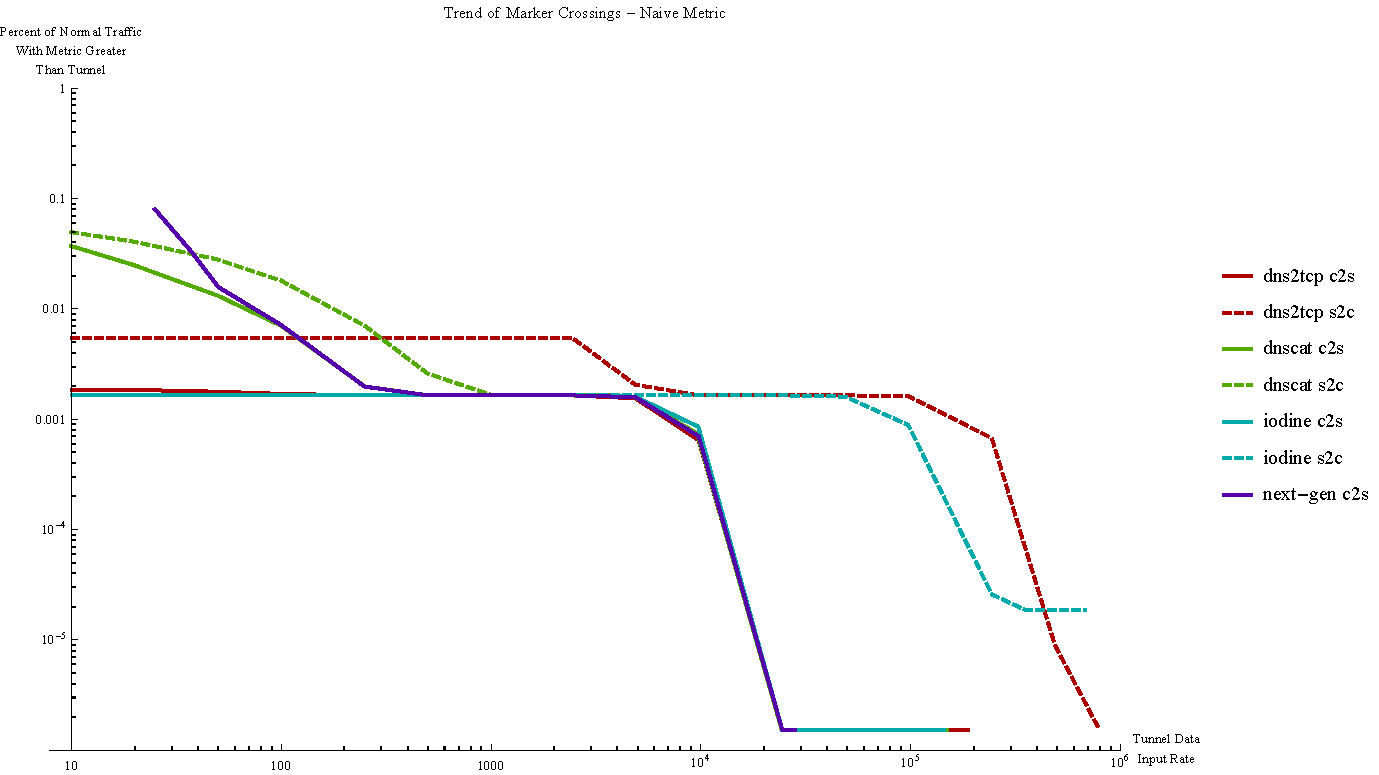
\includegraphics[width=\textwidth]{figures/cnplot.pdf}
\caption[Trend of Crossing Value for Tunnels - Naive Metric]{This plot shows the
trend of the crossing values for tunnels when compared to real-world data for the
naive metric.}
\label{cnplot}
\end{figure}

Figure \ref{mpnv} shows the performance of the naive metric, with markers
visible for the next-gen and DNSCat tunnels. The lowest marker belongs to the
next-gen tunnel, and crosses at a value of 0.0799815, followed by a DNSCat
server-to-client transfer crossing at 0.0496253. Iodine's client-to-server
transfers are the most easily detectable with its lowest transfer rate crossing
at 0.00164529 indicating a very low ambiguity when classifying its traffic.

The naive method, due to the nature of the the capture involving very few
duplicate queries, performs quite well overall even on the next-gen tunnel
traffic. Figure \ref{cnplot} shows the trends of the crossing values for the
tunnelling applications as a function of the data throughput. This property
and its impacts were discussed in section \ref{implementation-naive} in greater
detail.

\begin{figure}
\centering
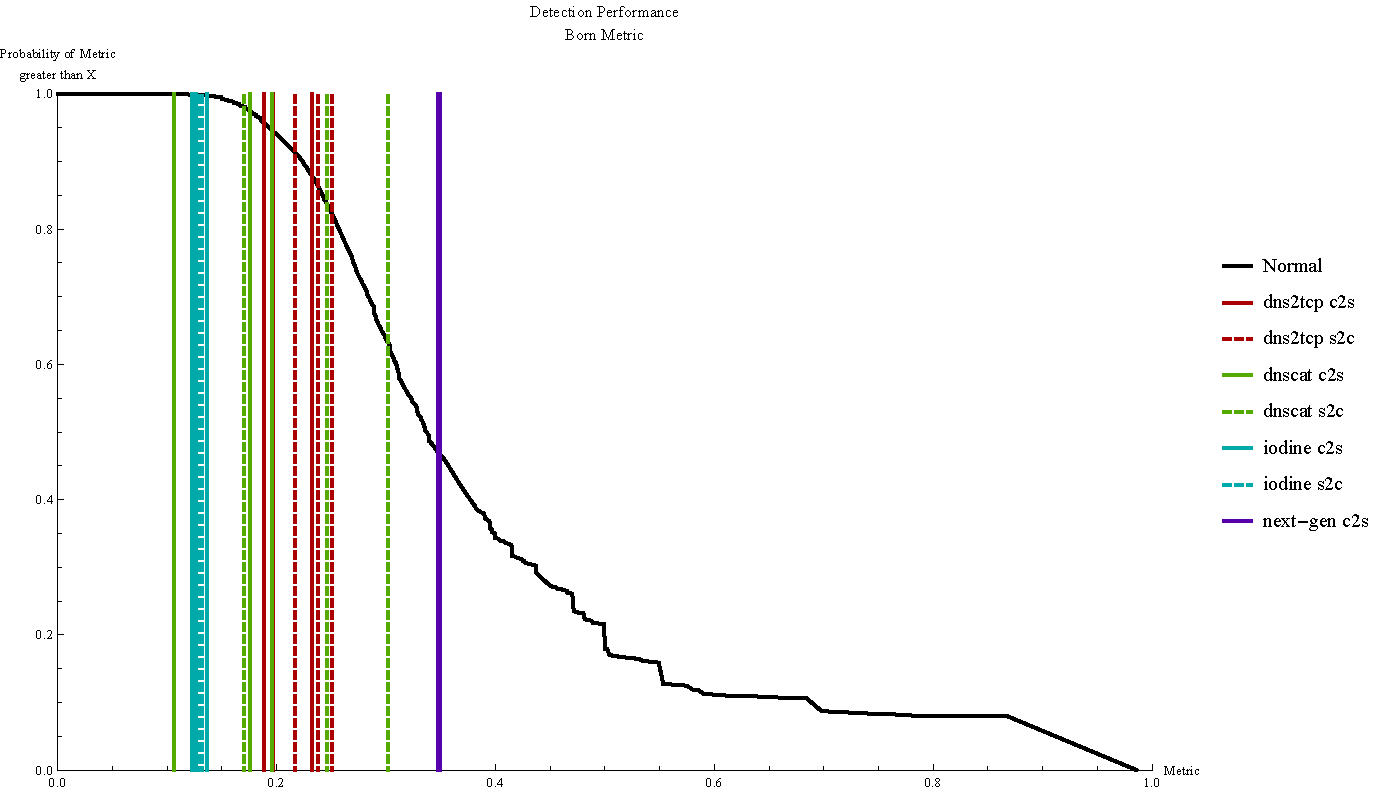
\includegraphics[width=\textwidth]{figures/mpbv.pdf}
\caption[Tunnel Detection Performance - Born's Metric]{This visualizes the
ability of Born's metric to discern a DNS tunnel from normal DNS traffic.}
\label{mpbv}
\end{figure}

\begin{figure}
\centering
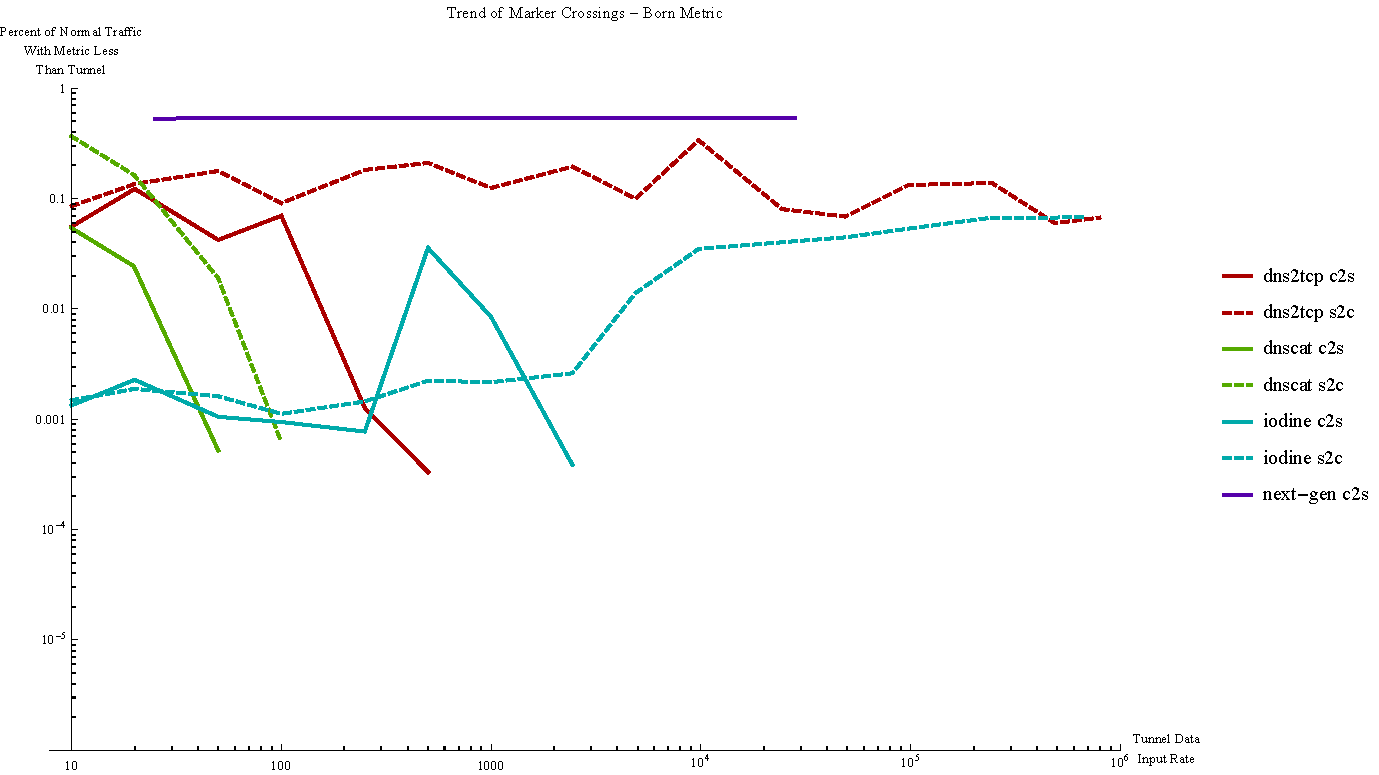
\includegraphics[width=\textwidth]{figures/cbplot.pdf}
\caption[Trend of Crossing Value for Tunnels - Born's Metric]{This plot shows
the trend of the crossing values for tunnels when compared to real-world data 
for Born's metric.}
\label{cbplot}
\end{figure}

Figure \ref{mpbv} shows the performance of Born's metric with almost all markers
visible clustered near the smaller metric values. Since the implementation of
Born's metric produces smaller metrics for tunnels, the highest values are the
ones of interest. The highest crossing value of 0.529347 occurs for the next-gen
tunnels. It is not easily seen in the plot, but all sixteen of the next-gen
tunnel markers are superimposed on each other at that value. This is due to how
the tunnel was implemented for the proof-of-concept, as all traffic generated
very closely conforms to a specified distribution. This distribution produces a
particular metric under the implementation of Born's approach, independent of
the amount of throughput. The next-gen tunnel markers are followed by the DNSCat
server-to-client marker with a crossing value of 0.367036. Similarly to the
naive metric, Iodine's client-to-server tunnel was the most easily detected
tunnel with the lowest throughput samples achieve a crossing value of
0.00133572.

It is easily seen that Born's metric will not be able to identify the next-gen
tunnel with any reasonable certainty due to the ambiguity caused by the tunnel's
traffic generating metrics very near to the median of real-world traffic. It is
possible to augment the next-gen tunnel to adhere less tightly to a given
distribution in order to spread its metrics over a wider range surrounding the
median, further increasing the difficulty of detection. Figure \ref{cbplot}
shows the trends of the crossing values for the tunnelling applications as a
function of the data throughput.

%\begin{figure}
%\centering
%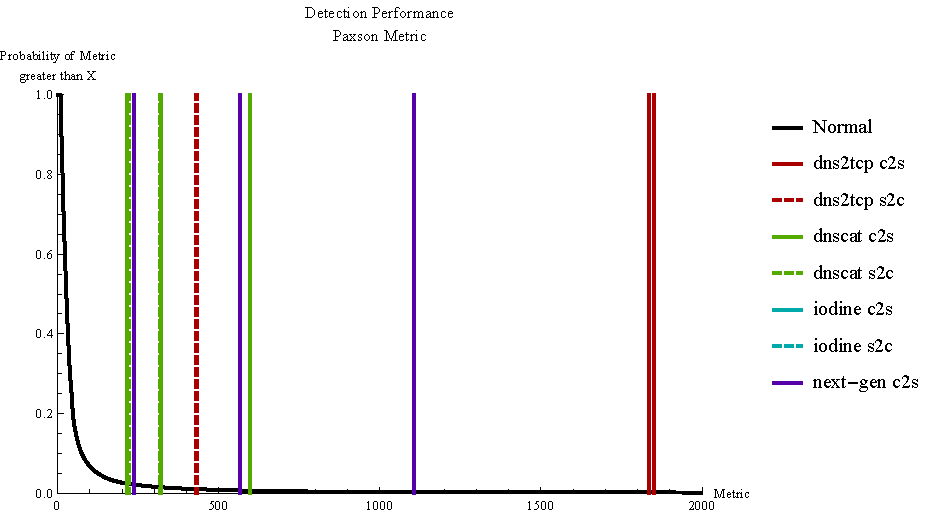
\includegraphics[width=\textwidth]{figures/mppv.pdf}
%\caption[Tunnel Detection Performance - Paxson's Metric]{This visualizes the
%ability of Paxson's metric to discern a DNS tunnel from normal DNS traffic.}
%\label{mppv}
%\end{figure}

\begin{figure}
\centering
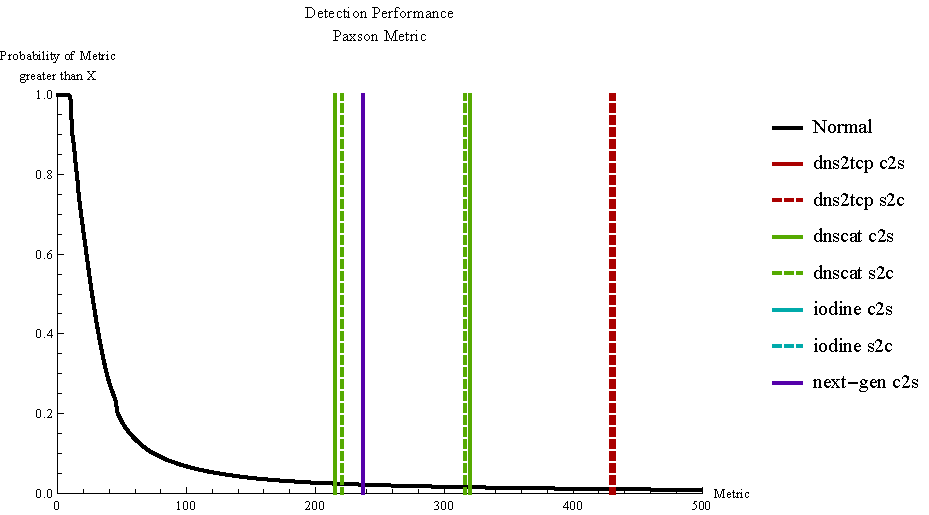
\includegraphics[width=\textwidth]{figures/mppv-500.pdf}
%\caption[Tunnel Detection Performance - Naive Metric (Truncated View)]{A cropped
%plot of figure \ref{mppv} that offers more resolution in the smaller metric
%ranges.}
%\label{mppv-500}
\caption[Tunnel Detection Performance - Paxson's Metric]{This visualizes the
ability of Paxson's metric to discern a DNS tunnel from normal DNS traffic.}
\label{mppv}
\end{figure}

\begin{figure}
\centering
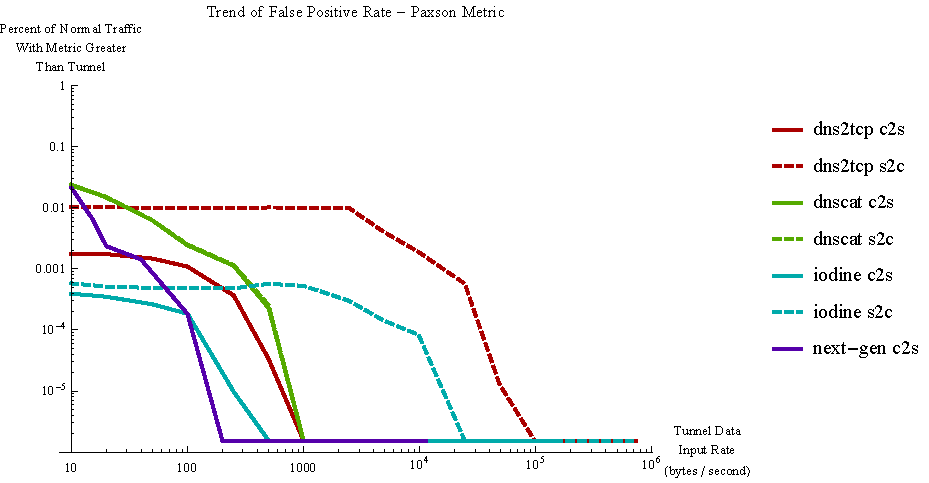
\includegraphics[width=\textwidth]{figures/cpplot.pdf}
\caption[Trend of Crossing Value for Tunnels - Paxson's Metric]{This plot shows
the trend of the crossing values for tunnels when compared to real-world data for
Paxson's metric.}
\label{cpplot}
\end{figure}

Figure \ref{mppv} shows the performance of Paxson's metric similar to the plot
shown for the naive method. The lowest metric is shown by the DNSCat
client-to-server transfer with crossing value of 0.0239753 followed very closely
by DNSCat's server-to-client transfer with a crossing value of 0.0239753. The
next-gen tunnel produces a crossing value of 0.0212873 and again Iodine is the
most easily detected with its client-to-server transfers producing crossing
values no larger than 0.00392552.

As is expected, Paxson's method shows considerable improvement over both the
approach proposed by Born and the naive method in terms of ambiguity of tunnel
detection. Figure \ref{cpplot} shows the trends of the crossing values for the
tunnelling applications as a function of the data throughput.

%\begin{figure}
%\centering
%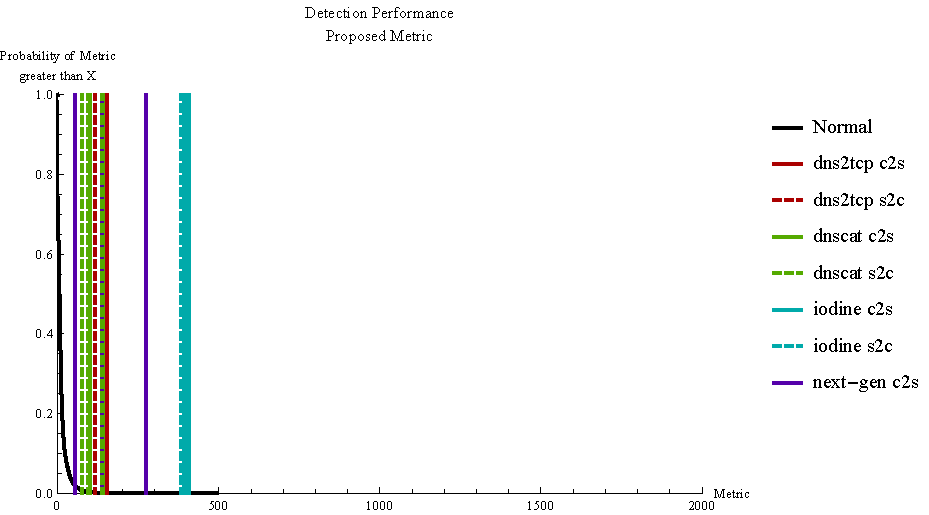
\includegraphics[width=\textwidth]{figures/mphv.pdf}
%\caption[Tunnel Detection Performance - Proposed Metric]{This visualizes the
%ability of the proposed metric to discern a DNS tunnel from normal DNS traffic.}
%\label{mphv}
%\end{figure}
\begin{figure}
\centering
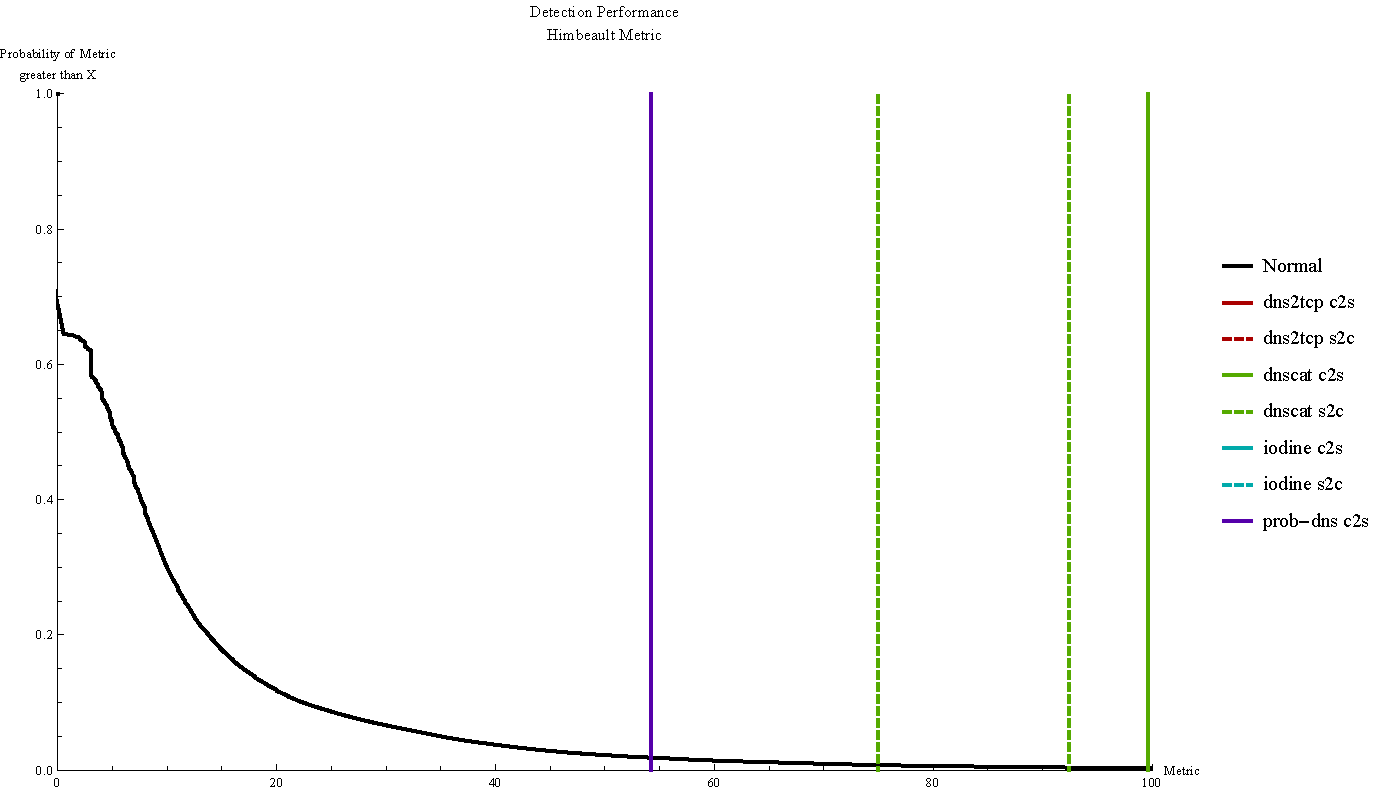
\includegraphics[width=\textwidth]{figures/mphv-100.pdf}
%\caption[Tunnel Detection Performance - Proposed Metric (Truncated View)]{A
%cropped plot of figure \ref{mphv} that offers more resolution in the smaller
%metric ranges.}
%\label{mphv-100}
\caption[Tunnel Detection Performance - Proposed Metric]{This visualizes the
ability of the proposed metric to discern a DNS tunnel from normal DNS traffic.}
\label{mphv}
\end{figure}

\begin{figure}
\centering
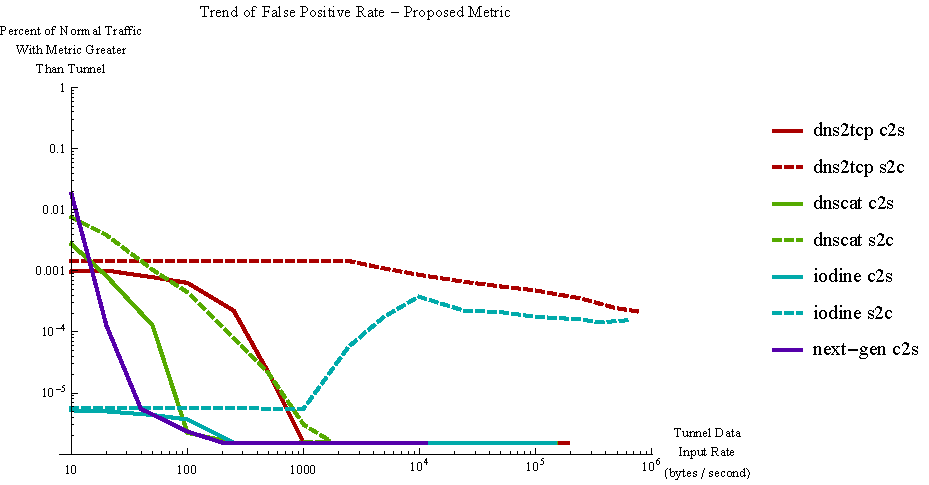
\includegraphics[width=\textwidth]{figures/chplot.pdf}
\caption[Trend of Crossing Value for Tunnels - Proposed Metric]{This plot shows
the trend of the crossing values for tunnels when compared to real-world data for
the proposed metric.}
\label{chplot}
\end{figure}

Figure \ref{mphv} shows the performance of the proposed metric in a fashion
similar to the naive method and for Paxson's method. The first crossing value
encountered is from the next-gen tunnel at 0.0184927. This is followed by two of
the samples generated by the DNSCat server-to-client transfers, the first of
crossing value being at 0.00751152. As has been the case for all metrics thus
far, Iodine is the most easily detected tunnel generating crossing values for
its lowest throughput client-to-server and server-to-client of
$5.19129\times10^{-6}$ and $5.73392\times10^{-6}$ respectively.

The proposed approach produces the lowest crossing values of all approaches,
with the figure \ref{chplot} showing the trends of the crossing values for the
tunnelling applications as a function of the data throughput.

\section{Certainty and Ambiguity of Tunnel Classification}
\label{detection-perf-cert}

It is possible to simplify the above plots and figures into a single chart that
plots the minimum detection certainty observed for each method and each
tunnelling application. The certainty shown in the following plots is
intuitively a measure of how much ambiguity there is when classifying the tunnel
sample based on how far the sample lies from 'typical' normal traffic. It is
calculated as

\[\textrm{certainty}=1-\textrm{crossing\_value}\]

The following charts only consider the certainty of detecting the tunnel in
which the method is least certain. By comparing the methods in their most
hostile scenarios more substantial distinctions can be observed with clearer
separation between the best two methods. In all cases, this corresponded to one
of the tunnelling applications at the ten bytes per second throughput level,
which demonstrates the effectiveness of these methods to solve the
\emph{needle-in-a-haystack} problem of low throughput DNS tunnels on a very busy
network link.

\begin{figure}
\centering
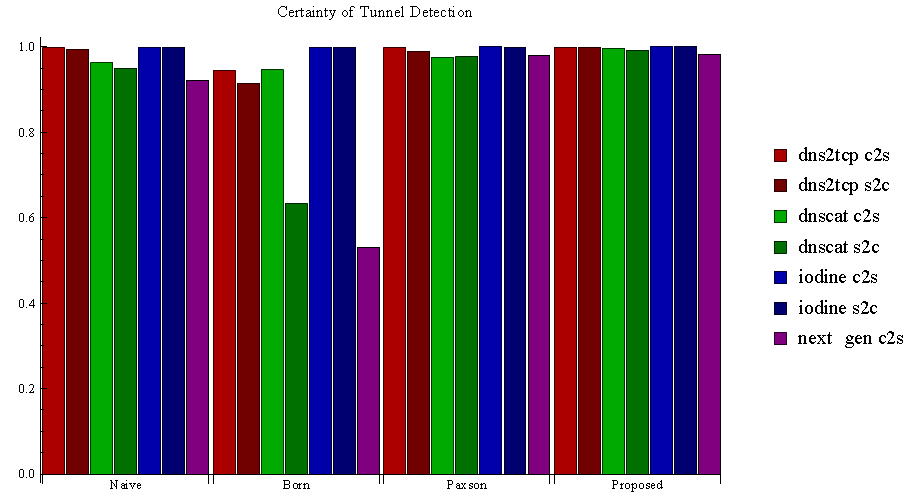
\includegraphics[width=\textwidth]{figures/cplot.pdf}
\caption[Chart of Certainty of Detection by Tunnel Application and Detection
Method]{Comparison of the certainty of classification of a tunnel against
real-world traffic for the least certain tunnel in each detection scenario
(method/application pair).}
\label{cplot}
\end{figure}

Figure \ref{cplot} shows the certainties of each method for each tunnelling
application, with the certainty in the interval $[0,1]$. Observe the extremely
low certainty of Born's metric on two tunnelling applications (next-gen and
DNSCat's server-to-client), with lackluster performances for DNSCat's
client-to-server and both DNS2TCP transfer directions. The only tunnelling
application that Born's method reliably picks out is Iodine, however as was
shown earlier Iodine was by far the most easily distinguished tunnel by a large
margin for all detection methods. The naive and proposed methods as well as
Paxson's method perform similarly with differences that are not easily
distinguished in this chart.

\begin{figure}
\centering
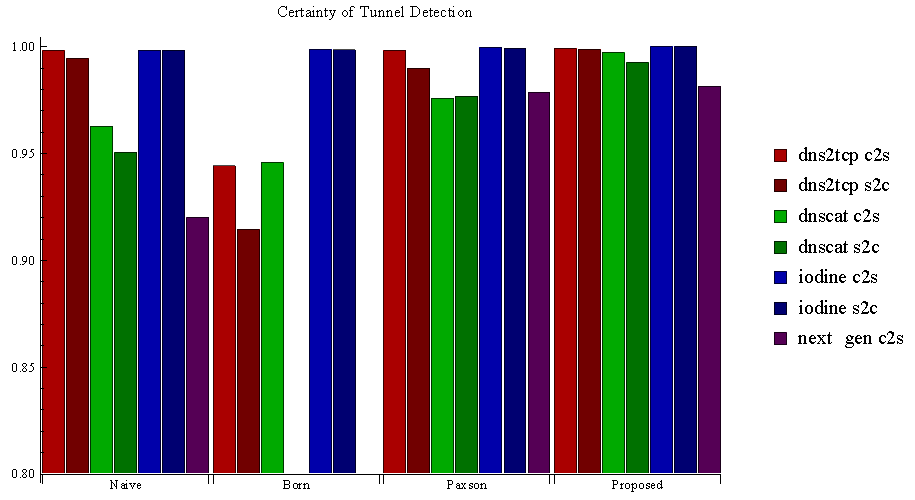
\includegraphics[width=\textwidth]{figures/cplot2.pdf}
\caption[Chart of Certainty of Detection by Tunnel Application and Detection
Method - 0.80 to 1.00]{Figure \ref{cplot} replotted with a reduced range to
accentuate small differences.}
\label{cplot80}
\end{figure}

Figure \ref{cplot80} shows the same data as in figure \ref{cplot} with a
restricted range spanning the interval $[0.80,1.00]$ as opposed to $[0,1]$. This
restricted charting range makes the the differences between the top performing
methods more easily visible. In this chart, it is easily seen that the naive
method outperforms Born's method in all except the Iodine case. The Iodine
performance differences are not easily visible due to the very close values. The
naive method has a certainty of 0.998355 for both transfer directions while
Born's method has certainties of 0.998664 and 0.998512 for the client-to-server
and server-to-client directions respectively. The differences, on the order of
0.0003, are not visible in the charts. The performance of the proposed method
and Paxson's method relative to the naive method is clearly visible in this
chart.

\begin{figure}
\centering
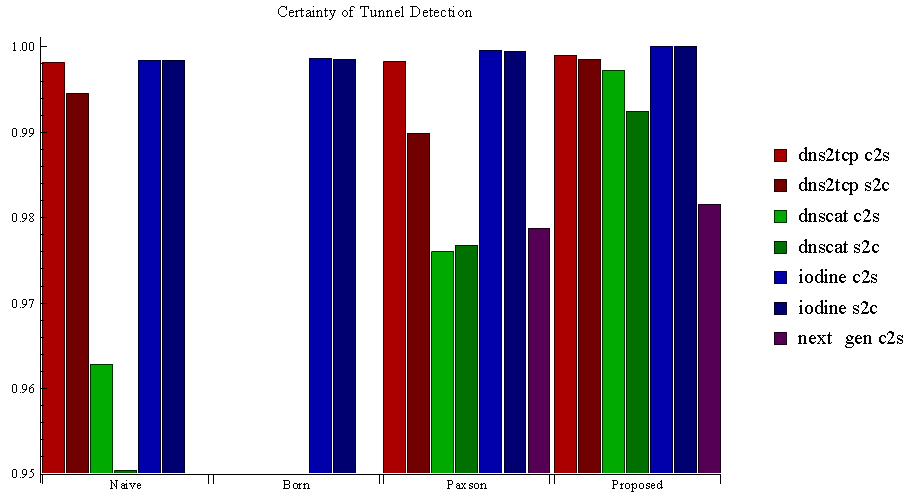
\includegraphics[width=\textwidth]{figures/cplot3.pdf}
\caption[Chart of Certainty of Detection by Tunnel Application and Detection
Method - 0.95 to 1.00]{Figure \ref{cplot} replotted with a reduced range to
accentuate \emph{very} small differences.}
\label{cplot95}
\end{figure}

The differences between Paxson's method and the proposed method are visible, but
an additional chart further accentuating them is instructive and is shown in
figure \ref{cplot95}. In this final chart which shows a range of certainties in
the interval $[0.95,1.00]$, the differences between the two methods are clearly
visible, with the proposed approach achieving a higher certainty in every
detection scenario.

\section{Tunnel Detection Performance Conclusion}
It is visible from the detailed plots in sections \ref{detection-perf} and
\ref{detection-perf-cert} that the proposed method is superior to its peers in
its ability to detect tunnels with certainty in excess of ninety eight percent.
This extremely high detection rate is achieved at a very short time scale and
with very low tunnel throughput. Depending on the tunnelling application,
detection performance rises above ninety nine percent for all except the
next-gen application, and above 99.999\% for Iodine.

\chapter{Conclusion}

In this work, a new method of detecting DNS tunnels was proposed, described, and
evaluated.

The existing landscape of detection methods was summarized (section
\ref{litreview}) and a gap identified indicating a need for a new method
(section \ref{methodreqs}) that has both high processing performance on
commodity hardware, and robust tunnel detection. A prototypical next-gen tunnel
application was postulated (section \ref{supertunnel}) and simulated in order to
present a more difficult detection task during evaluation alongside existing
detection methods. Several detection methods from the literature as well as the
proposed method were selected (section \ref{chosen-methods}) and implemented on
a common framework (section \ref{implementations}). The implemented methods were
tested for processing performance (section \ref{processing-perf}) and tunnel
detection performance on a large sample of real world DNS traffic as well as
existing and next-gen tunnelling application data (section
\ref{chap-evaluation}).

As is shown in the relevant sections, the proposed method outperforms its peers
in both processing performance and tunnel detection in almost every situation.
The exception is the naive method which outperforms the proposed method in
processing performance by approximately fifty percent at the expense of
detection performance. As was mentioned in section \ref{implementation-naive}
however, the naive method's detection performance is only as good as it is in
this case due to the lack of duplication of DNS queries.

The end product of these results is a contribution to the field comprising a new
detection method with superior processing and detection performance. The new
detection method falls short of matching the naive method's processing
performance in many situations with the trade off of far superior detection
performance.

\section{Future Work}

The proposed method was shown to highly effective in detecting the targeted network traffic with high performance, outperforming existing methods in almost every scenario. In order for this to be of value, however, an adoption of this method into an existing commercial product or an implementation as a plugin for an existing commonly deployed security framework would be necessary.

Future work could include implementing the proposed method for Bro, Snort, Suricata or other existing intrusion detection systems in order to improve organizations ability to observe DNS tunnels in their network.

%\begin{figure}
%\centering
%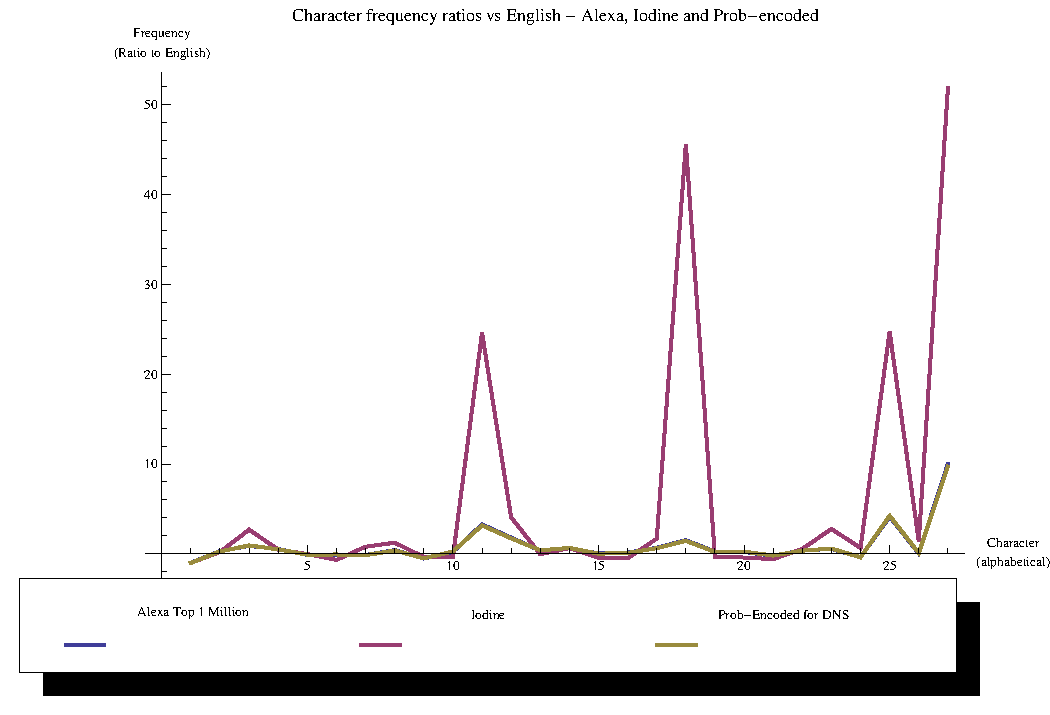
\includegraphics[width=4in]{figures/alexa_iodine_prob_v_english-r.pdf}
%\caption[DNS Query, Iodine and Prob-coded Comparison - Ratio]{A plot comparing the statistical properties of the Alexa top one million domains names, Iodine generated queries, and queries generated by the prob-coding tunnel software. This compares the frequencies of each charater in the three considered sets of output against the baseline of english.}
%\label{FIGURE_alexa-iodine-prob-v-english-r}
%\end{figure}
%
%\begin{figure}
%\centering
%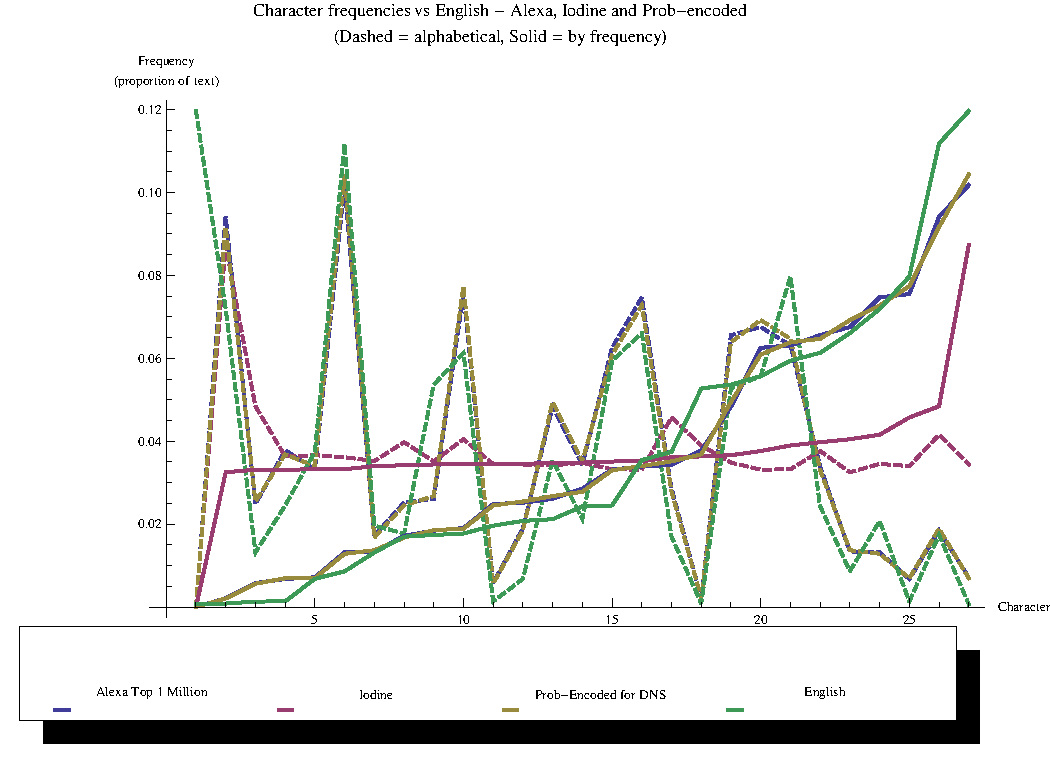
\includegraphics[width=4in]{figures/alexa_iodine_prob_v_english-a.pdf}
%\caption[DNS Query, Iodine and Prob-coded Comparison - Absolute]{A plot comparing the statistical properties of the Alexa top one million domains names, Iodine generated queries, and queries generated by the prob-coding tunnel software. This compares the absolute frequencies of each charater both sorted by character (dashed) and sorted by frequency (solid).}
%\label{FIGURE_alexa-iodine-prob-v-english-a}
%\end{figure}
%
%\begin{figure}
%\centering
%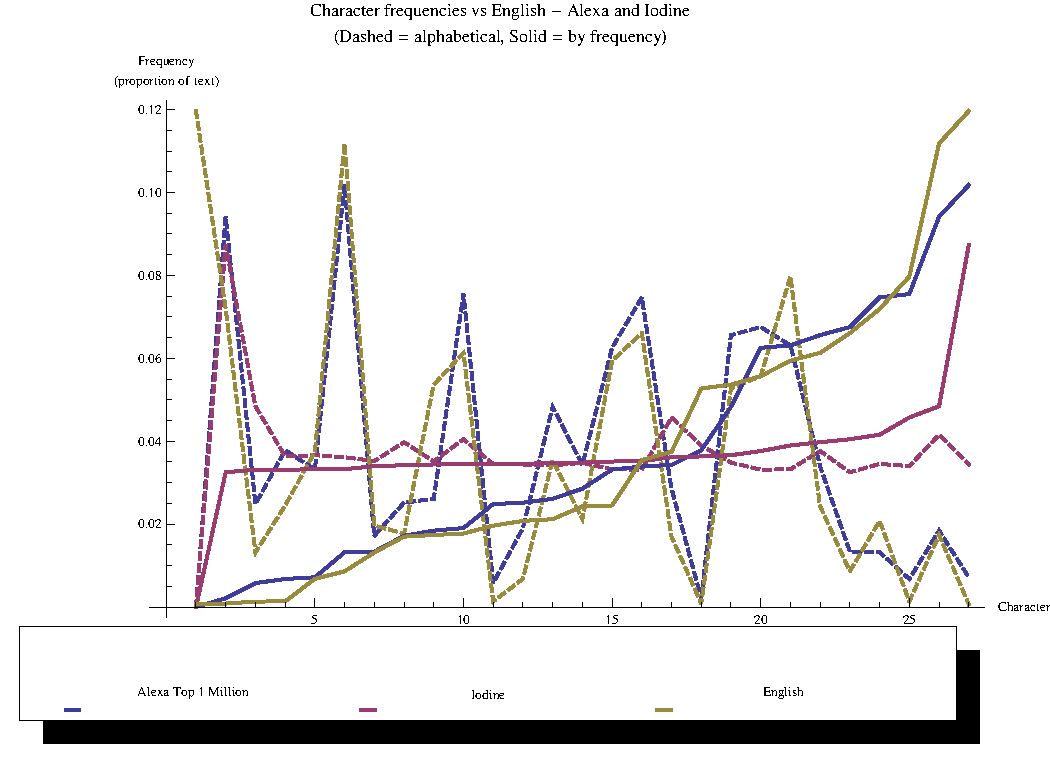
\includegraphics[width=4in]{figures/alexa_iodine_v_english-a.pdf}
%\end{figure}
%\begin{figure}
%\centering
%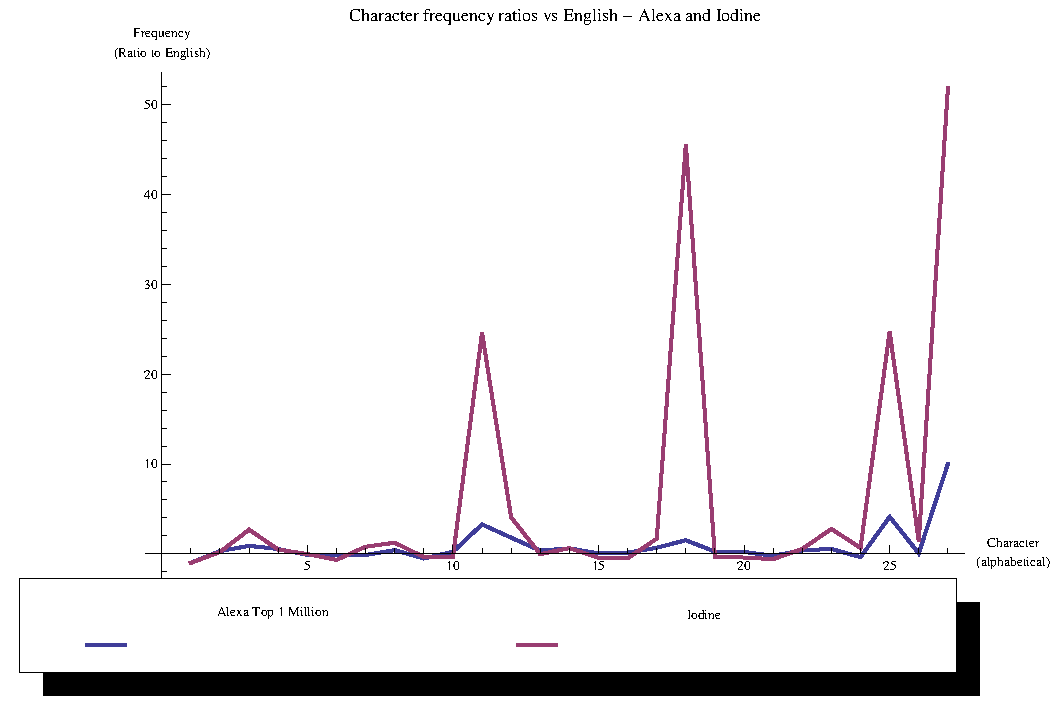
\includegraphics[width=4in]{figures/alexa_iodine_v_english-r.pdf}
%\end{figure}
%\begin{figure}
%\centering
%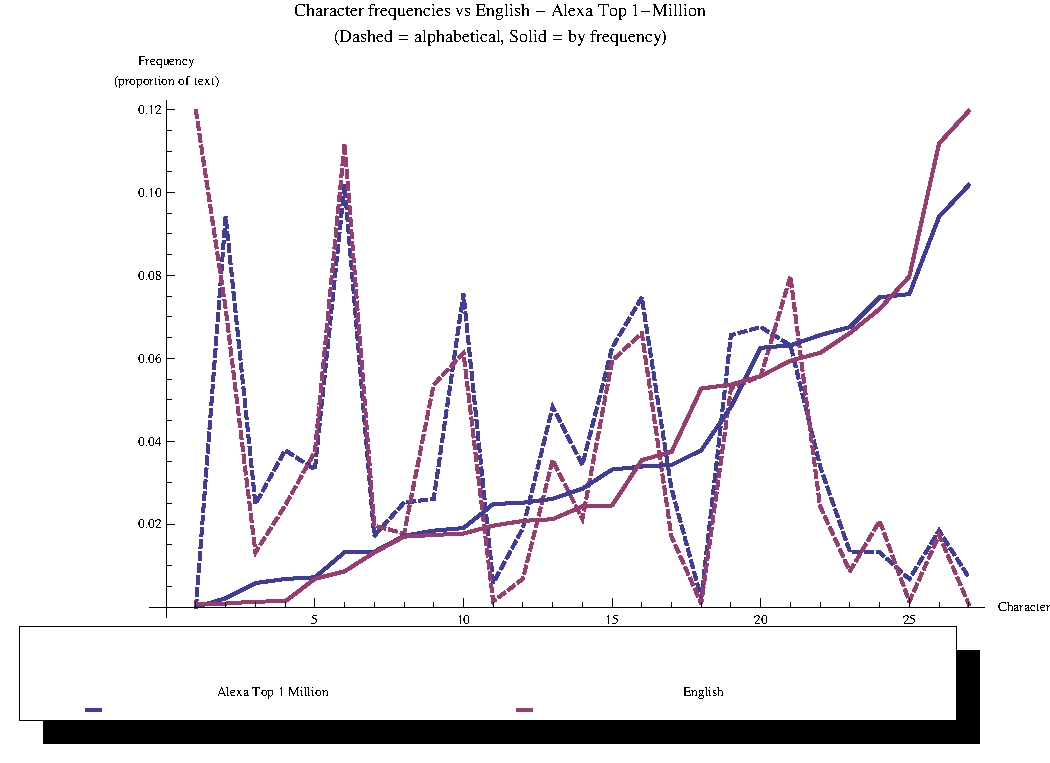
\includegraphics[width=4in]{figures/alexa_v_english-a.pdf}
%\end{figure}
%\begin{figure}
%\centering
%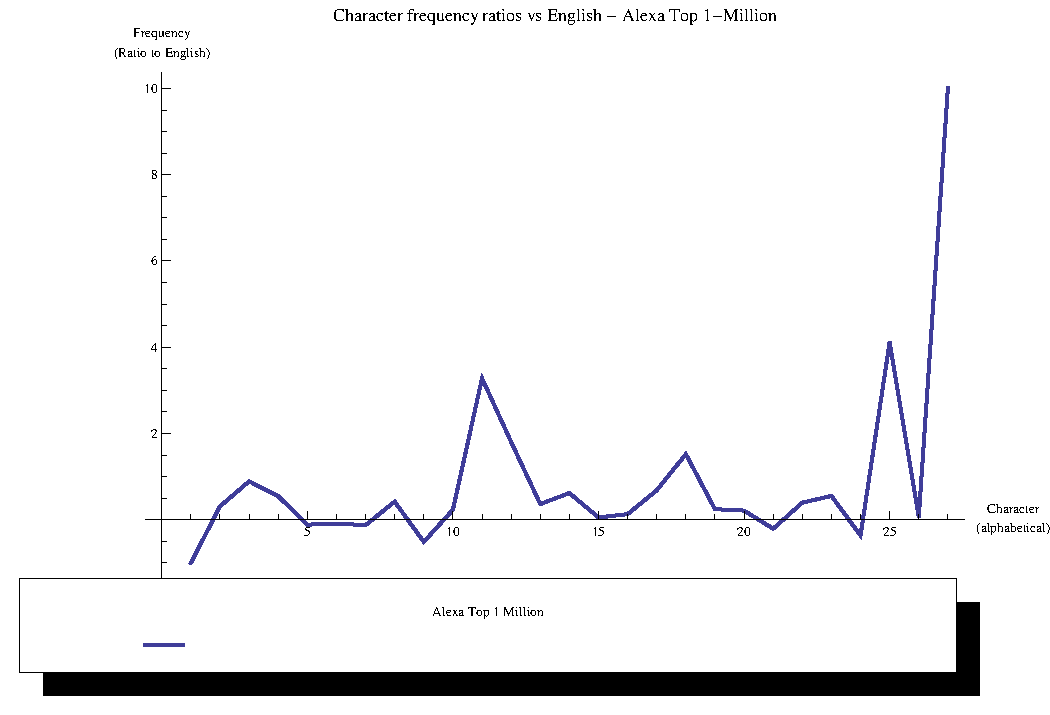
\includegraphics[width=4in]{figures/alexa_v_english-r.pdf}
%\end{figure}
%\begin{figure}
%\centering
%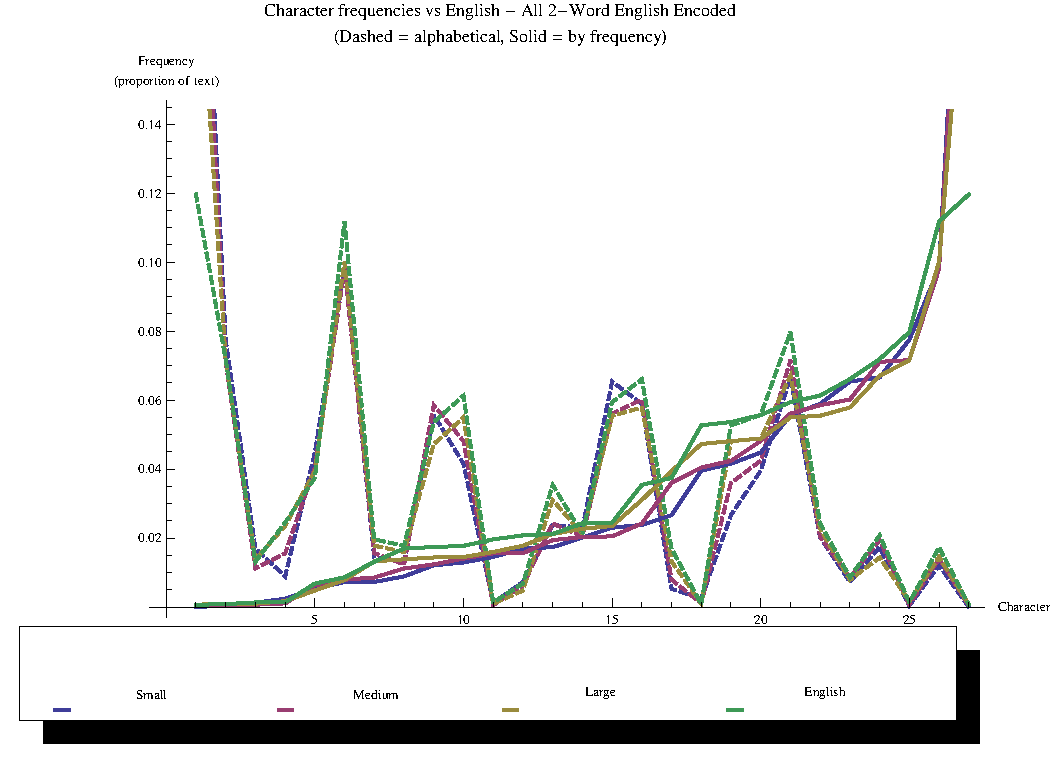
\includegraphics[width=4in]{figures/markov2-a.pdf}
%\end{figure}
%\begin{figure}
%\centering
%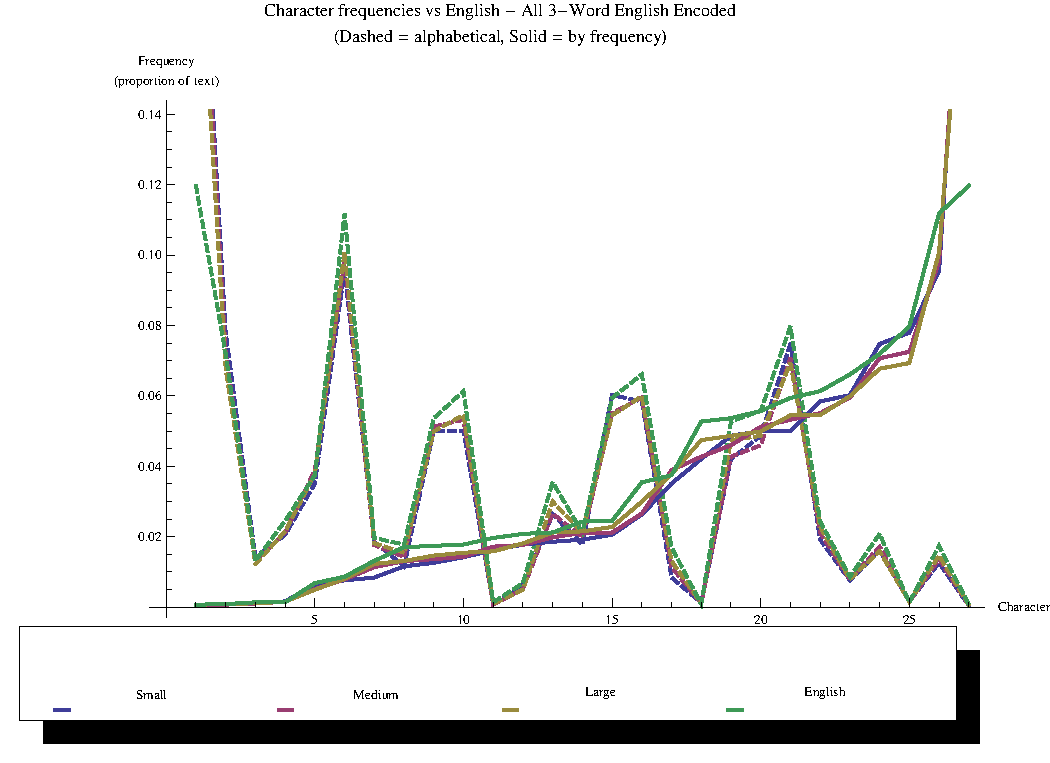
\includegraphics[width=4in]{figures/markov3-a.pdf}
%\end{figure}
%\begin{figure}
%\centering
%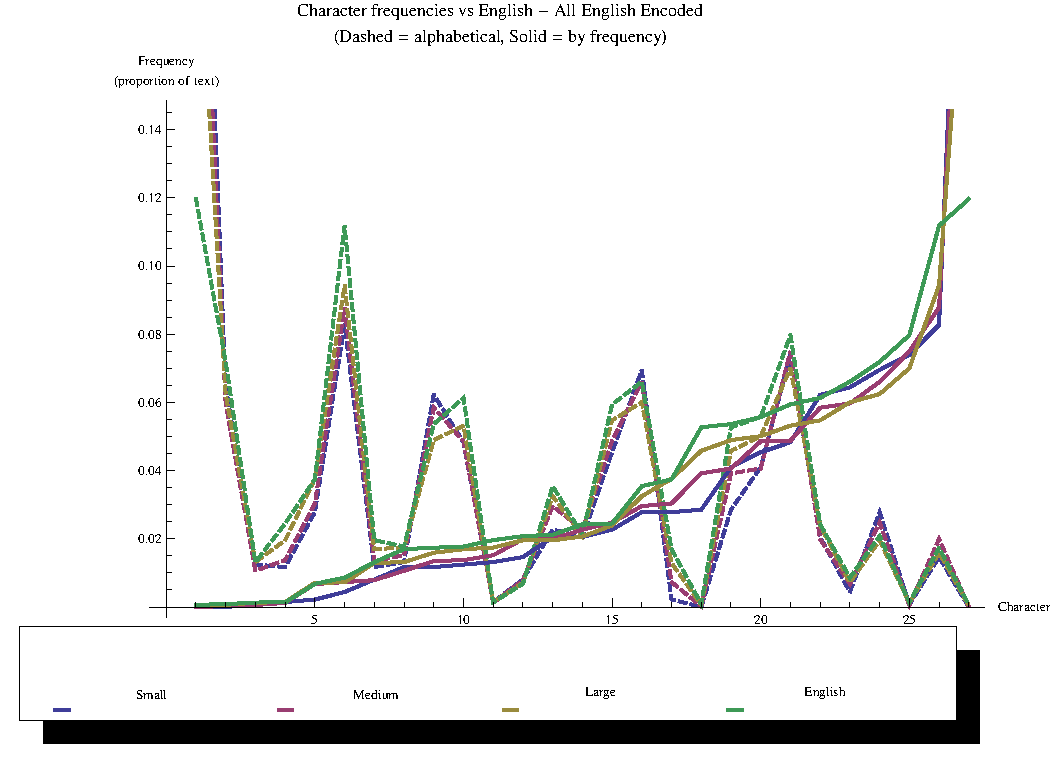
\includegraphics[width=4in]{figures/markov-a.pdf}
%\end{figure}
%\begin{figure}
%\centering
%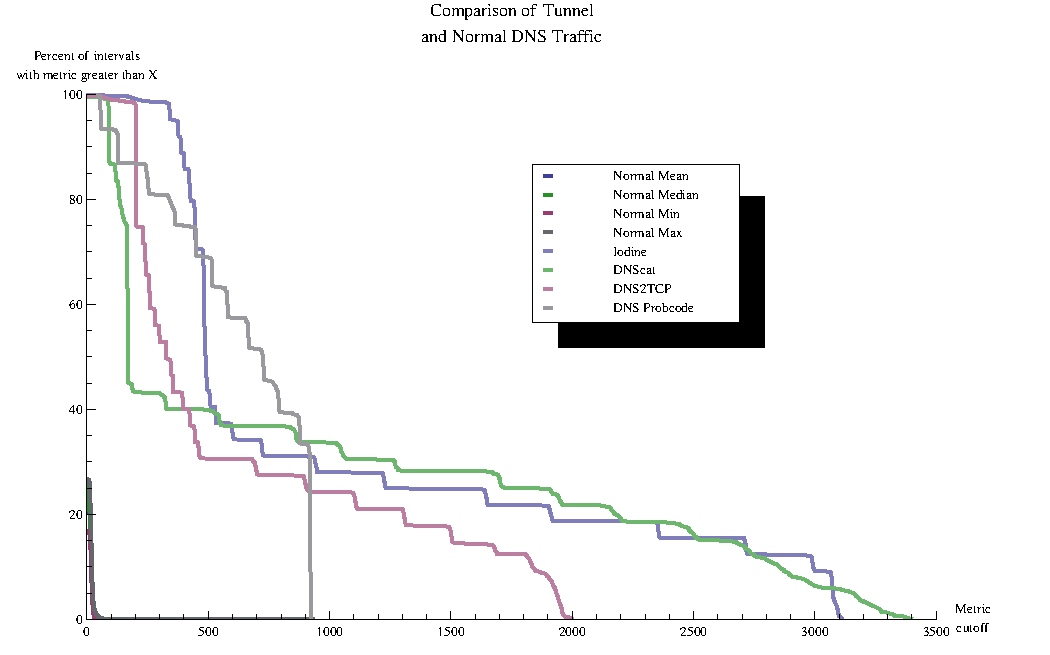
\includegraphics[width=4in]{figures/metric-tun_v_norm.pdf}
%\end{figure}
%\begin{figure}
%\centering
%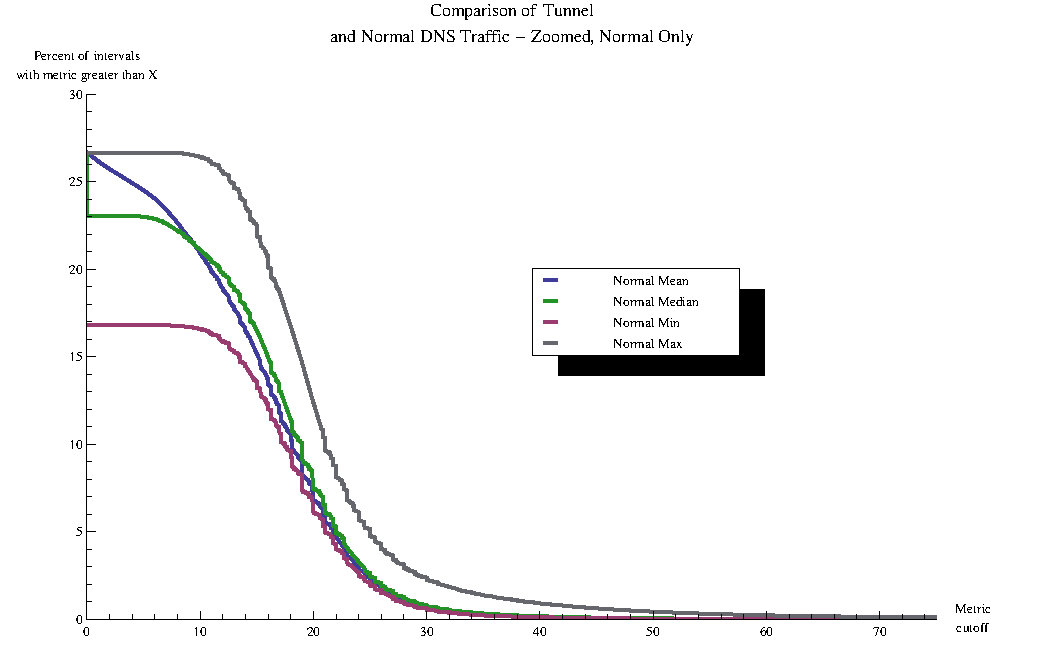
\includegraphics[width=4in]{figures/metric-tun_v_norm-norm-zoom.pdf}
%\end{figure}
%\begin{figure}
%\centering
%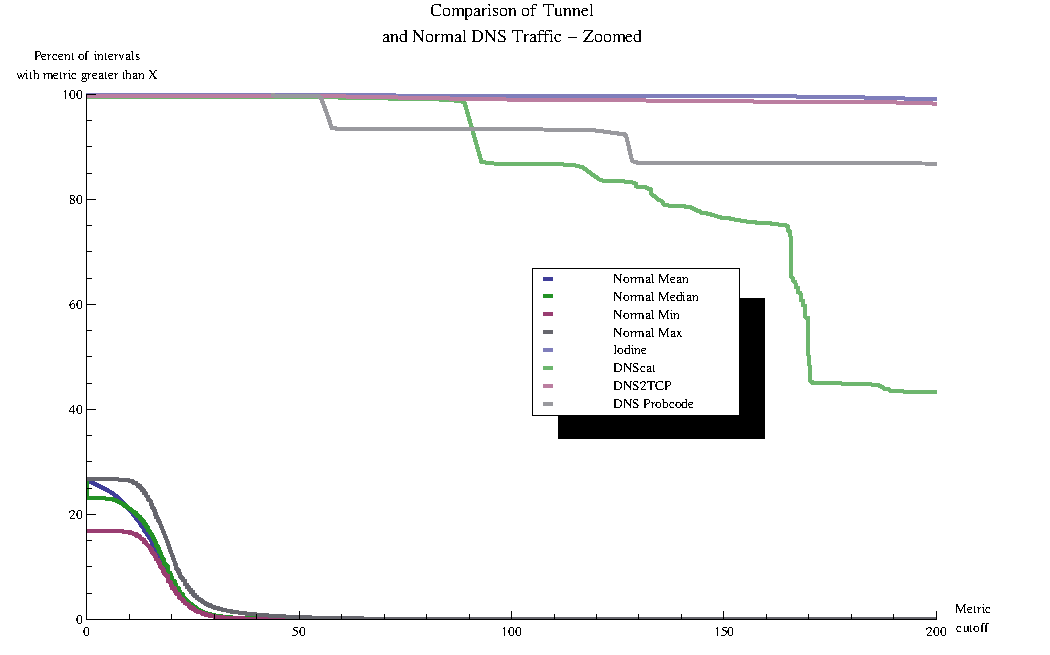
\includegraphics[width=4in]{figures/metric-tun_v_norm-zoom.pdf}
%\end{figure}
%\begin{figure}
%\centering
%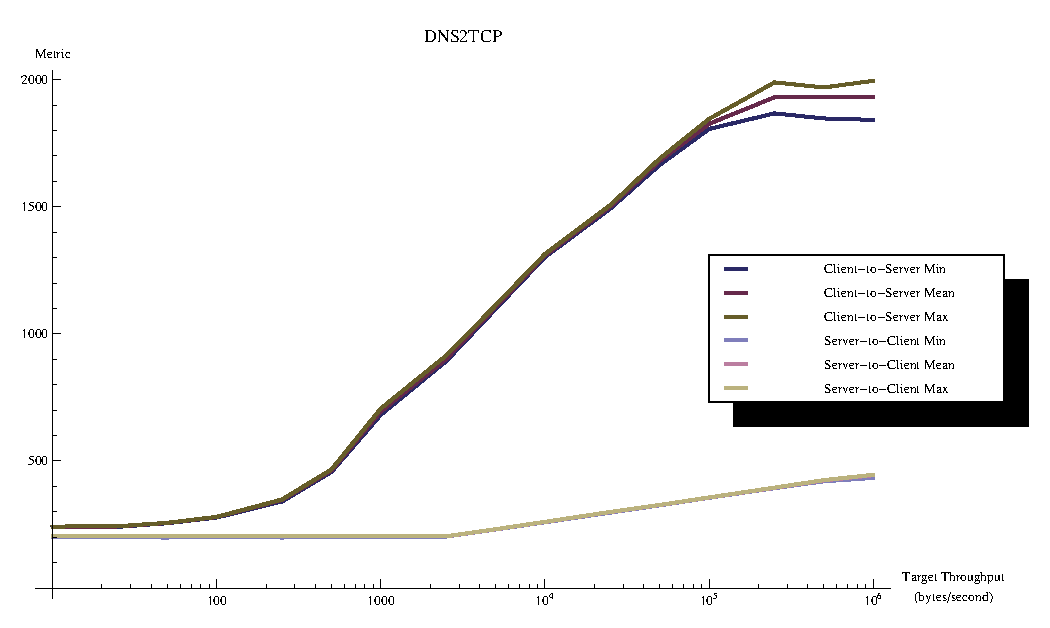
\includegraphics[width=4in]{figures/metric-tun-dns2tcp.pdf}
%\end{figure}
%\begin{figure}
%\centering
%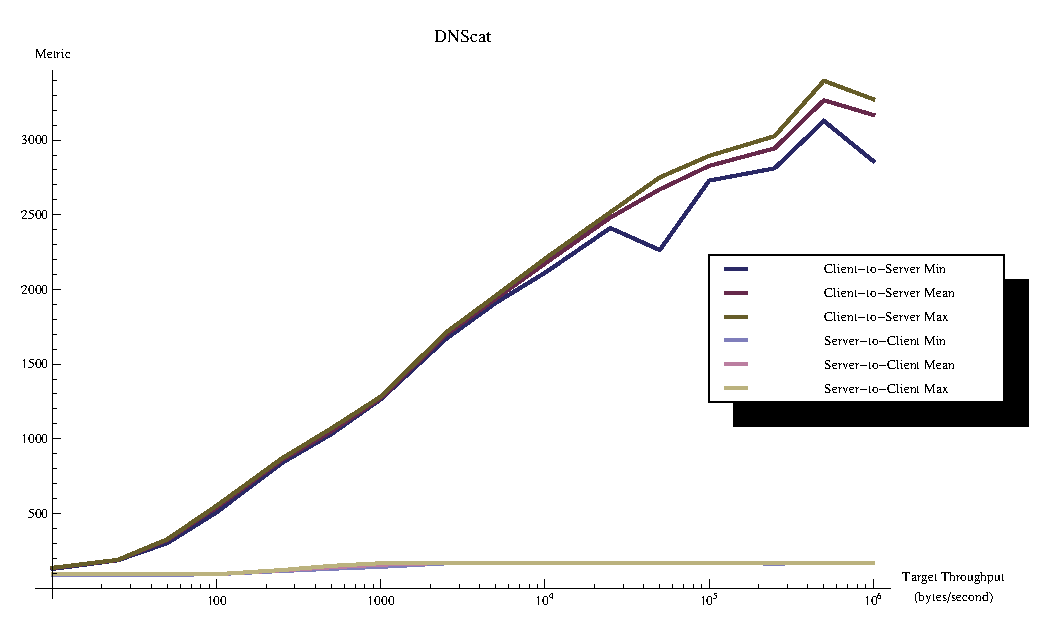
\includegraphics[width=4in]{figures/metric-tun-dnscat.pdf}
%\end{figure}
%\begin{figure}
%\centering
%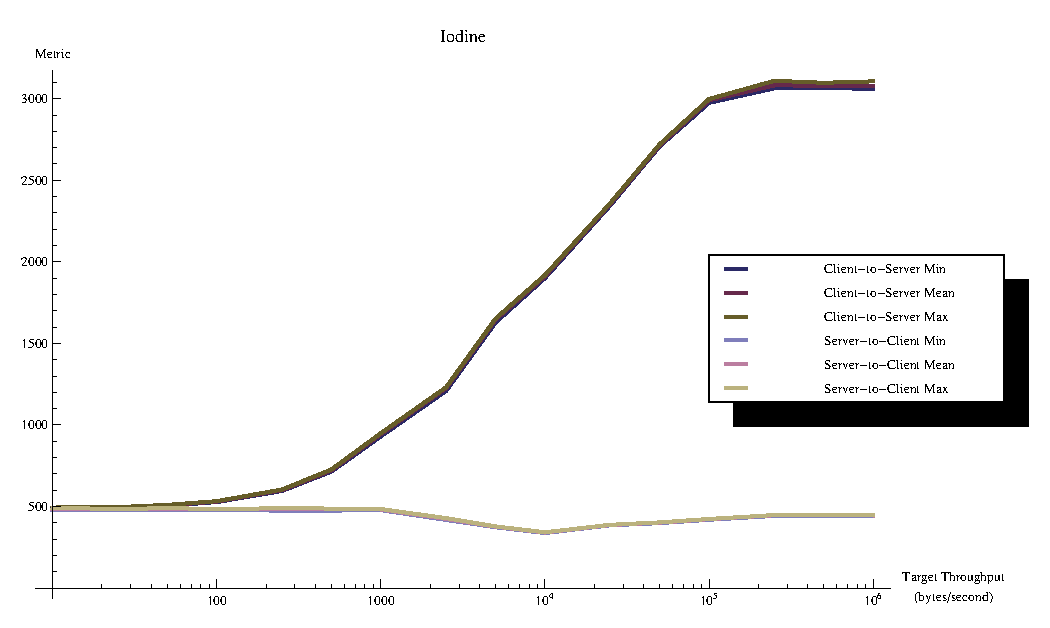
\includegraphics[width=4in]{figures/metric-tun-iodine.pdf}
%\end{figure}
%\begin{figure}
%\centering
%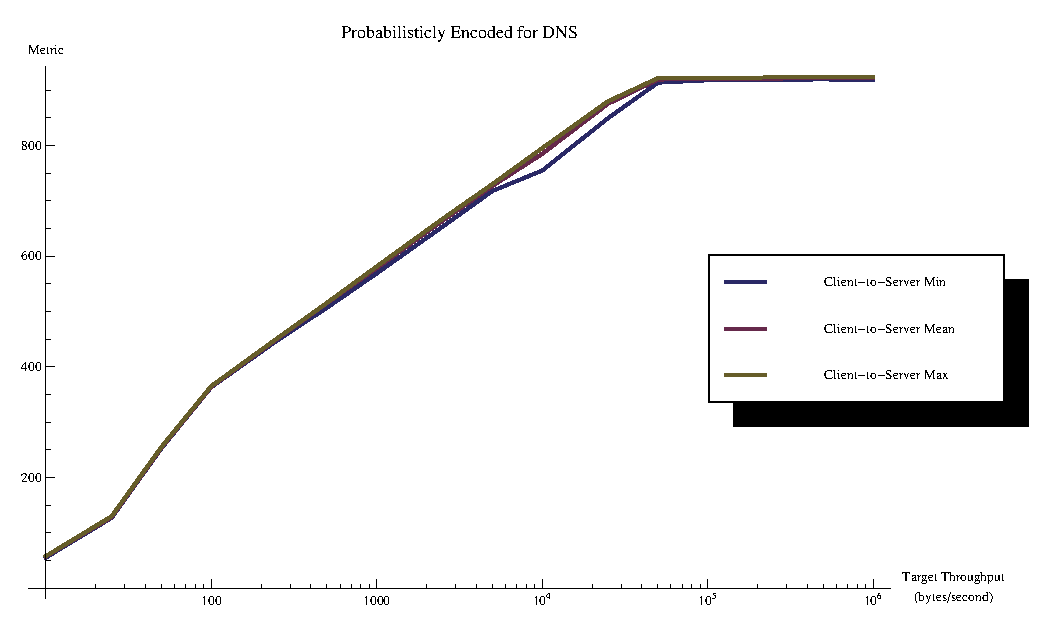
\includegraphics[width=4in]{figures/metric-tun-probdns.pdf}
%\end{figure}
%\begin{figure}
%\centering
%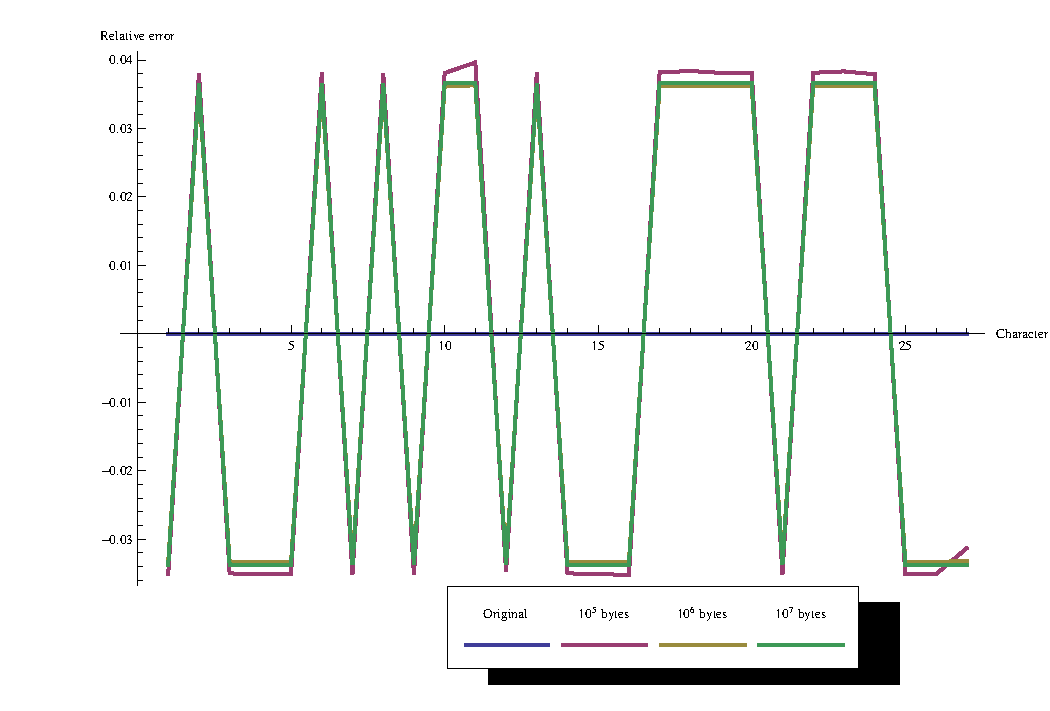
\includegraphics[width=4in]{figures/pdf_convergence.pdf}
%\end{figure}
%\clearpage
%\begin{figure}
%\centering
%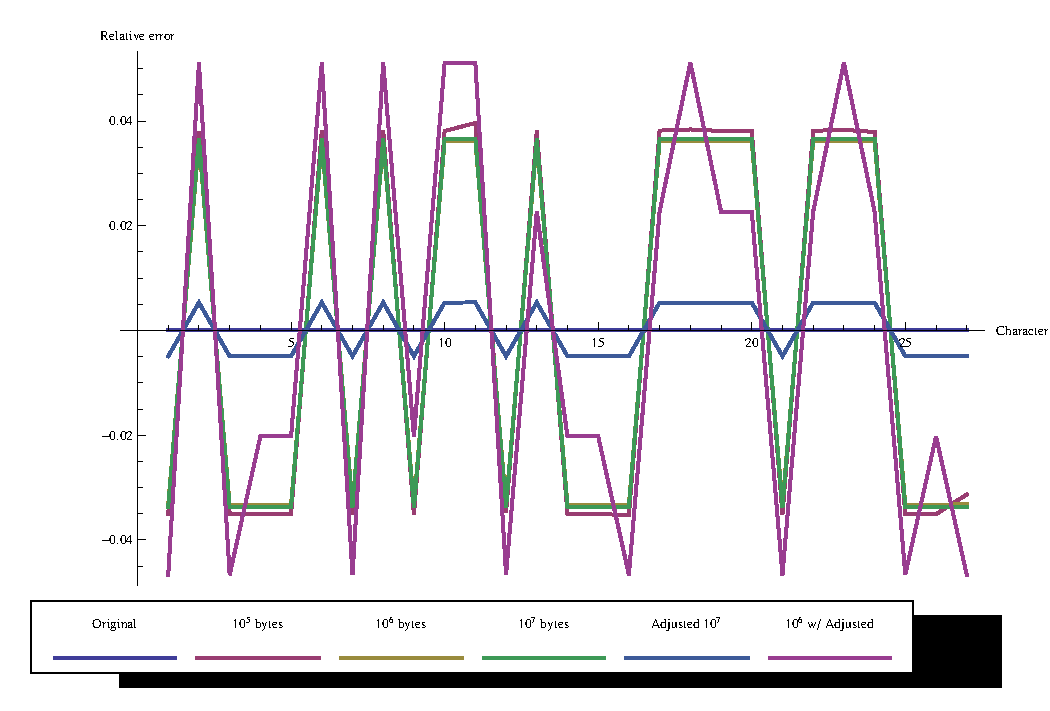
\includegraphics[width=4in]{figures/pdf_convergence_adjusted.pdf}
%\end{figure}
%\begin{figure}
%\centering
%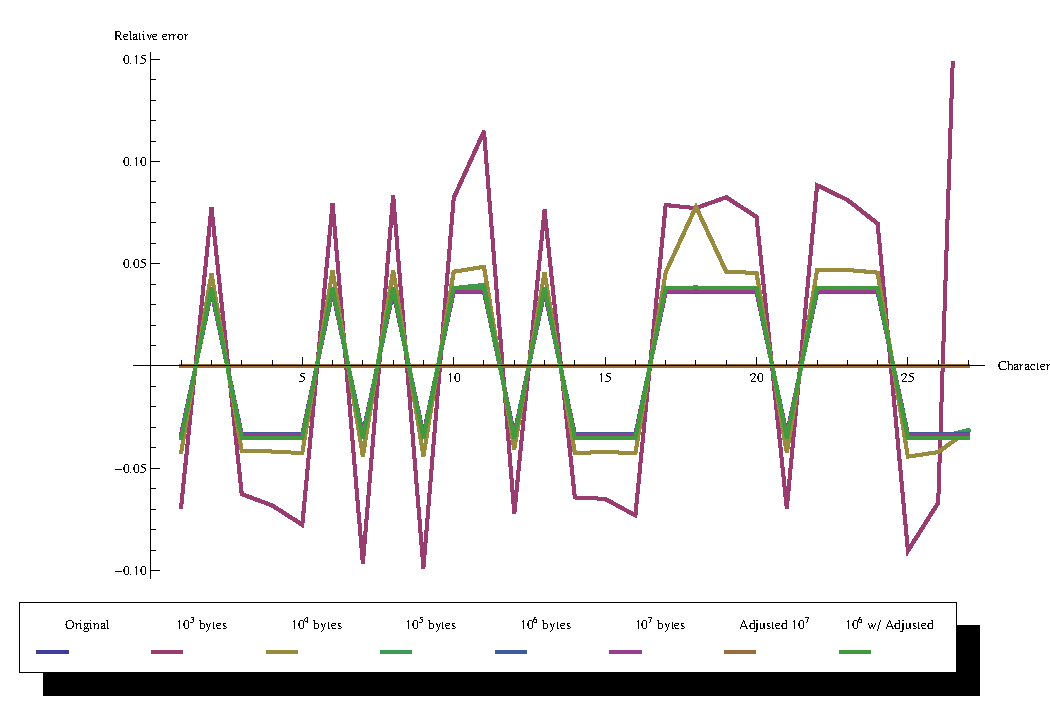
\includegraphics[width=4in]{figures/pdf_convergence_adjusted2.pdf}
%\end{figure}
%\begin{figure}
%\centering
%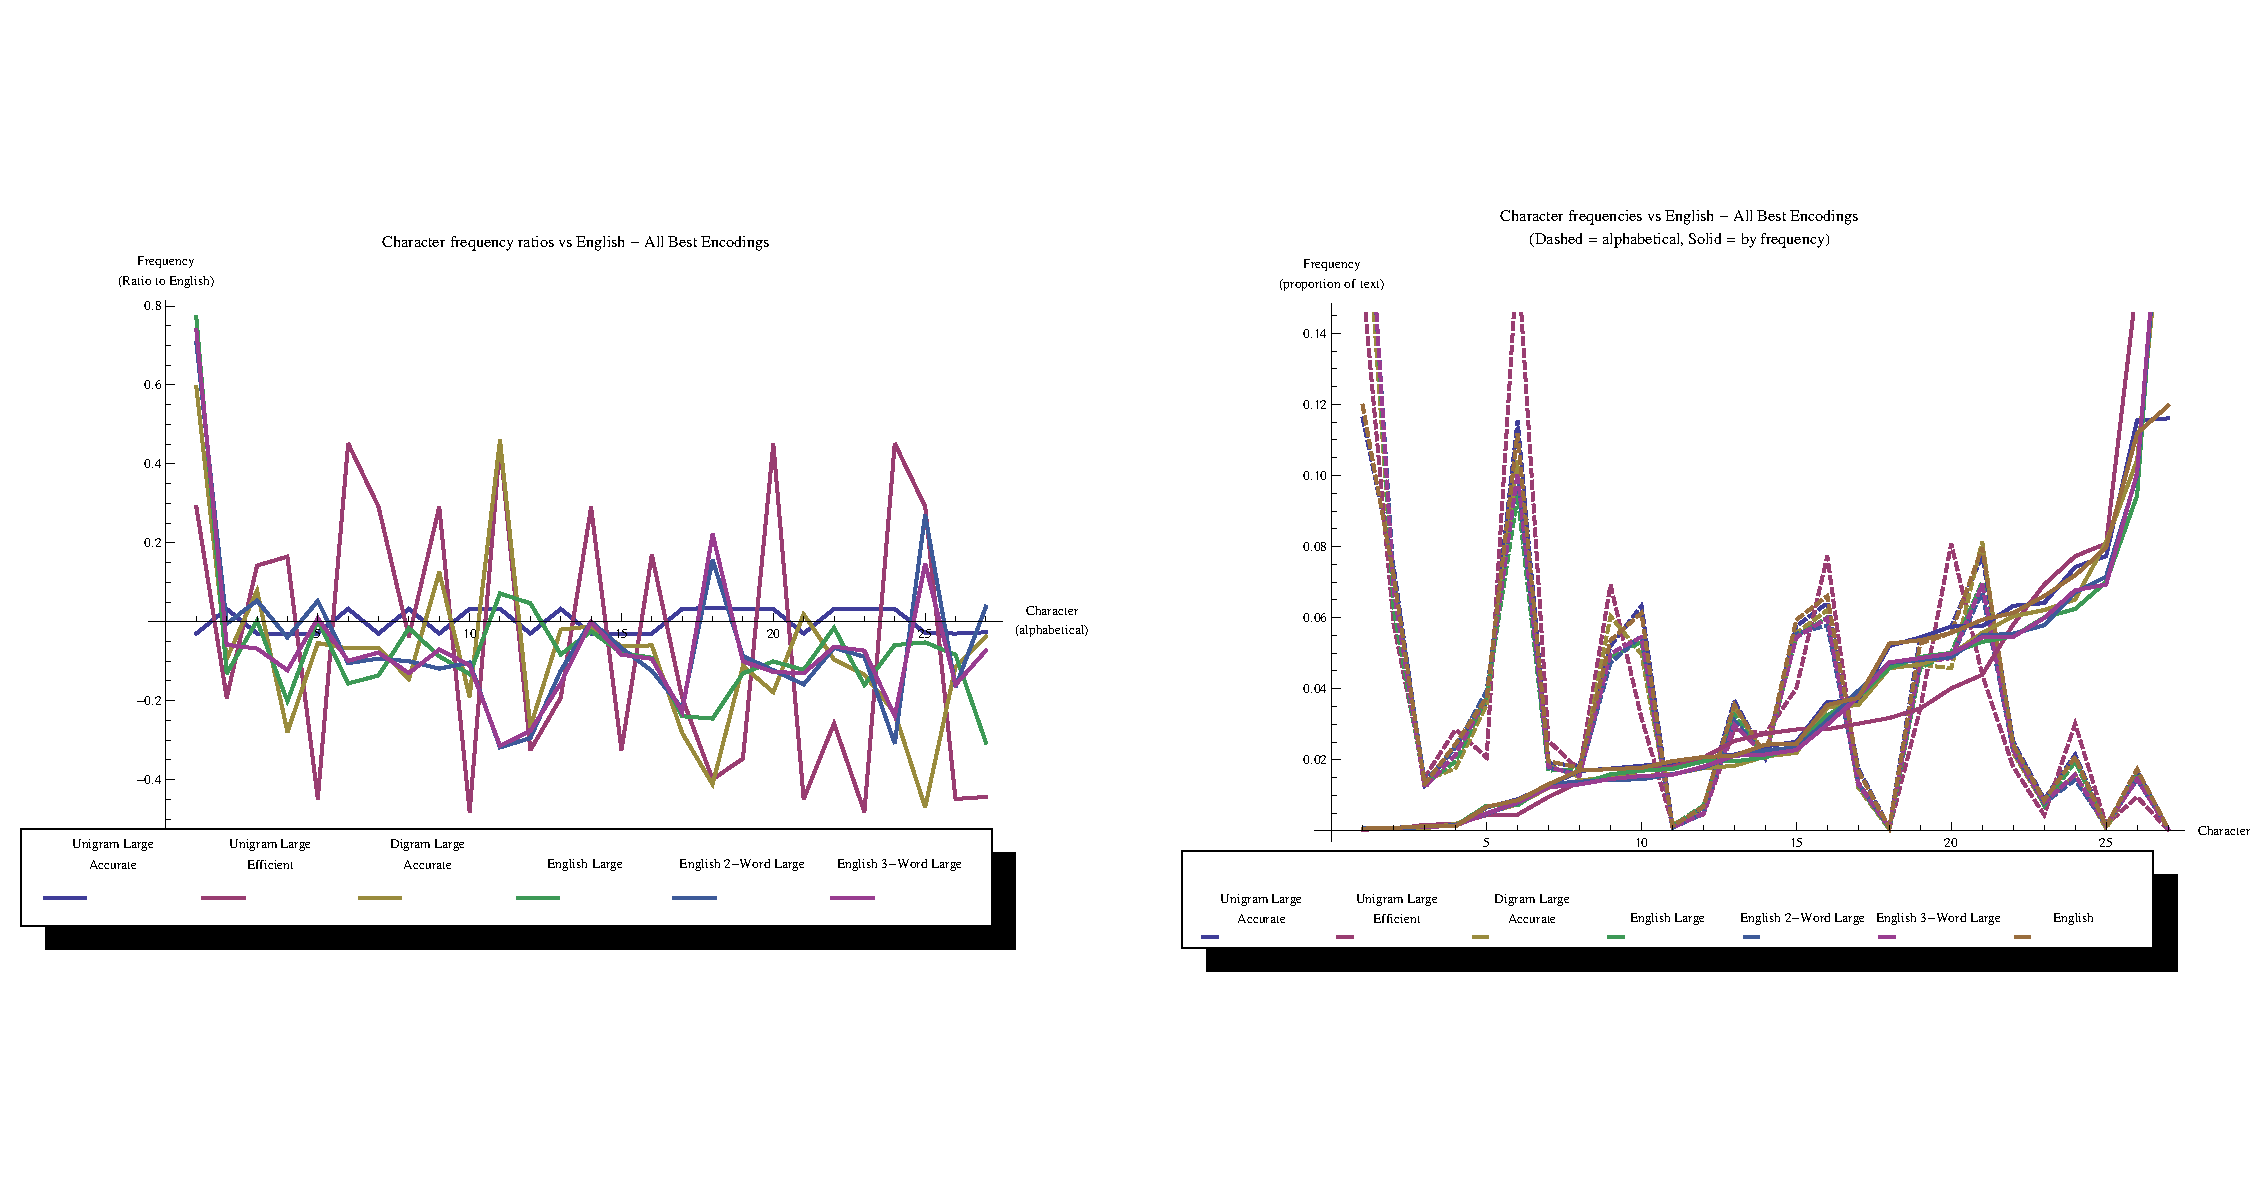
\includegraphics[width=4in]{figures/plots_best.pdf}
%\end{figure}
%\begin{figure}
%\centering
%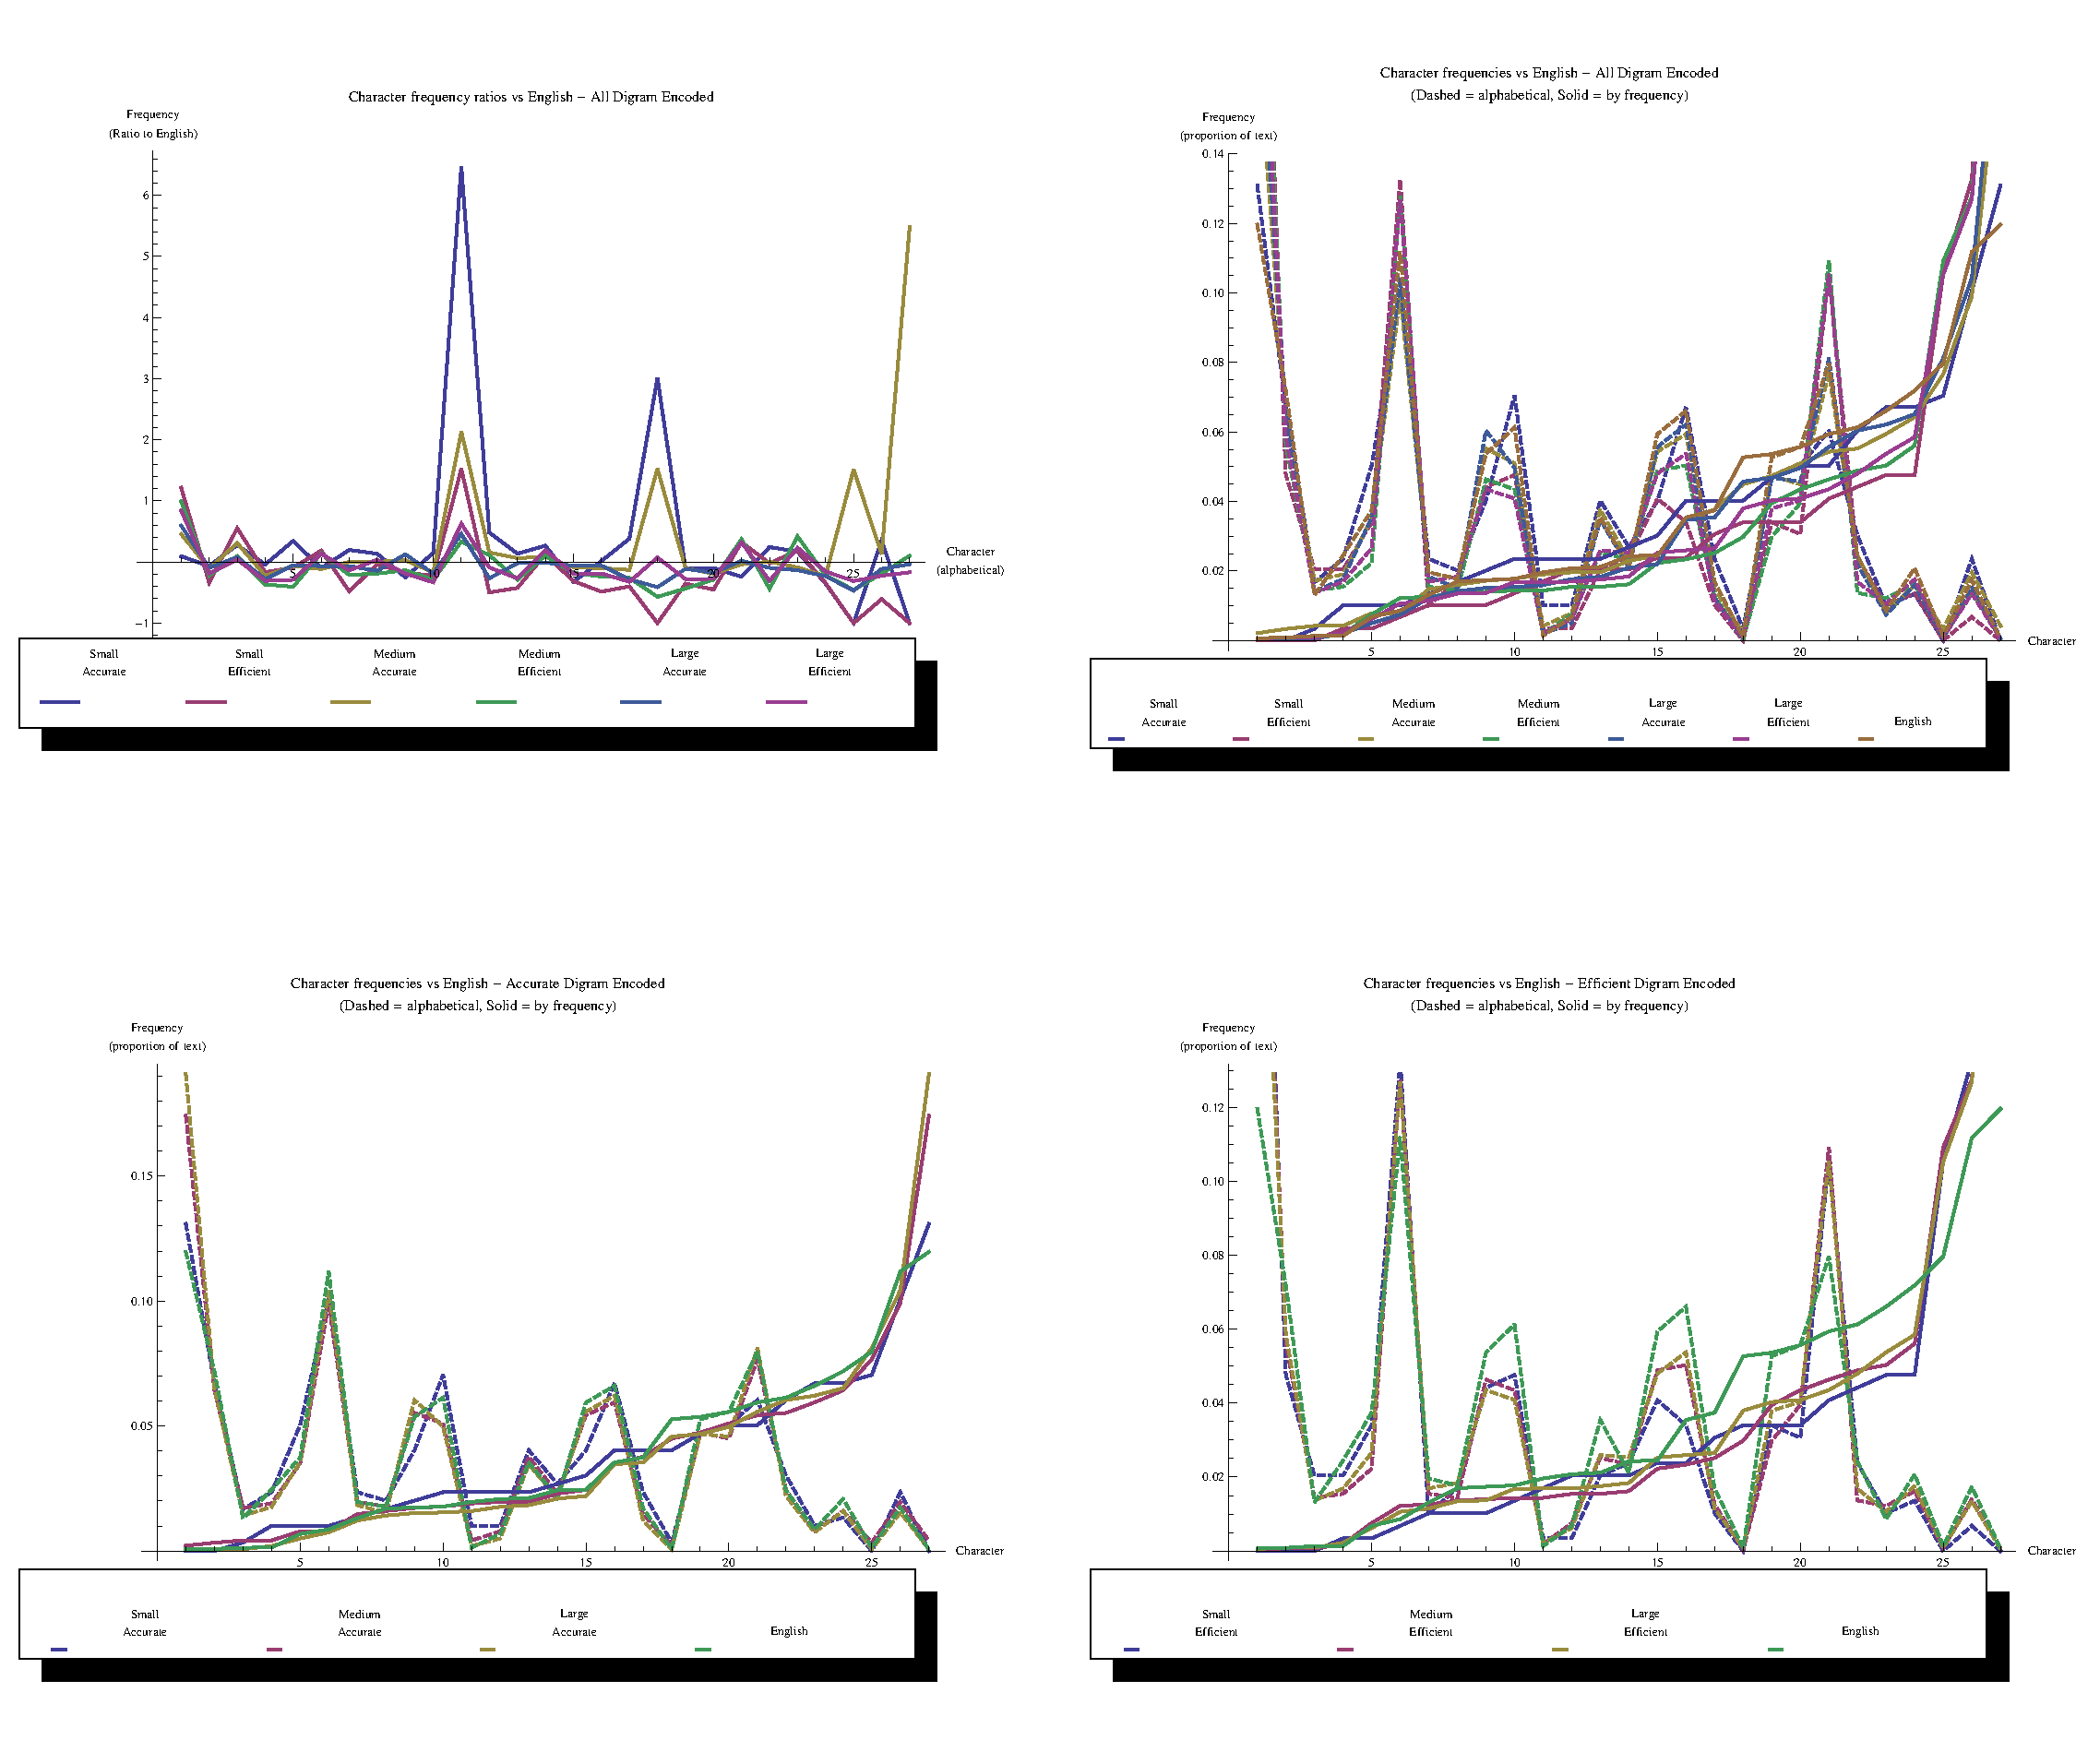
\includegraphics[width=4in]{figures/plots_digram.pdf}
%\end{figure}
%\begin{figure}
%\centering
%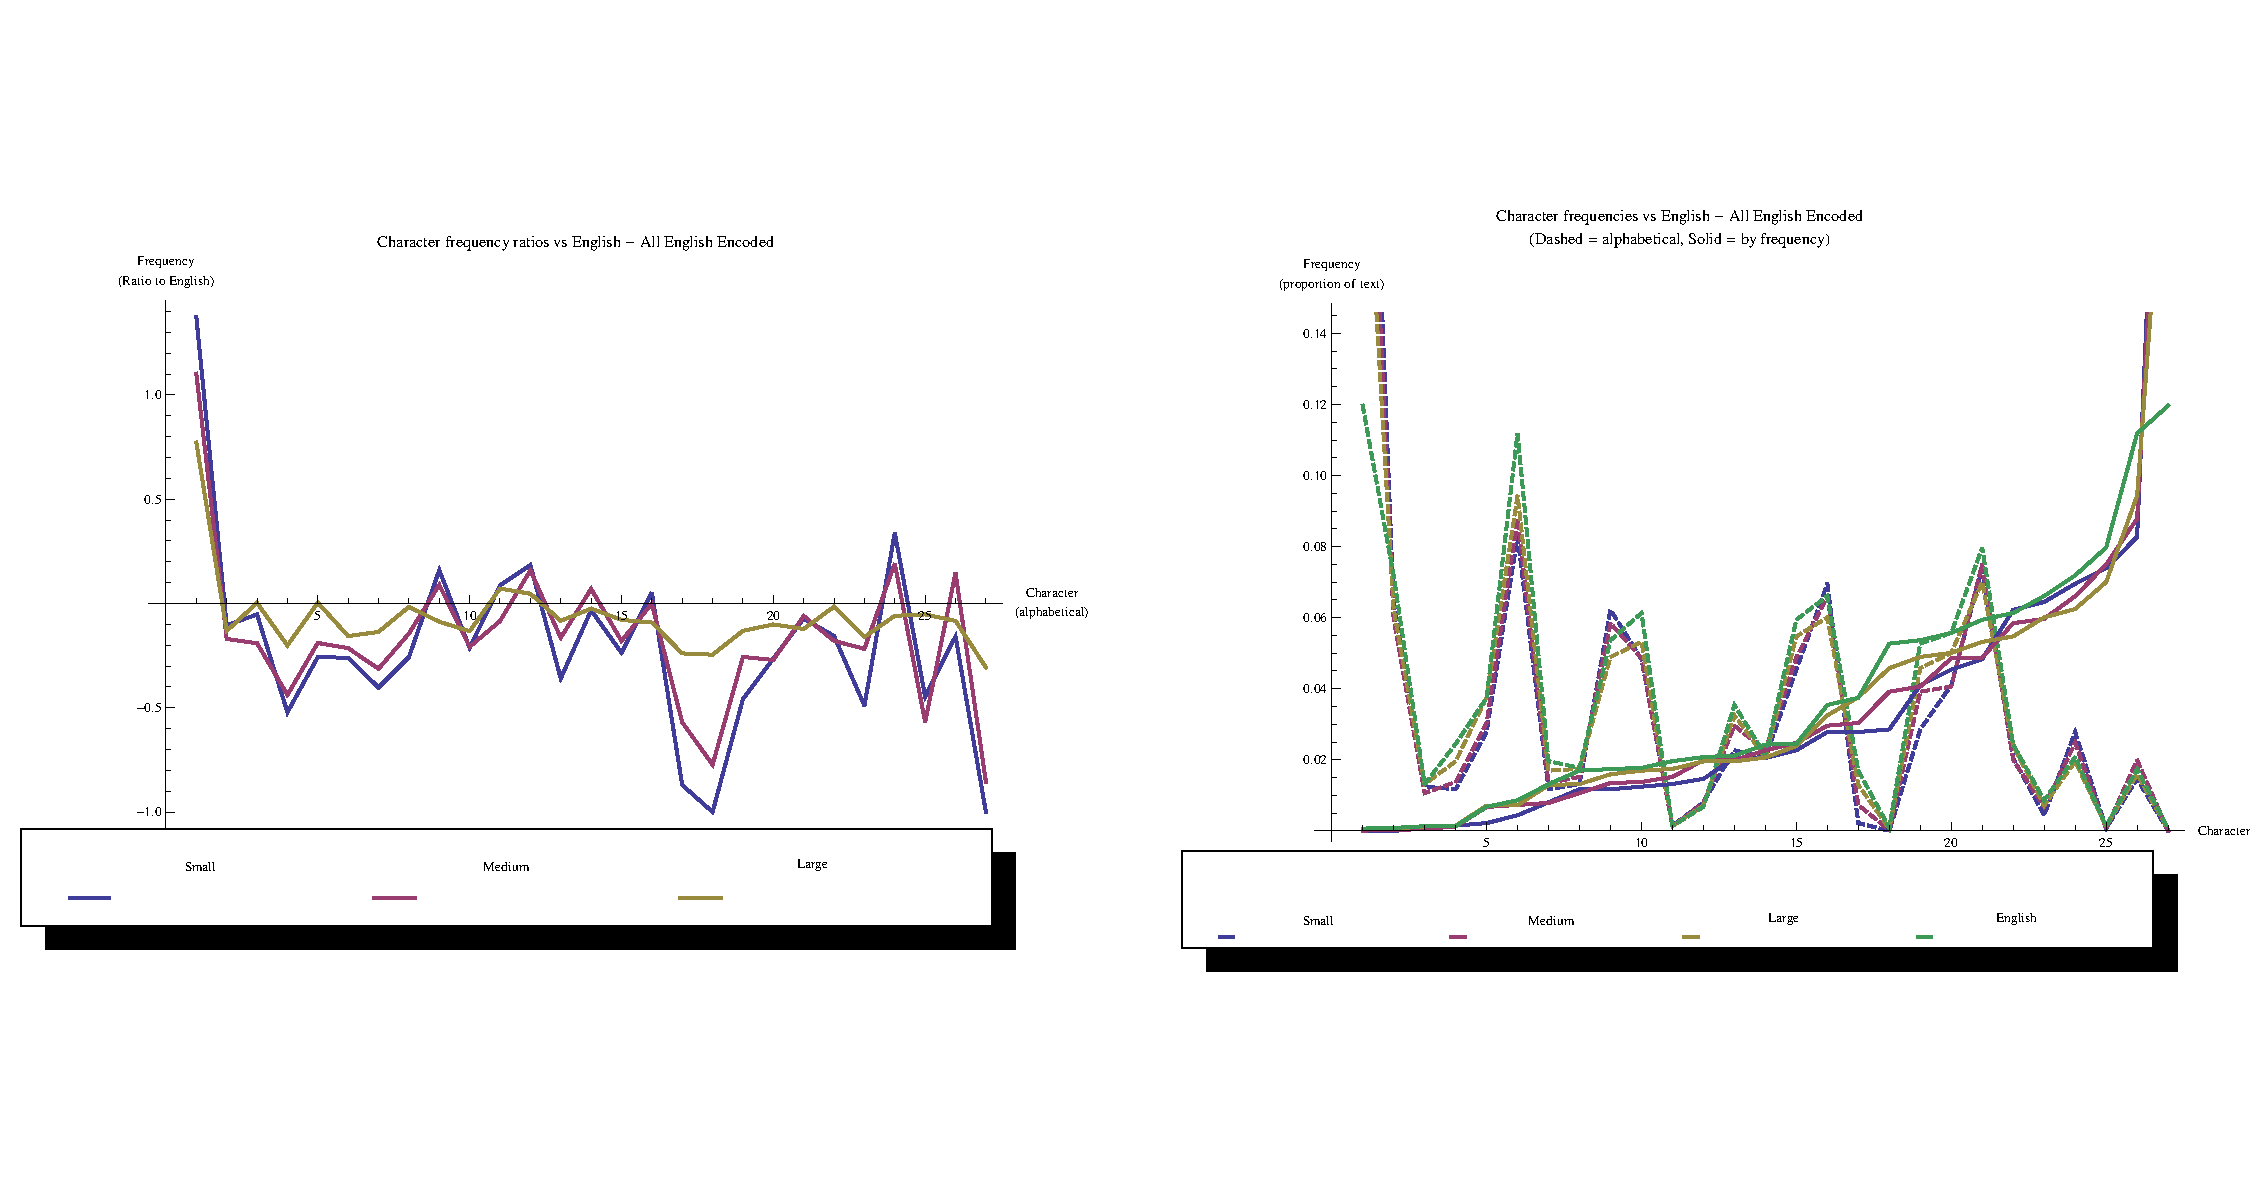
\includegraphics[width=4in]{figures/plots_markov1.pdf}
%\end{figure}
%\begin{figure}
%\centering
%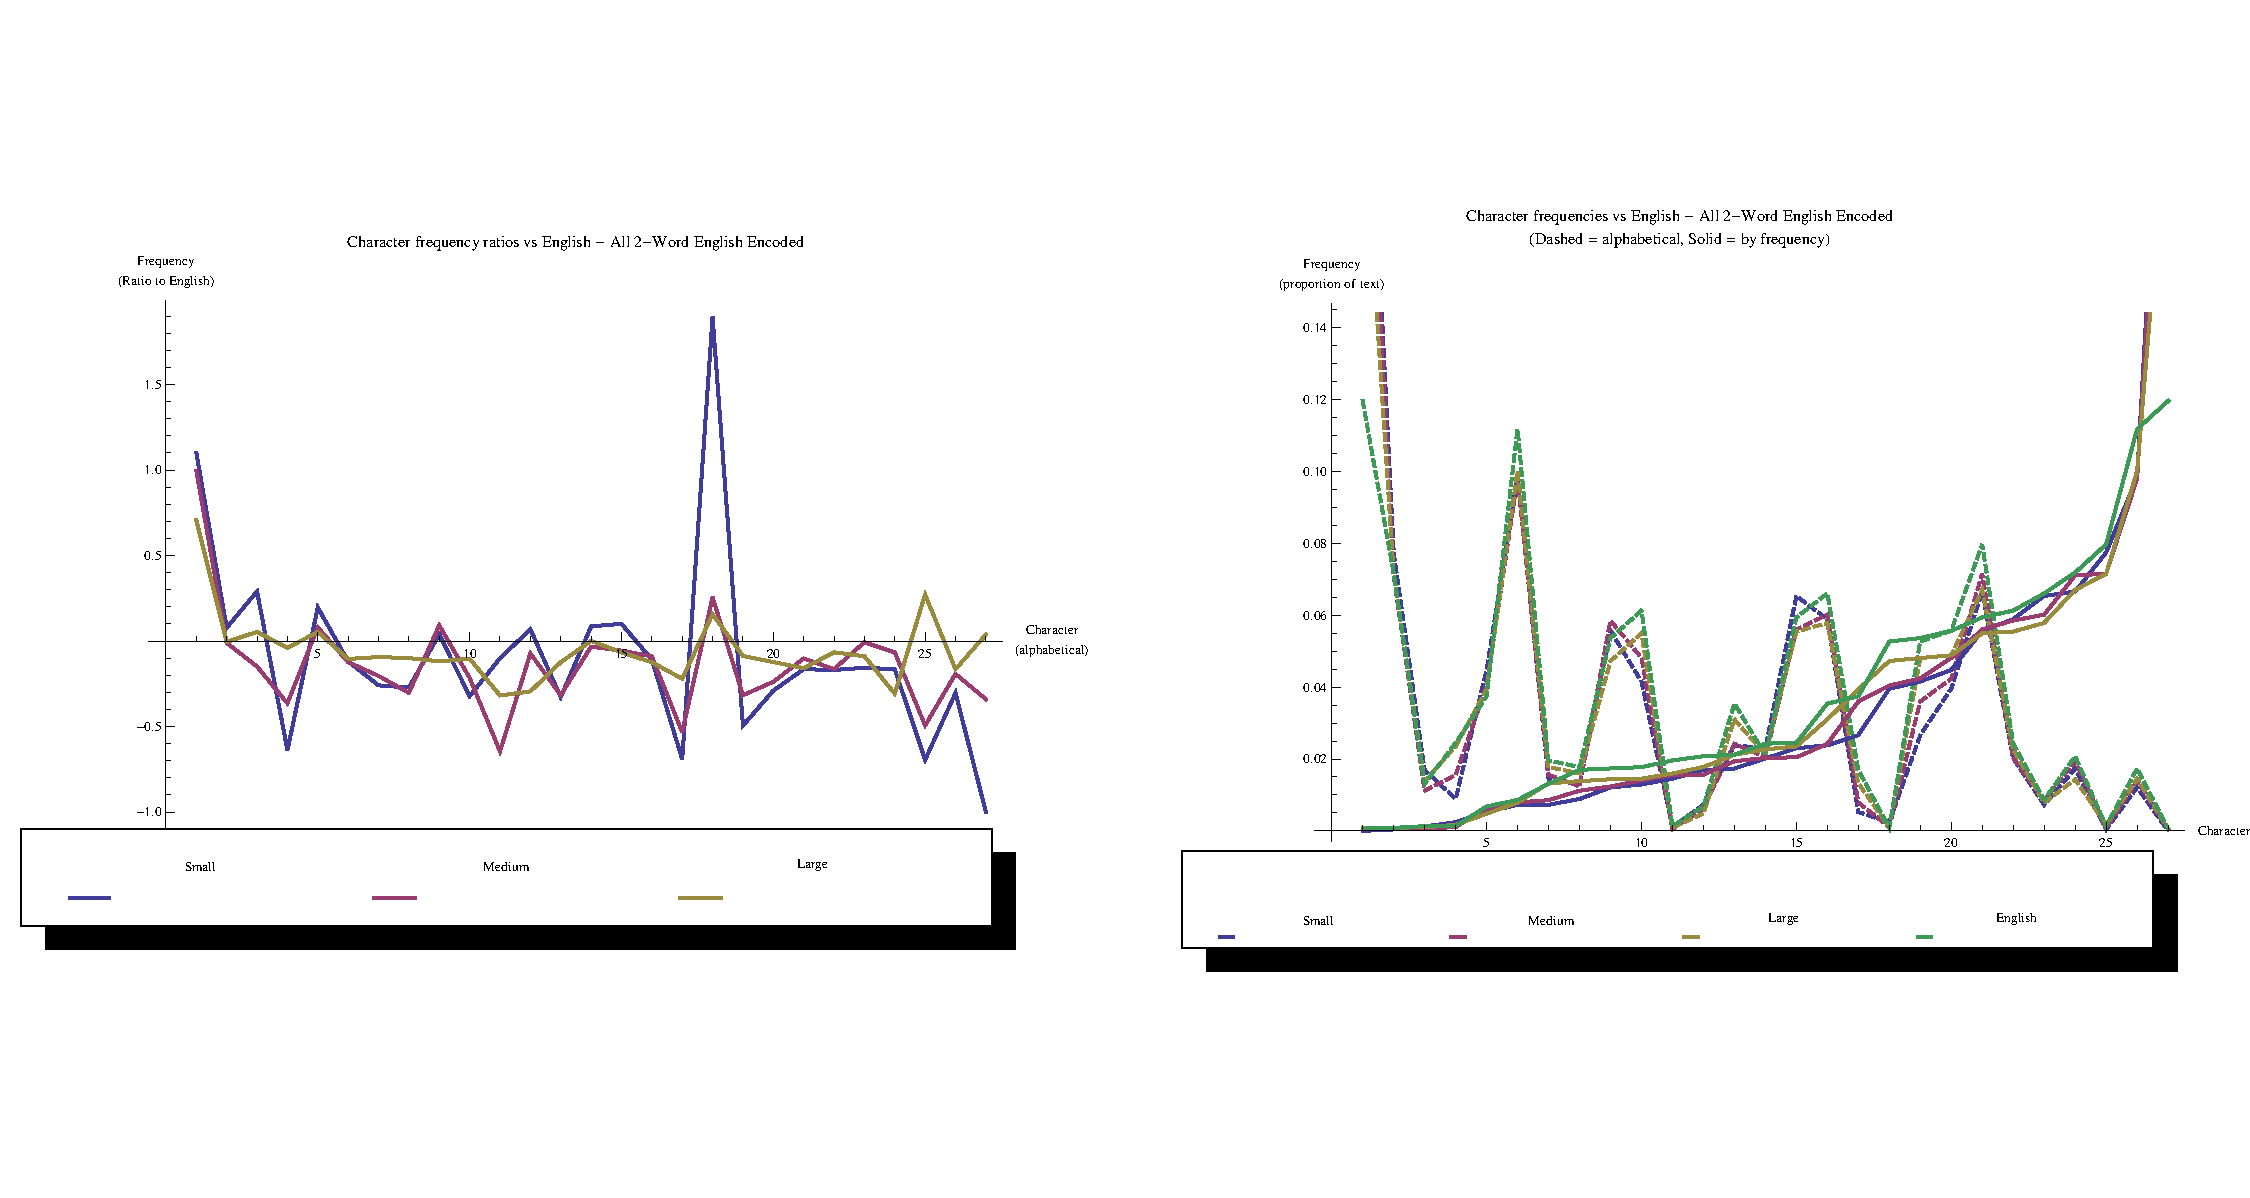
\includegraphics[width=4in]{figures/plots_markov2.pdf}
%\end{figure}
%\begin{figure}
%\centering
%\includegraphics[width=4in]{figures/plots_markov3.pdf}
%\end{figure}
%\begin{figure}
%\centering
%\includegraphics[width=4in]{figures/plots_unigram.pdf}
%\end{figure}
%\begin{figure}
%\centering
%\includegraphics[width=4in]{figures/tunnels-freqabs.pdf}
%\end{figure}
%\begin{figure}
%\centering
%\includegraphics[width=4in]{figures/tunnels-freqrel.pdf}
%\end{figure}
%\clearpage
%
%\clearpage



\begin{appendices}
\chapter{Properties of the Network Capture}
\label{appendix-capturestats}

The packet capture used to represent real world data was performed in cooperation with Merlin, an ISP in Manitoba for educational institutions.

\begin{table}[h]
\centering
\begin{tabular}{ l l }
File name:           &data1.udp53.pcap\\
File type:           &Wireshark/tcpdump/... - libpcap\\
File encapsulation:  &Ethernet\\
Packet size limit:   &file hdr: 65535 bytes\\
Number of packets:   &1035425650\\
File size:           &156484681395 bytes\\
Data size:           &139917870971 bytes\\
Capture duration:    &1915055 seconds\\
Start time:          &Thu Nov  4 15:05:58 2010\\
End time:            &Fri Nov 26 18:03:33 2010\\
Data byte rate:      &73062.06 bytes/sec\\
Data bit rate:       &584496.51 bits/sec\\
Average packet size: &135.13 bytes\\
Average packet rate: &540.68 packets/sec\\
SHA1:                &6fb043f37e659d9a65a45b5c8074d55eae386600\\
RIPEMD160:           &4aba72d43f5726f0a8576f35d60845f895080a43\\
MD5:                 &32956ef8efe5c3873226386e1608561a\\
Strict time order:   &True\\
\end{tabular}
\caption[Packet Capture Statistics from \emph{capinfos}]{Statistics and information as reported by Wireshark's utility \emph{capinfos} on the real world packet capture..}
\label{TABLE_capinfos}
\end{table}

While the capture file contains over one billion total packets, only 339,321,911 (or $32.7\%$) of the packets represent valid DNS traffic.

\begin{figure}
\centering
\includegraphics[width=\textwidth]{figures/pcap-tpb.pdf}
\caption[Throughput in Bytes per Second of Packet Capture]{Throughput in bytes per second of the packet capture, with each sample being the average throughput over ten-second windows.}
\label{cplot}
\end{figure}

\begin{figure}
\centering
\includegraphics[width=\textwidth]{figures/pcap-tpp.pdf}
\caption[Throughput in Packets per Second of Packet Capture]{Throughput in packets per second of the packet capture, with each sample being the average throughput over ten-second windows.}
\label{cplot}
\end{figure}


%\chapter{Testing Software and Scripts}

%\chapter{Testing Environment}
%\label{appendix-setup}

\chapter{Probabilistic Encoding}
\label{appendix-probcode}
Several detection methods in
the literature involve examining the character distribution in the queries, or
responses, of DNS packets. These approaches compare the distributions obtained
from the traffic being analyzed, and compare them to a known distribution that
can be considered normal. If there is a sufficiently significant measurable
difference, then the packet is flagged as anomalous.

If it were possible for a DNS tunnel to encode its output in order to match the
distribution that these detection methods consider normal, then it would be
possible for it to evade detection by masquerading as benign DNS traffic. These
detection methods assume that the output of a DNS tunnel will have high entropy
(due to compression and/or encryption) and/or span a wide range of character
values, whereas normal traffic does not have these features. The solution to
this problem becomes one of converting a high entropy source into a lower entropy
encoding in a way that the high entropy stream can be recovered from the low
entropy encoding, where the low entropy encoding has a specific distribution of
characters.

A proof-of-concept tool was written in C that performs precisely this task. The
tool takes, as input, what it assumes to be a high entropy source\footnote{Since
any source can be used to produce a high entropy source through encryption or
compression, this is considered a safe assumption and limitation.} and a
configuration file that describes the desired output distribution.

\section{Sample Encoding - English Unigrams}

A sample encoding is given using the english character
frequency distribution with the character distribution table used given in table
\ref{TABLE_unigrams}. In order to ensure that interested parties can verify this
output, the source high-entropy data is contained in table
\ref{TABLE_encodingsource}. A data matrix image of the same base64 encoding is
also given in figure \ref{FIGURE_encodingsource}. This can be converted back to
the original source via the standard Unix command line tool \emph{base64}. The
output of the encoder using english character frequencies and the given input
data is shown in table \ref{TABLE_encodingoutput-unigram}. It is important to observe
that the output produced does not resemble typical English text and can be easily
detected by any software that performs analysis on higher level characteristics.
Such distinguishing characters include, but are note limited to, digrams, trigrams,
and the existence of English words.

\begin{table}
\centering
\begin{tabular}{ | c | c || c | c | }
Character&Count&Character&Count\\
\hline
$<$\emph{space}$>$&0.11965  &  u&0.0242803\\
e&0.111823 &  m&0.0211814\\
t&0.0797253&  w&0.0207765\\
a&0.0718989&  f&0.0196144\\
o&0.0660886&  g&0.0177392\\
i&0.0613258&  y&0.0173783\\
n&0.0594154&  p&0.0169821\\
s&0.0557003&  b&0.013135\\
h&0.0536491&  v&0.00860991\\
r&0.0527071&  k&0.00679637\\
d&0.0374417&  j&0.00134695\\
l&0.0354345&  x&0.00132054\\
c&0.0244916&  q&0.000836341\\
       &    &  z&0.000651466\\
\end{tabular}
\caption[English Character Frequency]{Probability distribution used for english character frequency in the sample encoding and decoding.}
\label{TABLE_unigrams}
\end{table}

\begin{table}
\begin{verbatim}
HEzQcP9uxPOzeOB1SfRP+DQ7x3X5dTA1WF3vpcnO5kgLQQEP7xnUrnUy7U8ISNdbNQd+8da64+Ci
nNBRvu3TRlG0KJvLzb6QDBWqxVfa4VeAU+cSvj+uzoajp2F0jd5/csHxJQlguoeqT76pq8oStoLG
3k48PZWuebgweZx5KdxAgUfN7/kvzwBzG7O+9B7J/O8y6BfGz6In0H+LuDCOsFqMljljX3SkgJq/
yPka52SDxa3D4GXecj9d
\end{verbatim}
\caption[Encoding Sample - Source]{The base64 encoding of the binary data used for the sample encoding.}
\label{TABLE_encodingsource}
\end{table}

\begin{figure}
\centering
\includegraphics[width=4in]{figures/encoding_source.png}
\caption[Encoding Sample - Source (data matrix)]{The base64 encoding of the binary data used in the sample encoding, represented in a data matrix image.}
\label{FIGURE_encodingsource}
\end{figure}

\begin{table}
\begin{verbatim}
" mfeo  hnhaeeeewsao os eewk es fsemroh eeeewthesdre s sol sreese ea hrzltse
wesrnyemnpaoonef  ht   hsheawnfdemue stntleewth    home esaiu s feesgealne seaoa
hlhyp hmb ewaaeesdubotongtnploaanewefochd htugeside s oeesi   fptsmr
hweeeesoltsnahao esde hgmuo weeeeewyl  haoesroo     frmeshtieest ewad svikefui
hnceslphstestidau eeahl hrosoan wrthaa ft  heabpeeses eeeeewrsn    hrlucne ewr
esesooc eeeeeewsqe eewefgeesng est f eeeeewlhhae hgao hiuggnrrancewgmob
hdreeesgopesuoamyufiolisx esrrsloaeewtse"
\end{verbatim}
\caption[Encoding Sample - Output]{The encoded form of the binary data according to English character frequencies.}
\label{TABLE_encodingoutput-unigram}
\end{table}

% Efficiency numbers
% ==================
% Unigram
%   Efficient 0.417057 v 256946 0.06682579831758034750036661712845
%   Accurate 0.300548 v 332774 0.00014558032328364780948779390679
% Digram
%   Efficient 0.410661 v 270396 0.90056751440933662212073829206813
%   Accurate 0.280415 v 355834 0.0021880889

Analyzing the frequencies of the output shows that it closely approximates
english character frequencies. A larger sample of random data (one hundred
thousand bytes) was also encoded, and its output analyzed as well. The small
sample, the large sample, and actual english character frequencies are displayed
together in figure \ref{FIGURE_frequencies-bytop}. As is evident from the combined plots of the
various distributions, there does not exist a clear distinction between them and
thus it becomes very difficult to perform automated classification when
information is encoded using this tool.

\begin{landscape}
\begin{figure}
\centering
\includegraphics[width=1.15\textwidth]{figures/plots_unigram.pdf}
\caption[Plot of Character Frequencies]{The character frequencies of the small and large encoded samples using both accurate and efficient encoding, as well as the English target distribution sorted by character.}
\label{FIGURE_frequencies-bytop}
\end{figure}
\end{landscape}

\subsection{Technical Details} The probabilistic encoder is open-source and
freely available, licensed under the Mozilla Public License version 2 which is
GPL compatible. The source code is available at \cite{probcodesrc} for download
and use under the MPL2 license terms. The source code compiles on Unix and other
POSIX based systems sych as Cygwin on Windows as well as non-POSIX platforms such as Visual Studio on Windows.

The encoding and decoding processes can be broken up into two steps; probability
distribution analysis followed by the encoding or decoding. The analysis of the
distribution is the same for both the encoding and decoding operations, however
the encoding operation is somewhat more involved than the decoding operation
from an algorithmic point of view.

The probability distribution is analyzed in order to map each element of the
distribution (character, word, etc$\ldots$) to a string of bits. An assumption
is made that all bit strings of a given length are equally likely to appear in
the high-entropy source, and this places a constraint in the output PDF; the
most frequent symbol cannot be more frequent than the most frequent symbol in
the high-entropy source. That is, no symbol in the output distribution can have
a frequency above 50\%. This is considered a fair assumption since in English,
the most common letter has a frequency of approximately 11\%.

The mapping from symbol to bit string is done by sorting the distribution from
most to least frequent, and then selecting a shortest available bit string of a
length that has an expected occurrence rate not less than the symbol's
occurrence rate in the output distribution. For example, the bit string to
symbol mapping for the English unigram encoding sample is given in Table
\ref{TABLE_unigrammapping} along with the approximate frequency of the letters
in English text.

Observe that it is possible to make a tradeoff between encoding accuracy (that
is, how accurately the output matches the desired distribution) and encoding
efficiency (that is, the ratio between output and input size with higher ratios
indicating a less efficient encoding) by tuning the bit string mapping. More
accurate mappings result from choosing shorter bit strings (table
\ref{TABLE_unigrammapping_acc} chooses the shortest possible bit string mappings and
achieves an efficency factor of approximately 3.3) with more efficient mappings
sacrificing accuracy for efficiency. Figure \ref{FIGURE_frequencies-bytop} shows
the frequencies of the English target distribution along with the most efficient
encoding and the most accurate encoding. The efficient coding (shown in table \ref{TABLE_unigrammapping_eff}) in that figure
achieves a factor of 2.4 compared to the accurate encoding's factor of 3.3.
The efficiency factors represent the ratio of bytes in the output compared to
bytes in the input.

Once the mapping, and various lookup tables built, have been built the
encoding or decoding process can begin. For encoding, a table is maintained that
keeps track of how many times each symbol in the desired distribution has been
output. The purpose of this table is to facilitate the greedy selection of
symbols in order to ensure that one symbol is not chosen more often than is
necessary and that those symbols that are farthest from meeting their quota in
the output stream get preferential selection when the input bits match their
mapping. Decoding is a much more straight forward process that involves reading
input characters and outputting the appropriate bit string based on the mapping
generated from the distribution file.

\begin{table}
\centering
\begin{tabular}{ c | c | c }
Character&Bit-String&Count\\
\hline
$<$\emph{space}$>$&1          &0.11965   \\
e&0    &0.111823  \\
t&11    &0.0797253\\
a&01    &0.0718989\\
o&10    &0.0660886\\
i&00    &0.0613258\\
n&111    &0.0594154\\
s&011    &0.0557003\\
h&101    &0.0536491\\
r&001    &0.0527071\\
d&110    &0.0374417\\
l&010    &0.0354345\\
c&100    &0.0244916\\
u&000    &0.0242803\\
m&0011    &0.0211814\\
w&1101    &0.0207765\\
f&0101    &0.0196144\\
g&1001    &0.0177392\\
y&0001    &0.0173783\\
p&1110    &0.0169821\\
b&0110    &0.013135\\
v&1010    &0.00860991\\
k&0010    &0.00679637\\
j&1100    &0.00134695\\
x&0100    &0.00132054\\
q&1000    &0.000836341\\
z&0000    &0.000651466\\
\end{tabular}
\caption[English Character Bit-String Mapping - Accurate]{Accurate Bit-string mapping for English characters and their frequency for comparison.}
\label{TABLE_unigrammapping_acc}
\end{table}

\begin{table}
\centering
\begin{tabular}{ c | c | c }
Character&Bit-String&Count\\
\hline
$<$\emph{space}$>$&0&0.11965  \\
e&1&0.111823 \\
t&010&0.0797253\\
a&110&0.0718989\\
o&001&0.0660886\\
i&1010&0.0613258\\
n&0110&0.0594154\\
s&1110&0.0557003\\
h&0001&0.0536491\\
r&1001&0.0527071\\
d&0101&0.0374417\\
l&1101&0.0354345\\
c&00110&0.0244916\\
u&10110&0.0242803\\
m&01110&0.0211814\\
w&11110&0.0207765\\
f&00001&0.0196144\\
g&10001&0.0177392\\
y&01001&0.0173783\\
p&11001&0.0169821\\
b&001010&0.013135\\
v&101010&0.00860991\\
k&0110100&0.00679637\\
j&111010000&0.00134695\\
x&000110000&0.00132054\\
q&1001100000&0.000836341\\
z&0101100000&0.000651466\\
\end{tabular}
\caption[English Character Bit-String Mapping - Efficient]{Efficient Bit-string mapping for English characters and their frequency for comparison.}
\label{TABLE_unigrammapping_eff}
\end{table}

The examples given above show the unigram mapping process, however since the
theory and implementation are symbol agnostic, the symbol set can be as large as
is desired, with each symbol being arbitrarily long. One could potentially use
this tool to build a mapping on all words in a language paired with the nominal
frequencies if one so desired, however the Markov chain coding portion of the
tool may be a better choice.

%\section{Markov Chain Coding}
%
%Markov chain support was added 

\section{Custom DNS Tunnel Endpoint Simulator}
\label{appendix-customdns}

The next-gen tunnel that was used alongside the existing implementations was
built by using standard Unix utilities and the application described in the
previous section. The utility was only capable of unidirectional transfer, from
server to client, and relied on three standard Unix utilities: \emph{gzip},
\emph{fold} and \emph{nslookup}. The basic flow was as follows:

\begin{enumerate} \item The data to be transferred was piped through \emph{gzip}
in order to compress a potentially low entropy stream, reducing its size and
guaranteeing a high entropy stream as input to the next stage of the pipeline.

\item The high entropy stream is used as input to the tool described in the
previous section which was targeting a character distribution that matched the
Alexa top one million domains, as shown in table \ref{TABLE_dnssampling}. The
output of this step is a stream of characters that asymptotically converges to
the given domain.

\item Because DNS queries have a maximum length of a token (a string of
characters in between periods) at sixty three characters, the Unix utility
\emph{fold} is used to insert newline characters in the stream no less often
than every sixty-fourth character. Depending on the targeted input rate and
desired output parameters, folding could produce queries of any length from one
to sixty three characters. If one was looking to target a query length
distribution, the use of \emph{fold} could be replaced by another tool that used
a more intelligent method of deciding when to insert newline characters. The
output of this stage is a stream of lines of equal length, each of which will
represent a query that is sent to the server.

\item The Unix utility \emph{nslookup} allows for command-line issuing of DNS
queries to a server. The output of fold was piped into \emph{nslookup} with the
queries directed at the localhost address. This resulted in a relatively high
throughput as \emph{nslookup} read a line from its input, issued the query to
the localhost, was met with a negative response (specifically, an NXDOMAIN
response indicating that the address was not something that the localhost knew
about), at which point it would grab a new line of input and repeat.
\end{enumerate}

All traffic used for the analysis of the next-gen tunnelling application
involved this flow of information. By combining existing applications with the
application in the previous section, it was possible to very quickly, and
simply, prototype a unidirectional DNS tunnelling application that runs on any
linux, Unix, Mac or Windows based host. Windows hosts using Cygwin are able to use
common Unix utilities such as \emph{fold} and \emph{gzip}. Windows has its own version of
\emph{nslookup} bundled with it that has sufficiently similar behaviour to the Unix
style version as to support this use case.

\end{appendices}

\newpage
%\nocite{*}
%\printbibliography
\bibliography{../Reference/bibliography}{}

% \chapter{Problem Statement}
%
% As networks increase in capacity and more applications are producing traffic
% across the same network connection, the heterogeneity of the traffic on these
% links is increasing. With this increasing diversity in network traffic comes
% an
% ever widening range of acceptable behaviour patterns which results in a very
% hostile and complicated environment for anomaly detection algorithms.
%
% The goal of this research is to investigate the feasibility of detecting DNS
% tunnels in near real time at high throughput on a complex network link. This
% detection method should also be robust against known methods of avoiding
% existing techniques.

% As computing technology has evolved, the amount of information that needs to be
% protected has grown with it. In 2012, a small ISP (Internet Service Provider)
% that serves less than ten thousand clients can move several terabytes of data
% per day\footnote{YouTube video at a resolution of 720p is encoded at a bitrate
% of approximately 2.5Mbps which translates into approximately fifty megabytes for
% a three minute video. If a average person watches four such videos in a day,
% then ten thousand clients can produce two terabytes of traffic in a day.}.
%
% Included in this is data generated by hundreds, if not thousands, of unique
% applications including web browsers, operating systems, video games,
% communication programs, office programs and machine-to-machine communications.
% It is important to realize that each web application (GMail, Yahoo mail, Google
% Docs, YouTube, etc...) behaves in this respect as a unique application. Each
% type of traffic from each application has its own specific pattern that
% describes the traffic it produces under normal circumstances and deviations from
% this pattern contain important information.
%
% The problem of identifying what portions of the data are either malicious or
% otherwise abnormal becomes one of both scale and discrimination. When looking at
% network links sufficiently busy to supply enough information for analysis, there
% is also a great deal of unrelated traffic that needs to be filtered out in order
% to ensure an accurate result. Being discriminatory enough detect relatively rare
% events\footnote{A DNS tunnel, for example, can be as few as ten to twenty
% packets within billions over a day.} without incurring a large number of false
% positive is essential for an effective detection method.
%
% Covert communication channels can fall into the category of a 'needle in a hay
% stack', or they can be very obvious but this depends on, primarily, how much
% data they are moving. The more data that is being moved across a covert channel,
% the more likely it is to show up as an anomaly due to the number of packets and
% the proportion of the total traffic it represents.
%
% Covert channels can be formed over any existing protocol or messaging system,
% but need not require one. One example of a covert channel that does not use
% existing protocols or data transmission mechanisms is called a \emph{timing
% channel}. Timing channels utilize some element of timing to encode and transmit
% information. For example, a timing channel can be formed by encoding information
% sent to remote computers by modifying the delay between packets.

% In order to be able to detect these anomalies at a large scale, and to reduce
% the number of devices performing the analysis on the network, the point at which
% the interception is done needs to be moved closer to the centre of the network.
% Throughput on a given link increase rapidly as the chosen link gets closer to
% the centre of the network, due to aggregation of traffic.
%
% Sifting through gigabits of traffic becomes a very computationally expensive
% problem; one which is normally solved by applying more, or specialized,
% hardware\footnote{See proprietary solutions, such as those offered by
% TippingPoint, which employ specialized hardware components such as ASICs and
% FPGAs to improve performance. Other vendors, such as Wedge Networks products,
% improve performance by exploiting the ability to perform portions of its
% workload in parallel and add more commodity processors.}. In order to combat
% this inevitable march of requirements,

\end{document}